% Judul dokumen
\title{Buku Tugas Akhir ITS}
\author{Musk, Elon Reeve}

% Pengaturan ukuran teks dan bentuk halaman dua sisi
\documentclass[12pt,twoside]{report}

% Pengaturan ukuran halaman dan margin
\usepackage[a4paper,top=30mm,left=30mm,right=20mm,bottom=25mm]{geometry}

% Pengaturan ukuran spasi
\usepackage[singlespacing]{setspace}

% Pengaturan detail pada file PDF
\usepackage[pdfauthor={\@author},bookmarksnumbered,pdfborder={0 0 0}]{hyperref}

% Pengaturan jenis karakter
\usepackage[utf8]{inputenc}

% Pengaturan pewarnaan
\usepackage[table,xcdraw]{xcolor}

% Pengaturan kutipan artikel
\usepackage[style=ieee, backend=biber]{biblatex}

% Package lainnya
\usepackage{changepage}
\usepackage{enumitem}
\usepackage{eso-pic}
\usepackage{etoolbox}
\usepackage{graphicx}
\usepackage{amsmath}
\usepackage{amssymb}
\usepackage{physics}
\usepackage{txfonts} % Font times
\usepackage{lipsum}
\usepackage{longtable}
\usepackage{tabularx}
\usepackage{wrapfig}
\usepackage{float}

\usepackage{tikz}
\usepackage{relsize}
\usetikzlibrary{shapes.geometric, arrows, positioning, decorations.pathreplacing, calc}

\tikzset{
  person/.style={
    minimum height=1.6cm, text centered, append after command={
      \pgfextra{
        \draw[thick, fill=green!30] (\tikzlastnode.north) circle (0.4cm);
        \draw[thick] (\tikzlastnode.north) ++(0,-0.4) -- ++(0,-0.8) -- ++(-0.4,-0.4); % Tubuh dan kaki kiri
        \draw[thick] (\tikzlastnode.north) ++(0,-0.4) -- ++(0,-0.8) -- ++(0.4,-0.4);  % Tubuh dan kaki kanan
        \draw[thick] (\tikzlastnode.north) ++(0,-0.4) -- ++(-0.4,-0.4); % Tangan kiri
        \draw[thick] (\tikzlastnode.north) ++(0,-0.4) -- ++(0.4,-0.4);  % Tangan kanan
      }
    }
  },
  motor/.style={
    draw, inner sep=0pt, append after command={
      \pgfextra{
        \draw[thick] (\tikzlastnode.south west) -- (\tikzlastnode.south east)
                    -- ++(0.5,1.5) -- ++(-3,0) -- cycle; % Menggambar trapesium manual
      }
    }
  },
  startstop/.style={ellipse, minimum width=3cm, minimum height=1cm, text centered, draw=black, fill=red!30},
  connector/.style={circle, minimum width=1cm, minimum height=1cm, text centered, draw=black, fill=green!30},
  io/.style={trapezium, trapezium left angle=70, trapezium right angle=110, minimum width=1.5cm, minimum height=1cm, 
                text centered, text width=2.5cm, draw=black, fill=blue!30},
  process/.style={rectangle, minimum width=3cm, minimum height=1cm, text centered, text width=4cm, draw=black, fill=orange!30},
  decision/.style={diamond, aspect=2, minimum width=3cm, minimum height=1cm, inner sep=0, text centered, text width=3cm, draw=black, fill=yellow!30},
  arrow/.style={thick,->,>=stealth, rounded corners},
  layer/.style={rectangle, rounded corners, minimum width=3cm, minimum height=1cm, text centered, align=center, draw=black, fill=blue!30},
  label/.style={align=right, font=\large, anchor=north},
  cbs/.style={rectangle, rounded corners, minimum width=3cm, minimum height=1cm, text centered, align=center, draw=black, fill=blue!20},
  c3k2/.style={rectangle, rounded corners, minimum width=3cm, minimum height=1cm, text centered, align=center, draw=black, fill=yellow!30},
  upsample/.style={rectangle, rounded corners, minimum width=3cm, minimum height=1cm, text centered, draw=black, fill=red!30},
  concat/.style={rectangle, rounded corners, draw=black, fill=blue!50, minimum width=2cm, text centered, minimum height=1cm},
  detect/.style={rectangle, rounded corners, minimum width=1.5cm, minimum height=1cm, text centered, draw=black},
  conv2D/.style={rectangle, rounded corners, minimum width=2cm, minimum height=1cm, text centered, draw=black, fill=magenta!50}
}

% Definisi untuk "Hati ini sengaja dikosongkan"
\patchcmd{\cleardoublepage}{\hbox{}}{
  \thispagestyle{empty}
  \vspace*{\fill}
  \begin{center}\textit{[Halaman ini sengaja dikosongkan]}\end{center}
  \vfill}{}{}

% Pengaturan penomoran halaman
\usepackage{fancyhdr}
\fancyhf{}
\renewcommand{\headrulewidth}{0pt}
\pagestyle{fancy}
\fancyfoot[LE,RO]{\thepage}
\patchcmd{\chapter}{plain}{fancy}{}{}
\patchcmd{\chapter}{empty}{plain}{}{}

% Command untuk bulan
\newcommand{\MONTH}{%
  \ifcase\the\month
  \or Januari% 1
  \or Februari% 2
  \or Maret% 3
  \or April% 4
  \or Mei% 5
  \or Juni% 6
  \or Juli% 7
  \or Agustus% 8
  \or September% 9
  \or Oktober% 10
  \or November% 11
  \or Desember% 12
  \fi}
\newcommand{\ENGMONTH}{%
  \ifcase\the\month
  \or January% 1
  \or February% 2
  \or March% 3
  \or April% 4
  \or May% 5
  \or June% 6
  \or July% 7
  \or August% 8
  \or September% 9
  \or October% 10
  \or November% 11
  \or December% 12
  \fi}

% Pengaturan format judul bab
\usepackage{titlesec}
\titleformat{\chapter}[display]{\bfseries\Large}{BAB \centering\Roman{chapter}}{0ex}{\vspace{0ex}\centering}
\titleformat{\section}{\bfseries\large}{\MakeUppercase{\thesection}}{1ex}{\vspace{1ex}}
\titleformat{\subsection}{\bfseries\large}{\MakeUppercase{\thesubsection}}{1ex}{}
\titleformat{\subsubsection}{\bfseries\large}{\MakeUppercase{\thesubsubsection}}{1ex}{}
\titlespacing{\chapter}{0ex}{0ex}{4ex}
\titlespacing{\section}{0ex}{1ex}{0ex}
\titlespacing{\subsection}{0ex}{0.5ex}{0ex}
\titlespacing{\subsubsection}{0ex}{0.5ex}{0ex}

% Atur variabel berikut sesuai namanya

% nama
\newcommand{\name}{Aldifahmi Sihotang}
\newcommand{\authorname}{Sihotang, Aldifahmi}
\newcommand{\nickname}{Aldi}
\newcommand{\advisor}{Dr. Eko Mulyanto Yuniarno, S.T., M.T.}
\newcommand{\coadvisor}{Dr. Supeno Mardi Susiki Nugroho, S.T., M.T.}
\newcommand{\examinerone}{Dr. Diah Puspito Wulandari, S.T., M.Sc.}
\newcommand{\examinertwo}{Dr. Arief Kurniawan, S.T., M.T.}
\newcommand{\examinerthree}{Arta Kusuma Hernanda, S.T., M.T.}
\newcommand{\headofdepartment}{Dr. Arief Kurniawan, S.T., M.T.}

% identitas
\newcommand{\nrp}{0721 18 4000 0039}
\newcommand{\advisornip}{19680601 1995121 1 009}
\newcommand{\coadvisornip}{19700313 199512 1 001}
\newcommand{\examineronenip}{19801219 200501 2 001}
\newcommand{\examinertwonip}{19740907 200212 1 001}
\newcommand{\examinerthreenip}{1996202311024}
\newcommand{\headofdepartmentnip}{19740907 200212 1 001}

% judul
\newcommand{\tatitle}{PENGEMBANGAN KURSI RODA OTONOM UNTUK MENGIKUTI MANUSIA BERBASIS \emph{YOLOv11}}
\newcommand{\engtatitle}{\emph{YOLOv11-BASED AUTONOMOUS WHEELCHAIR DEVELOPMENT FOR FOLLOWING HUMAN}}

% tempat
\newcommand{\place}{Surabaya}

% jurusan
\newcommand{\studyprogram}{Teknik Komputer}
\newcommand{\engstudyprogram}{Computer Engineering}

% fakultas
\newcommand{\faculty}{Teknologi Elektro dan Informatika Cerdas}
\newcommand{\engfaculty}{Intelligent Electrical and Informatics Technology}

% singkatan fakultas
\newcommand{\facultyshort}{FTEIC}
\newcommand{\engfacultyshort}{F-ELECTICS}

% departemen
\newcommand{\department}{Teknik Komputer}
\newcommand{\engdepartment}{Computer Engineering}

% kode mata kuliah
\newcommand{\coursecode}{EC234801}


\input{pustaka/tanda-hubung.tex}

% Menambahkan resource daftar pustaka
\addbibresource{pustaka/pustaka.bib}

% Pengaturan format potongan kode
\usepackage{listings}
\definecolor{comment}{RGB}{0,128,0}
\definecolor{string}{RGB}{255,0,0}
\definecolor{keyword}{RGB}{0,0,255}
\lstdefinestyle{codestyle}{
  commentstyle=\color{comment},
  stringstyle=\color{string},
  keywordstyle=\color{keyword},
  basicstyle=\footnotesize\ttfamily,
  numbers=left,
  numberstyle=\tiny,
  numbersep=5pt,
  frame=lines,
  breaklines=true,
  prebreak=\raisebox{0ex}[0ex][0ex]{\ensuremath{\hookleftarrow}},
  showstringspaces=false,
  upquote=true,
  tabsize=2,
}
\lstset{style=codestyle}

% Isi keseluruhan dokumen
\begin{document}

% Sampul luar Bahasa Indonesia
\newcommand\covercontents{sampul/konten-id.tex}
\input{sampul/sampul-luar.tex}

% Atur ulang penomoran halaman
\setcounter{page}{1}

% Sampul dalam Bahasa Indonesia
\renewcommand\covercontents{sampul/konten-id.tex}
\input{sampul/sampul-luar-tipis.tex}
\clearpage
\cleardoublepage

% Sampul dalam Bahasa Inggris
\renewcommand\covercontents{sampul/konten-en.tex}
\input{sampul/sampul-luar-tipis.tex}
\cleardoublepage

% Label tabel dan gambar dalam bahasa indonesia
\renewcommand{\figurename}{Gambar}
\renewcommand{\tablename}{Tabel}
\renewcommand{\lstlistingname}{Program}

% Pengaturan ukuran indentasi paragraf
\setlength{\parindent}{2em}

% Pengaturan ukuran spasi paragraf
\setlength{\parskip}{1ex}

% Lembar pengesahan
\input{lainnya/lembar-pengesahan.tex}
\cleardoublepage
\input{lainnya/lembar-pengesahan-en.tex}
\cleardoublepage

% Pernyataan keaslian
\input{lainnya/pernyataan-keaslian.tex}
\cleardoublepage
\input{lainnya/pernyataan-keaslian-en.tex}
\cleardoublepage

% Nomor halaman pembuka dimulai dari sini
\pagenumbering{roman}

% Abstrak Bahasa Indonesia
\begin{center}
  \large\textbf{ABSTRAK}
\end{center}

\addcontentsline{toc}{chapter}{ABSTRAK}

\vspace{2ex}

\begingroup
% Menghilangkan padding
\setlength{\tabcolsep}{0pt}

\noindent
\begin{tabularx}{\textwidth}{l >{\centering}m{2em} X}
  Nama Mahasiswa    & : & \name{}         \\

  Judul Tugas Akhir & : & \tatitle{}      \\

  Pembimbing        & : & \advisor{}   \\
                    % &   & 2. \coadvisor{} \\
\end{tabularx}
\endgroup

% Ubah paragraf berikut dengan abstrak dari tugas akhir
Penelitian ini bertujuan untuk mengembangkan sistem kendali kursi roda otonom yang dapat mengikuti pergerakan manusia secara real-time. Sistem ini mengintegrasikan algoritma deteksi objek \emph{YOLOv8} dan pelacakan gerakan tubuh menggunakan \emph{MediaPipe Pose}, dengan memanfaatkan sudut pandang optimal sebagai dasar pengambilan data visual. Kamera ditempatkan pada kacamata pengguna untuk mendapatkan sudut pandang yang optimal dalam mendeteksi dan melacak pergerakan pengguna. Sistem ini dirancang agar dapat beroperasi secara nirkabel menggunakan modul \emph{ESP32}, memberikan fleksibilitas dan efisiensi dalam mengendalikan pergerakan kursi roda. Pengujian dilakukan dalam lingkungan terkendali untuk memastikan keakuratan dan kecepatan deteksi serta pelacakan gerakan pengguna. Hasil penelitian menunjukkan bahwa sistem dapat mengikuti pergerakan pengguna dengan akurat dan responsif, memberikan kontribusi signifikan terhadap pengembangan teknologi mobilitas kesehatan yang lebih cerdas dan mandiri.

% Ubah kata-kata berikut dengan kata kunci dari tugas akhir
Kata Kunci: Kursi Roda Otonom, YOLOv8, MediaPipe Pose, Sudut Pandang Optimal, Deteksi Gerakan, Kendali Nirkabel, Mobilitas Kesehatan

\cleardoublepage

% Abstrak Bahasa Inggris
\begin{center}
  \large\textbf{ABSTRACT}
\end{center}

\addcontentsline{toc}{chapter}{ABSTRACT}

\vspace{2ex}

\begingroup
% Menghilangkan padding
\setlength{\tabcolsep}{0pt}

\noindent
\begin{tabularx}{\textwidth}{l >{\centering}m{3em} X}
  \emph{Name}     & : & \name{}         \\

  \emph{Title}    & : & \engtatitle{}   \\

  \emph{Advisors} & : & \advisor{}   \\
                  % &   & 2. \coadvisor{} \\
\end{tabularx}
\endgroup

% Ubah paragraf berikut dengan abstrak dari tugas akhir dalam Bahasa Inggris
\emph{This study aims to develop an autonomous wheelchair control system that can follow human movement in real-time. This system integrates the object detection algorithm \emph{YOLOv11} and body motion tracking using MediaPipe Pose, utilizing the optimal viewing angle as the basis for visual data collection. The camera is placed on the user's glasses to obtain the optimal viewing angle in detecting and tracking user movement. This system is designed to operate wirelessly using the ESP32 module, providing flexibility and efficiency in controlling wheelchair movement. Testing was conducted in a controlled environment to ensure the accuracy and speed of user movement detection and tracking. The results showed that the system can follow user movement accurately and responsively, making a significant contribution to the development of smarter and more independent health mobility technology.}

% Ubah kata-kata berikut dengan kata kunci dari tugas akhir dalam Bahasa Inggris
\emph{Keywords: Autonomous Wheelchair, YOLOv11, MediaPipe Pose, Optimal Viewing Angle, Motion Detection, Wireless Control, Health Mobility.}

\cleardoublepage

% Kata pengantar
\begin{center}
  \Large
  \textbf{KATA PENGANTAR}
\end{center}

\addcontentsline{toc}{chapter}{KATA PENGANTAR}

\vspace{2ex}

% Ubah paragraf-paragraf berikut dengan isi dari kata pengantar

Puji dan syukur kehadirat Allah SWT, atas rahmat dan karunia-Nya,
sehingga penulis dapat menyelesaikan penelitian ini yang berjudul
"\tatitle".

Penelitian ini disusun dalam rangka pemenuhan Tugas Akhir sebagai syarat
kelulusan Mahasiswa ITS. Oleh karena itu, penulis mengucapkan banyak terima kasih kepada

\begin{enumerate}[nolistsep]

  \item Bapak Dr.Supeno Mardi Susiko Nugroho, ST.,MT, selaku Kepala Departemen Teknik Komputer, Fakultas Teknologi Elektro dan Informatika Cerdas, Institut Teknologi Sepuluh Nopember

  \item Bapak Dr. Eko Mulyanto Yuniarno, S.T., M.T. dan Bapak Dr.Supeno Mardi Susiko Nugroho, ST.,MT, selaku Dosen Pembimbing telah memberikan arahan selama pengerjaan tugas akhir ini.

  \item Bapak/ibu selaku dosen penguji I, Bapak/ibu selaku dosen penguji II dan Bapak/ibu selaku dosen penguji III yang telah memberikan saran dan revisi agar pengerjaan Buku Tugas Akhir ini dapat menjadi lebih baik.

  \item Bapak-Ibu dosen pengajar Departemen Teknik Komputer, atas ilmu dan pengajaran yang telah diberikan kepada penulis selama ini 
  
  \item H. Nauli Sihotang, S.Ag., M.Ag. dan Hj. Jamilah Tanjung, S.Pd., Orang tua saya tercinta yang selalu mendukung dan senantiasa menyayangi saya sedari kecil hingga dewasa.
  
  \item Teman - teman lab B300 dan B201 serta teman - teman Departemen Teknik Komputer lainnya

\end{enumerate}

Akhir kata, semoga penelitian ini dapat memberikan manfaat kepada banyak pihak,
penulis menyadari jika skripsi ini masih belum sempurna, dikarenakan keterbatasan ilmu yang dimiliki. 
Untuk itu penulis mengharapkan saran dan kritik yang bersifat membangun kepada penulis untuk menuai hasil yang lebih baik lagi.

\begin{flushright}
  \begin{tabular}[b]{c}
    \place{}, \MONTH{} \the\year{} \\
    \\
    \\
    \\
    \\
    \name{}
  \end{tabular}
\end{flushright}

\cleardoublepage

% Daftar isi
\renewcommand*\contentsname{DAFTAR ISI}
\addcontentsline{toc}{chapter}{\contentsname}
\tableofcontents
\cleardoublepage

% Daftar gambar
\renewcommand*\listfigurename{DAFTAR GAMBAR}
\addcontentsline{toc}{chapter}{\listfigurename}
\listoffigures
\cleardoublepage

% Daftar tabel
\renewcommand*\listtablename{DAFTAR TABEL}
\addcontentsline{toc}{chapter}{\listtablename}
\listoftables
\cleardoublepage

% Daftar program
\renewcommand{\lstlistlistingname}{DAFTAR PROGRAM}
\addcontentsline{toc}{chapter}{\lstlistlistingname}
\lstlistoflistings
\cleardoublepage

% Nomor halaman isi dimulai dari sini
\pagenumbering{arabic}

% Bab 1 pendahuluan
\chapter{PENDAHULUAN}
\label{chap:pendahuluan}

% Ubah bagian-bagian berikut dengan isi dari pendahuluan

\section{Latar Belakang}
\label{sec:latarbelakang}

Teknologi \emph{Internet of Things (IoT)} dan \emph{deep learning} semakin banyak diadopsi dalam pengembangan sistem kendali otonom, khususnya untuk aplikasi kesehatan dan mobilitas. Kursi roda otonom merupakan salah satu solusi yang dapat meningkatkan kualitas hidup penyandang disabilitas dengan memberikan kemandirian dalam bergerak. Salah satu teknologi utama yang dapat mendukung pengembangan kursi roda otonom adalah modul \emph{ESP32}. Berdasarkan penelitian yang dilakukan oleh \emph{Ekatama} (2024), \emph{ESP32} mampu mengendalikan perangkat secara nirkabel dengan memanfaatkan konektivitas \emph{Wi-Fi} dan \emph{Bluetooth}, memberikan fleksibilitas yang lebih besar dalam mengontrol kursi roda. Penggunaan modul ini memungkinkan pengguna untuk mengontrol kursi roda secara efektif tanpa perlu mengandalkan kontrol manual yang terbatas \cite{ekatama2024perancangan}.

Selain aspek kendali nirkabel, sistem otonom yang mengikuti pergerakan pengguna membutuhkan teknologi yang mampu mendeteksi gerakan tubuh secara real-time. Penelitian oleh \emph{Wijaya et al.} (2022) telah menunjukkan keandalan algoritma \emph{YOLO V3} dalam mendeteksi objek secara cepat dan akurat, yang dapat digunakan untuk melacak pergerakan manusia. Namun, dalam penelitian ini, algoritma \emph{YOLOv11}, versi terbaru dari \emph{YOLO}, diintegrasikan dengan \emph{MediaPipe Pose}, sebuah framework yang dapat mendeteksi dan melacak posisi tubuh manusia. Kombinasi kedua teknologi ini memungkinkan sistem untuk secara akurat mengikuti gerakan pengguna berdasarkan sudut pandang optimal yang diperoleh dari kamera yang dipasang pada kacamata pengguna. Dengan pendekatan ini, kursi roda dapat mengikuti pergerakan pengguna secara alami, mendukung otonomi yang lebih tinggi \cite{wijaya2022deteksi}.

Sistem kursi roda otonom yang dikembangkan dalam penelitian ini memanfaatkan modul \emph{ESP32} sebagai perangkat keras utama yang mengontrol keseluruhan sistem secara nirkabel. Dalam penelitian yang dilakukan oleh \emph{Narwaria et al.} (2024), \emph{ESP32-CAM} telah terbukti mampu menangkap dan mengolah data visual dengan efisiensi tinggi, yang dapat diterapkan untuk berbagai aplikasi berbasis \emph{IoT}. Sistem yang dikembangkan tidak hanya dirancang untuk mendeteksi objek, tetapi lebih berfokus pada pelacakan gerakan tubuh pengguna melalui teknologi \emph{MediaPipe Pose}. Dengan integrasi ini, sistem dapat memastikan bahwa pergerakan kursi roda tetap sejalan dengan pergerakan pengguna tanpa memerlukan input manual tambahan \cite{10696374}.

\section{Permasalahan}
\label{sec:permasalahan}

Dari permasalahan tersebut maka pemantauan manusia pada kursi roda dengan fokus pada kemandirian menghadapi beberapa tantangan utama:

\begin{enumerate}[nolistsep]
      \item \textbf{Keterbatasan Sistem Kursi Roda Otonom Eksisting:} Sistem kursi roda otonom yang ada saat ini mungkin belum mampu mendeteksi dan mengikuti pengguna dengan efisien karena penempatan kamera yang kurang optimal dan penggunaan algoritma deteksi yang kurang canggih.
      \item \textbf{Tantangan dalam Deteksi dan Pelacakan Gerakan Manusia secara Real-Time:} Kesulitan dalam mendeteksi dan melacak pergerakan manusia secara akurat dan real-time, terutama dalam lingkungan yang dinamis, akibat keterbatasan algoritma dan perangkat keras.
      \item \textbf{Integrasi Algoritma Deteksi Lanjutan dengan Sudut Pandang Optimal:} Tantangan dalam mengintegrasikan algoritma deteksi seperti \emph{YOLOv11} dan \emph{MediaPipe Pose} dengan sistem pengambilan gambar yang memiliki sudut pandang optimal untuk meningkatkan akurasi dan responsivitas kursi roda.
\end{enumerate}

\section{Tujuan}
\label{sec:Tujuan}

Tujuan dari penelitian ini adalah mengembangkan sistem kursi roda otonom yang dapat mengikuti pergerakan pengguna secara real-time, dengan rancangan dan implementasi sistem kendali kursi roda yang dapat mengikuti pergerakan pengguna dengan memanfaatkan sudut pandang optimal dari kamera yang ditempatkan pada kacamata.

\section{Batasan Masalah}
\label{sec:batasanmasalah}

Batasan-batasan dari penelitian ini diharapkan memberikan kontribusi signifikan dalam bidang pemantauan manusia pada kursi roda dengan fokus pada kemandirian dan kontrol otomatis, dengan:

\begin{enumerate}[nolistsep]
      \item \textbf{Penempatan Kamera Terbatas pada Sudut Pandang Optimal:} Sistem hanya menggunakan kamera yang ditempatkan pada kacamata pengguna, sehingga deteksi terbatas pada objek dan pergerakan yang berada dalam garis pandang pengguna.
      \item \textbf{Penggunaan Algoritma dan Perangkat Keras Tertentu:} Sistem deteksi dan pelacakan dibatasi pada penggunaan algoritma \emph{YOLOv11} dan\emph{ MediaPipe Pose}, serta perangkat keras yang mendukung implementasi algoritma tersebut.
      \item \textbf{Lingkungan Operasional Terkendali:} Pengujian dan implementasi sistem dilakukan dalam lingkungan yang terkendali, seperti di dalam ruangan dengan kondisi pencahayaan dan hambatan yang minimal.
      \item \textbf{Keterbatasan Pemrosesan Waktu Nyata:} Kemampuan pemrosesan real-time sistem dibatasi oleh kapasitas perangkat keras yang digunakan, sehingga mungkin tidak optimal dalam situasi dengan kompleksitas tinggi.
\end{enumerate}

\section{Manfaat}
\label{sec:manfaat}

Manfaat pada penelitian ini untuk membuat sistem yang dapat mendeteksi manusia untuk mengontrol gerak dari kursi roda.

\cleardoublepage

% Bab 2 tinjauan pustaka
\chapter{TINJAUAN PUSTAKA}
\label{chap:tinjauanpustaka}

% Ubah bagian-bagian berikut dengan isi dari tinjauan pustaka
\section{Hasil penelitian terdahulu}
\label{sec:roketluarangkasa}
Pada subbab berikut akan dijabarkan penelitian terdahulu.

\subsection{Deteksi Objek Menggunakan YOLO V3}
\label{subsec:deteksiobjekmenggunakanyolov3}

Penelitian oleh \emph{Wijaya et al.} (2022) berfokus pada pengembangan sistem deteksi objek yang menggunakan \emph{algoritma YOLO V3} untuk meningkatkan keamanan dalam sistem mobilitas. \emph{Algoritma YOLO V3} merupakan salah satu metode \emph{deep learning} yang dirancang untuk melakukan deteksi objek secara cepat dan akurat pada gambar atau video. Penelitian ini memanfaatkan \emph{YOLO V3} untuk mendeteksi rintangan yang ada di lingkungan sekitar sistem, sehingga dapat membantu dalam menghindari potensi bahaya yang diakibatkan oleh tabrakan dengan objek yang tidak terdeteksi.

Fitur utama dalam penelitian ini adalah implementasi \emph{YOLO V3} sebagai algoritma deteksi objek \emph{real-time}. Algoritma ini memiliki keunggulan dalam kecepatan dan akurasinya, memungkinkan sistem untuk mendeteksi berbagai objek dengan lebih cepat dibandingkan metode deteksi lainnya. \emph{YOLO V3} juga memungkinkan sistem untuk secara simultan mengenali beberapa objek dalam satu \emph{frame} gambar, yang sangat penting dalam lingkungan yang dinamis. Penelitian ini menekankan bahwa penggunaan \emph{YOLO V3} dapat secara signifikan meningkatkan keamanan sistem yang memerlukan deteksi objek secara \emph{real-time} \cite{wijaya2022deteksi}.

\subsection{Perancangan Sistem Kontrol Motor Kursi Roda}
\label{subsec:perancangansistemkontrolmotorkursiroda}

Penelitian yang dilakukan oleh \emph{Ekatama} (2024) membahas tentang perancangan sistem kontrol motor kursi roda yang dioperasikan secara nirkabel dengan menggunakan \emph{ESP32}. Dalam penelitian ini, \emph{ESP32} dimanfaatkan sebagai pusat kendali yang mampu mengatur pergerakan motor kursi roda tanpa menggunakan koneksi kabel. Penggunaan koneksi nirkabel ini memungkinkan pengendalian kursi roda dari jarak jauh melalui perangkat yang mendukung \emph{Wi-Fi} atau \emph{Bluetooth}, menawarkan kemudahan dan kenyamanan bagi pengguna dalam mengendalikan kursi roda mereka.

Fitur utama dari penelitian ini melibatkan penggunaan \emph{ESP32} sebagai platform utama untuk mengatur pergerakan motor kursi roda. \emph{ESP32} dipilih karena kemampuannya dalam menyediakan komunikasi nirkabel yang stabil dan efisien. Selain itu, penelitian ini menyoroti bagaimana sistem yang dirancang dapat beroperasi dengan konsumsi daya yang rendah, yang merupakan faktor penting dalam perangkat yang diharapkan memiliki masa penggunaan yang lama. Dengan demikian, sistem ini dioptimalkan untuk menjaga efisiensi daya tanpa mengorbankan kinerja atau responsivitas \cite{ekatama2024perancangan}.

\subsection{Deteksi Objek Berbasis ESP32-CAM}
\label{subsec:deteksiobjekberbasisesp32cam}

Penelitian yang dilakukan oleh \emph{Narwaria et al.} (2024) mengeksplorasi penggunaan \emph{ESP32-CAM} dalam mengembangkan sistem deteksi objek berbasis \emph{YOLO}. \emph{ESP32-CAM} adalah modul kamera yang dirancang untuk menangkap gambar secara efisien dan cocok untuk aplikasi \emph{Internet of Things (IoT)}. Penelitian ini menggunakan \emph{ESP32-CAM} bersama dengan algoritma \emph{YOLO} untuk mendeteksi dan mengenali objek secara \emph{real-time}. Sistem ini dirancang untuk menangani kebutuhan deteksi objek di berbagai aplikasi, seperti sistem pengawasan, pengenalan objek, dan visi komputer.

Fitur utama dari penelitian ini adalah kombinasi antara \emph{ESP32-CAM} dan \emph{algoritma YOLO}. \emph{ESP32-CAM} memberikan platform \emph{hardware} yang hemat daya dan biaya rendah, sementara \emph{YOLO} menyediakan kemampuan deteksi objek yang cepat dan akurat. Penelitian ini menunjukkan bahwa penggunaan \emph{Python} dan \emph{OpenCV} sebagai \emph{tools} dalam memrogram dan mengolah data visual memungkinkan sistem untuk menangani pemrosesan gambar dan deteksi objek dengan efisiensi yang tinggi. Solusi ini menunjukkan potensi besar dalam mengembangkan sistem deteksi objek untuk berbagai aplikasi \emph{real-time} \cite{10696374}.

\section{Object Detection}
\label{sec:detection}

\emph{Object detection} atau deteksi objek adalah teknologi inti dalam banyak aplikasi modern seperti sistem pengawasan, pengenalan wajah, dan kendaraan otonom. Teknologi ini digunakan untuk mendeteksi dan mengklasifikasikan berbagai objek dalam gambar atau video. Dalam konteks penelitian ini, \emph{object detection} berperan penting untuk mendeteksi keberadaan manusia sehingga kursi roda otonom dapat mengikuti gerakan pengguna secara real-time. Perkembangan pesat dalam \emph{deep learning}, terutama dengan penggunaan \emph{Convolutional Neural Network} (CNN), telah mengoptimalkan kemampuan \emph{object detection}. \emph{CNN}, dengan berbagai lapisannya seperti lapisan konvolusi, aktivasi, \emph{pooling}, dan \emph{fully connected}, menjadi fondasi dari banyak metode deteksi objek saat ini, termasuk \emph{YOLO} (You Only Look Once).

\emph{YOLO}, salah satu metode deteksi objek paling populer, mampu melakukan deteksi dengan kecepatan tinggi dan akurasi yang baik, menjadikannya sangat cocok untuk aplikasi \emph{real-time} seperti kursi roda otonom. \emph{YOLOv11}, versi terbaru dari keluarga \emph{YOLO}, menawarkan peningkatan signifikan dalam kecepatan dan akurasi, serta tambahan fitur seperti \emph{YOLO pose} untuk deteksi pose manusia. Selain itu, metode pelacakan objek seperti \emph{DeepSORT} yang menggunakan \emph{Kalman Filter} dan \emph{Hungarian Algorithm}, serta teknologi lainnya seperti \emph{MediaPipe Pose}, semakin memperkuat kemampuan sistem kursi roda otonom dalam melacak dan mengikuti gerakan manusia dengan presisi tinggi.

\section{Convolutional Neural Network (CNN)}
\label{sec:cnn}

\emph{Convolutional Neural Network} (CNN) adalah jenis jaringan saraf tiruan yang dirancang khusus untuk pengolahan data yang memiliki struktur grid, seperti gambar. CNN terdiri dari serangkaian lapisan yang bekerja sama untuk mengekstraksi dan menganalisis fitur dari data input, membuatnya sangat efektif dalam tugas-tugas seperti klasifikasi gambar, segmentasi, dan deteksi objek.

\subsection{Lapisan Konvolusi (\emph{Convolutional Layer})}
\label{subsec:Convolutional Layer}

Lapisan konvolusi adalah fondasi dari CNN yang bertugas mengekstraksi fitur-fitur penting dari input gambar. Dengan menerapkan filter yang dipelajari selama pelatihan, lapisan ini mampu mengenali elemen-elemen dasar seperti tepi, tekstur, dan pola dalam gambar. Setiap filter dalam lapisan konvolusi bertanggung jawab untuk mendeteksi fitur tertentu, dan hasilnya disusun dalam peta fitur (\emph{feature map}) yang memberikan representasi visual dari elemen-elemen yang terdeteksi. Formula untuk operasi konvolusi dapat dituliskan sebagai berikut:

\begin{equation}
  (f * g)(t) = \int_{-\infty}^{\infty} f(\tau)g(t - \tau) \, d\tau
\end{equation}

\subsection{Lapisan Aktivasi (\emph{Activation Layer})}
\label{subsec:Activation Layer}

Lapisan aktivasi adalah komponen yang menambahkan non-linearitas ke dalam jaringan, yang memungkinkan model untuk mempelajari hubungan yang lebih kompleks. Fungsi aktivasi seperti \emph{ReLU} (\emph{Rectified Linear Unit}) digunakan untuk mengaktifkan neuron hanya jika outputnya positif, sehingga mengurangi kompleksitas komputasi dan mempercepat proses pelatihan. Non-linearitas ini sangat penting untuk mengatasi masalah yang melibatkan data dengan struktur yang rumit, seperti deteksi objek dalam gambar.

\subsection{Lapisan \emph{Pooling} (\emph{Pooling Layer})}
\label{subsec:Pooling Layer}

Lapisan \emph{pooling} digunakan untuk mengurangi dimensi peta fitur sambil mempertahankan informasi yang paling relevan. Metode \emph{pooling} seperti \emph{max pooling} mengambil nilai maksimum dalam setiap area \emph{pooling}, yang membantu jaringan menjadi lebih tahan terhadap variasi kecil dalam input, seperti perubahan skala atau rotasi objek. Dengan mereduksi jumlah data yang harus diproses, \emph{pooling} juga membantu mengurangi risiko \emph{overfitting} dan mempercepat pelatihan. Operasi \emph{max pooling} dapat direpresentasikan sebagai:

\begin{equation}
  P(x, y) = \max_{i,j \in \mathrm{PoolRegion}} I(x+i, y+j)
\end{equation}

\subsection{Lapisan \emph{Fully Connected} (\emph{Fully Connected Layer})}
\label{subsec:Fully Connected Layer}

Lapisan \emph{fully connected} adalah lapisan terakhir dalam CNN yang menghubungkan setiap neuron di lapisan sebelumnya ke setiap neuron di lapisan ini. Lapisan ini berfungsi untuk menggabungkan semua fitur yang telah diekstraksi oleh lapisan konvolusi dan \emph{pooling}, dan menghasilkan output akhir, seperti prediksi kelas objek. Lapisan \emph{fully connected} memegang peran penting dalam memproses informasi yang dihasilkan dari lapisan-lapisan sebelumnya untuk membuat keputusan akhir tentang klasifikasi atau deteksi. Rumus dasar untuk operasi \emph{fully connected} dapat dituliskan sebagai:

\begin{equation}
  y = f\left(\sum_{i=1}^{n} w_i x_i + b\right)
\end{equation}

Dimana \( w_i \) adalah bobot, \( x_i \) adalah input, \( b \) adalah bias, dan \( f \) adalah fungsi aktivasi.

\section{Pose Estimation}
\label{sec:Pose Estimation}

\emph{Pose estimation} adalah teknik untuk mengidentifikasi dan melacak posisi tubuh manusia dalam gambar atau video. Teknik ini biasanya melibatkan deteksi titik-titik kunci (\emph{keypoints}) pada tubuh, seperti sendi atau ujung-ujung anggota tubuh, yang digunakan untuk memodelkan postur atau gerakan individu. \emph{Pose estimation} sangat penting dalam berbagai aplikasi, seperti analisis olahraga, animasi, dan interaksi manusia-mesin.

Dalam penelitian ini, \emph{pose estimation} digunakan untuk memastikan gerakan pengguna dapat diikuti dengan akurasi tinggi. Dengan memanfaatkan \emph{pose estimation}, sistem dapat memahami arah dan intensitas gerakan pengguna, yang memungkinkan kursi roda untuk merespons secara tepat dan efisien.

\section{YOLO (\emph{You Only Look Once})}
\label{sec:YOLO}

\emph{YOLO}, yang dikembangkan oleh Joseph Redmon, memperkenalkan pendekatan \emph{End-to-End} untuk deteksi objek dalam \emph{Real-Time}. Nama \emph{YOLO}, singkatan dari \emph{"You Only Look Once"} (Anda Hanya Melihat Sekali), mencerminkan kemampuan model ini dalam menyelesaikan tugas deteksi hanya dengan satu kali pemrosesan jaringan. Hal ini berbeda dengan pendekatan sebelumnya, yang menggunakan teknik \emph{sliding window} dan memerlukan pengklasifikasi yang harus dijalankan berkali-kali pada setiap gambar, atau metode lain yang memecah tugas menjadi dua langkah terpisah: pertama, mengidentifikasi daerah yang mungkin mengandung objek (\emph{region proposals}), dan kedua, menjalankan pengklasifikasi pada daerah yang telah diidentifikasi tersebut. Selain itu, \emph{YOLO} memanfaatkan \emph{output} yang lebih sederhana dengan hanya menggunakan regresi untuk memprediksi hasil deteksi, berlawanan dengan metode seperti \emph{Fast R-CNN} yang memisahkan tugas menjadi dua \emph{output} terpisah: probabilitas klasifikasi dan regresi untuk koordinat \emph{bounding box}.

\subsection{YOLOv8}
\label{subsec:YOLOv8}

\emph{YOLOv8} adalah salah satu model deteksi objek yang sangat efisien, menggabungkan kecepatan tinggi dengan akurasi yang relatif tinggi. Arsitektur ini terdiri dari beberapa lapisan utama: \emph{Backbone}, \emph{Neck}, dan \emph{Head}. \emph{Backbone} bertugas untuk mengekstraksi fitur-fitur dasar dari gambar input. Kemudian, \emph{Neck} menggabungkan informasi dari berbagai lapisan untuk menghasilkan representasi fitur yang lebih kaya, yang kemudian diproses oleh \emph{Head} untuk menghasilkan prediksi \emph{bounding box}, label kelas, dan skor \emph{confidence}.

\begin{figure}[H] 
  \centering 
  \includegraphics[scale=0.5]{gambar/YoloV8Architecture.jpg} 
  \caption{Arsitektur YOLOv8.} 
  \label{fig:ArsitekturYOLOv8} 
\end{figure}

Gambar menunjukkan arsitektur lengkap \emph{YOLOv8}, dimulai dari input gambar dengan resolusi 640x640x3, yang diproses melalui serangkaian lapisan konvolusi dalam \emph{Backbone} untuk mengekstraksi fitur penting. Kemudian, fitur-fitur ini diteruskan melalui \emph{Neck} yang menggabungkan dan mengolah informasi dari berbagai level resolusi, menghasilkan representasi multi-skala yang kaya. Akhirnya, \emph{Head} bertanggung jawab untuk melakukan prediksi akhir, seperti \emph{bounding boxes}, label kelas, dan \emph{confidence score}.

\emph{YOLOv8} memprediksi \emph{bounding box} menggunakan kombinasi antara koordinat pusat \((bx, by)\), dimensi \emph{bounding box} \((bw, bh)\), dan skor \emph{confidence} \(p_c\). Formula untuk menghitung koordinat \emph{bounding box} berdasarkan \emph{output} jaringan adalah:

\begin{equation}
  \begin{array}{c}
  bx = \sigma(t_x) + c_x\\
  bw = p_w e^{t_w}\\
  by = \sigma(t_y) + c_y\\ 
  bh = p_h e^{t_h}
  \end{array}
\end{equation}

Di mana \(t_x, t_y, t_w, t_h\) adalah \emph{output} dari model \emph{neural network}, \(\sigma\) adalah fungsi sigmoid, \(c_x, c_y\) adalah koordinat \emph{grid cell}, dan \(p_w, p_h\) adalah skala \emph{anchor box}.

Fungsi \emph{loss} dalam \emph{YOLOv8} terdiri dari beberapa komponen utama yang mengukur perbedaan antara prediksi model dan \emph{ground truth}, serta menyeimbangkan pentingnya prediksi koordinat, \emph{confidence score}, dan klasifikasi objek. Rumus fungsi \emph{loss}-nya adalah:

\begin{equation}
  \begin{array}{c}
  \mathbf{Loss} = \lambda_{\mathrm{coord}} \sum_{i=0}^{S^2} \sum_{j=0}^{B} \mathbb{1}_{ij}^{\mathrm{obj}} \left[ (bx_i - \hat{bx}_i)^2 + (by_i - \hat{by}_i)^2 \right] \\[10pt]
  + \lambda_{\mathrm{coord}} \sum_{i=0}^{S^2} \sum_{j=0}^{B} \mathbb{1}_{ij}^{\mathrm{obj}} \left[ (\sqrt{bw_i} - \sqrt{\hat{bw}_i})^2 + (\sqrt{bh_i} - \sqrt{\hat{bh}_i})^2 \right] \\[10pt]
  + \sum_{i=0}^{S^2} \sum_{j=0}^{B} \mathbb{1}_{ij}^{\mathrm{obj}} (C_i - \hat{C}_i)^2 + \lambda_{\mathrm{noobj}} \sum_{i=0}^{S^2} \sum_{j=0}^{B} \mathbb{1}_{ij}^{\mathrm{noobj}} (C_i - \hat{C}_i)^2 \\[10pt]
  + \sum_{i=0}^{S^2} \mathbb{1}_{i}^{\mathrm{obj}} \sum_{c \in \mathrm{classes}} (p_i(c) - \hat{p}_i(c))^2
  \end{array}
\end{equation}

Pada persamaan ini, \(S\) adalah ukuran grid, \(B\) adalah jumlah \emph{bounding boxes} per \emph{grid cell}, \(\mathbb{1}_{ij}^{\mathrm{obj}}\) adalah indikator bahwa \emph{bounding box} j di \emph{cell} i memprediksi objek, dan \(\lambda_{\mathrm{coord}}\) dan \(\lambda_{\mathrm{noobj}}\) adalah hyperparameter yang mengontrol pentingnya masing-masing \emph{loss}.
\newpage

\subsubsection{YOLOv8 Pose}
\label{subsubsec: YOLOv8 Pose}

\emph{YOLOv8 Pose} adalah varian dari \emph{YOLOv8} yang dirancang khusus untuk tugas \emph{pose estimation}. Dengan menggunakan pendekatan yang menggabungkan kecepatan \emph{YOLO} dengan kemampuan deteksi pose yang presisi, \emph{YOLOv8 Pose} mampu mendeteksi titik-titik kunci pada tubuh manusia secara \emph{real-time}. Setiap \emph{bounding box} tidak hanya mengandung informasi tentang lokasi dan ukuran objek, tetapi juga koordinat titik-titik kunci yang terkait dengan pose manusia (misalnya, bahu, siku, lutut, dan sebagainya).

\begin{figure}[H]
  \centering
  \includegraphics[scale=0.4]{gambar/yolov8Pose.png}
  \caption{YOLOv8 Pose.}
  \label{fig:Yolov8Pose}
\end{figure}

\subsection{YOLOv10}
\label{subsec:YOLOv10}

\emph{YOLOv10} merupakan pengembangan lebih lanjut dari \emph{YOLOv8}, dengan beberapa perbaikan dalam efisiensi dan akurasi deteksi objek. Seperti \emph{YOLOv8}, arsitektur \emph{YOLOv10} terdiri dari \emph{Backbone}, \emph{Neck}, dan \emph{Head}, namun dengan penambahan beberapa modul baru seperti \emph{Path Aggregation Network} (\emph{PSA}) dan \emph{Improved Convolutional Block} (\emph{C2fCIB}).

Arsitektur \emph{YOLOv10} dikembangkan dengan memperkenalkan beberapa peningkatan kunci dari dasar-dasar \emph{YOLOv8}. \emph{Backbone YOLOv10} tetap berfungsi sebagai ekstraktor fitur utama, namun ditingkatkan dengan modul \emph{SCD} (\emph{Squeeze-and-Excitation Convolutional Downsample}) dan \emph{C2fCIB}, yang memungkinkan propagasi informasi yang lebih efisien dan reduksi redundansi. Modul \emph{PSA} (\emph{Path Aggregation Network}) yang baru ditambahkan dalam \emph{Neck} membantu menggabungkan informasi dari berbagai jalur dalam jaringan, memperkaya representasi fitur untuk deteksi multi-skala.

\begin{figure}[H]
  \centering
  \includegraphics[scale=0.7]{gambar/YoloV10Architecture.png}
  \caption{Arsitektur YOLOv10.}
  \label{fig:ArsitekturYolov10}
\end{figure}

\subsection{YOLOv11}
\label{subsec:YOLOv11}

YOLO11 adalah terobosan terbaru dalam seri detektor objek real-time dari Ultralytics. Meneruskan kemajuan dari pendahulunya, YOLO11 menghadirkan peningkatan signifikan pada arsitekturnya, menjadikannya solusi yang kuat dan adaptif untuk berbagai aplikasi \emph{computer vision}. \emph{Ultralytics} memperkenalkan berbagai peningkatan dalam deteksi objek dan arsitektur pembelajaran mendalam. Arsitektur \emph{backbone} dan \emph{neck} yang ditingkatkan memperbaiki ekstraksi fitur, memungkinkan deteksi objek yang lebih akurat dan penanganan tugas yang lebih kompleks. 

Efisiensi dan kecepatan juga dipertajam melalui arsitektur yang disempurnakan dan \emph{pipeline} pelatihan yang lebih optimal, sehingga pemrosesan menjadi lebih cepat tanpa mengorbankan akurasi dan performa. \emph{YOLO11} mendukung implementasi di berbagai platform, mulai dari perangkat \emph{edge}, platform \emph{cloud}, hingga sistem dengan \emph{GPU NVIDIA}, membuatnya fleksibel untuk digunakan di berbagai lingkungan. Selain itu, \emph{YOLO11} mendukung beragam tugas, termasuk deteksi objek, segmentasi \emph{instance}, klasifikasi gambar, estimasi \emph{pose}, dan deteksi objek terorientasi (\emph{OBB}). Salah satu pembaruan utama dalam arsitektur \emph{YOLO11} adalah pengenalan modul \emph{C3K2} yang menggantikan modul \emph{C2F} pada \emph{YOLOv8}, serta penambahan modul \emph{C2PSA} setelah modul \emph{SPPF} untuk meningkatkan kapabilitas deteksi lebih lanjut.

\begin{figure}[H]
  \centering
  \resizebox{1\linewidth}{!}{
    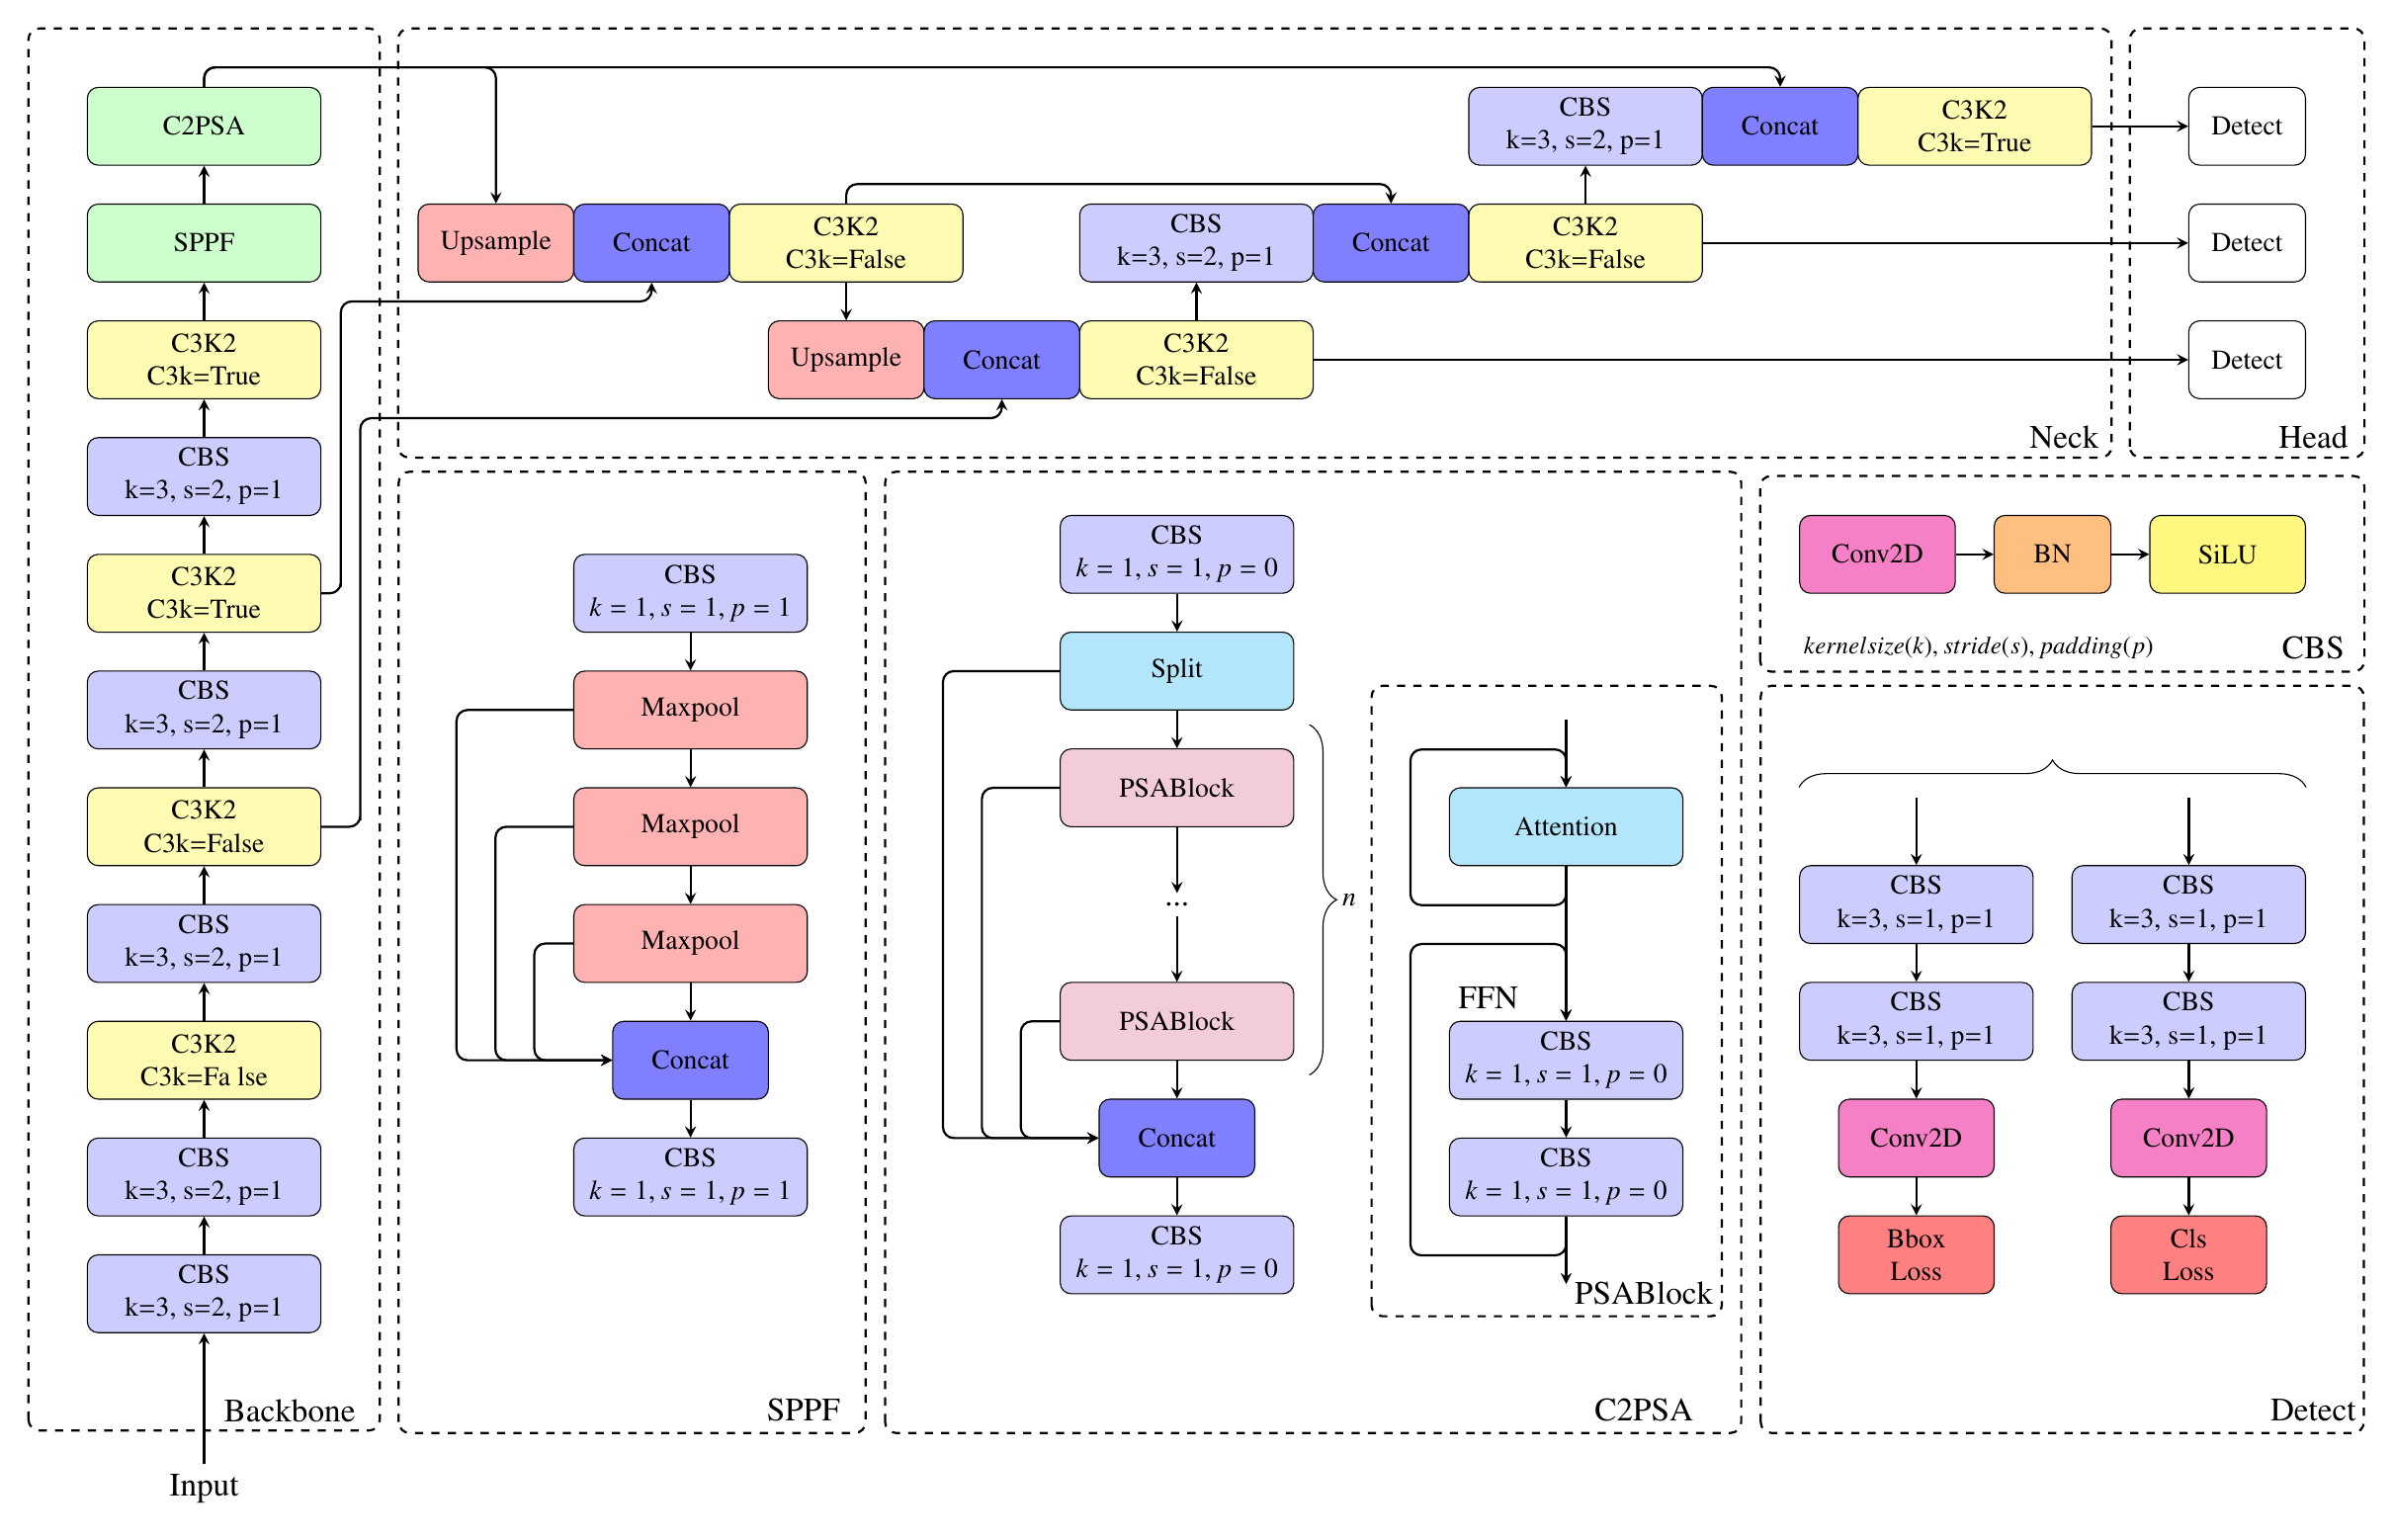
\begin{tikzpicture}[node distance=1.5cm]
% Backbone Nodes
\node (input) [label] {Input};
\node (cbs0) [cbs, above of=input, yshift=1cm] {CBS\\k=3, s=2, p=1};
\node (cbs1) [cbs, above of=cbs0] {CBS\\k=3, s=2, p=1};
\node (c3k2_1) [c3k2, above of=cbs1] {C3K2\\C3k=Fa  lse};
\node (cbs2) [cbs, above of=c3k2_1] {CBS\\k=3, s=2, p=1};
\node (c3k2_2) [c3k2, above of=cbs2] {C3K2\\C3k=False};
\node (cbs3) [cbs, above of=c3k2_2] {CBS\\k=3, s=2, p=1};
\node (c3k2_3) [c3k2, above of=cbs3] {C3K2\\C3k=True};
\node (cbs4) [cbs, above of=c3k2_3] {CBS\\k=3, s=2, p=1};
\node (c3k2_4) [c3k2, above of=cbs4] {C3K2\\C3k=True};
\node (sppf) [layer, above of=c3k2_4, fill=green!20, align=center] {SPPF};
\node (c2psa) [layer, above of=sppf, fill=green!20, align=center] {C2PSA};

% Neck Nodes
\node (up1) [upsample, right of=sppf, xshift=2.25cm, minimum width=2cm] {Upsample};
\node (cc1) [concat, right of=up1, xshift=.5cm] {Concat};
\node (c3k2_5) [c3k2, right of=cc1, xshift=1cm] {C3K2\\C3k=False};

\node (up2) [upsample, below of=c3k2_5, minimum width=2cm] {Upsample};
\node (cc2) [concat, right of=up2, xshift=.5cm] {Concat};
\node (c3k2_6) [c3k2, right of=cc2, xshift=1cm] {C3K2\\C3k=False};

\node (cbs5) [cbs, above of=c3k2_6] {CBS\\k=3, s=2, p=1};
\node (cc3) [concat, right of=cbs5, xshift=1cm] {Concat};
\node (c3k2_7) [c3k2, right of=cc3, xshift=1cm] {C3K2\\C3k=False};

\node (cbs6) [cbs, above of=c3k2_7] {CBS\\k=3, s=2, p=1};
\node (cc4) [concat, right of=cbs6, xshift=1cm] {Concat};
\node (c3k2_8) [c3k2, right of=cc4, xshift=1cm] {C3K2\\C3k=True};

% Head Nodes
\node (detect1) [detect,  right of=c3k2_8, xshift=2cm] {Detect};
\node (detect2) [detect, below of=detect1] {Detect};
\node (detect3) [detect, below of=detect2] {Detect};

% SPPF Diagram
\node (cbs7) [cbs, right of=c3k2_3, xshift=4.75cm] {CBS \\ $k=1, s=1, p=1$};
\node (maxpool1) [layer, fill=red!30, below of=cbs7] {Maxpool};
\node (maxpool2) [layer, fill=red!30, below of=maxpool1] {Maxpool};
\node (maxpool3) [layer, fill=red!30, below of=maxpool2] {Maxpool};
\node (cc5) [concat, fill=blue!50, below of=maxpool3] {Concat};
\node (cbs8) [cbs, below of=cc5] {CBS \\ $k=1, s=1, p=1$};

% C2PSA Diagram
\node (cbs9) [cbs, right of=cbs7, xshift=4.75cm, yshift=.5cm] {CBS \\ $k=1, s=1, p=0$};
\node (split1) [layer, fill=cyan!30, below of=cbs9] {Split};
\node (PSA1) [layer, fill=purple!20, below of=split1] {PSABlock};
\node (dots) [label, below of=PSA1] {...};
\node (PSA2) [layer, fill=purple!20, below of=dots] {PSABlock};
\node (cc6) [concat, fill=blue!50, below of=PSA2] {Concat};
\node (cbs10) [cbs, below of=cc6] {CBS \\ $k=1, s=1, p=0$};

\node (attention) [layer, fill=cyan!30, right of=maxpool2, xshift=9.75cm] {Attention};
\node (cbs11) [cbs, below of=attention, yshift=-1.5cm] {CBS \\ $k=1, s=1, p=0$};
\node (cbs12) [cbs, below of=cbs11] {CBS \\ $k=1, s=1, p=0$};
\node (n1) [label, below of=cbs12] { };
\node (ffn) [label, above of=cbs11, xshift=-1cm, yshift=-.7cm] {FFN};
\node (h1) [label, above of=attention] { };

% CBS
\node (conv2d) [conv2D, right of=cbs9, minimum width=2cm, xshift=7.5cm] {Conv2D};
\node (bN) [layer, right of=conv2d, fill=orange!50, minimum width=1.5cm, xshift=.75cm] {BN};
\node (siLU) [layer, right of=bN, fill=yellow!50, minimum width=2cm, xshift=.75cm] {SiLU};

% Detection
\node (cbs22) [cbs, right of=PSA2, xshift=8cm] {CBS\\k=3, s=1, p=1};
\node (cbs21) [cbs, above of=cbs22] {CBS\\k=3, s=1, p=1};
\node (conv2d_1) [conv2D, below of=cbs22] {Conv2D};
\node (bbox) [layer, below of=conv2d_1, fill=red!50, minimum width=2cm,] {Bbox\\Loss};
\node (h2) [label, above of=cbs21] { };

\node (cbs31) [cbs, right of=cbs21, xshift=2cm] {CBS\\k=3, s=1, p=1};
\node (cbs32) [cbs, below of=cbs31] {CBS\\k=3, s=1, p=1};
\node (conv2d_2) [conv2D, below of=cbs32] {Conv2D};
\node (cls) [layer, below of=conv2d_2, fill=red!50, minimum width=2cm,] {Cls\\Loss};
\node (h3) [label, above of=cbs31] { };

% Labels
\node (Bone) [label, below of=cbs0, xshift=1.1cm] {Backbone};
\node (SPPF) [label, right of=Bone, xshift=5.1cm] {SPPF};
\node (C2PSA)[label, right of=SPPF, xshift=9.3cm] {C2PSA};
\node (PSABlock) [label, above of=C2PSA] {PSABlock};
\node (Detect) [label, right of=C2PSA, xshift=7.1cm] {Detect};
\node (CBS) [label, above of=Detect, yshift=8.3cm] {CBS};
\node (legend) [label, font=\small, left of=CBS, xshift=-2.8cm] {$kernel size(k), stride(s), padding(p)$};
\node (Head) [label, above of=CBS, yshift=1.2cm] {Head};
\node (Neck) [label, left of=Head, xshift=-1.7cm] {Neck};

% Blocks
\draw [dashed, thick, rounded corners] ($(cbs0.south west) - (.75,1.25)$) rectangle ($(c2psa.north east) + (.75,.75)$);
\draw [dashed, thick, rounded corners] ($(up1.south west) - (.25,2.25)$) rectangle ($(c3k2_8.north east) + (.25,.75)$);
\draw [dashed, thick, rounded corners] ($(detect3.south west) - (.75,.75)$) rectangle ($(detect1.north east) + (.75,.75)$);
\draw [dashed, thick, rounded corners] ($(conv2d.south west) - (.5,1)$) rectangle ($(siLU.north east) + (.75,.5)$);
\draw [dashed, thick, rounded corners] (2.5,.4) rectangle (8.5,12.75);
\draw [dashed, thick, rounded corners] (8.75,.4) rectangle (19.75,12.75);
\draw [dashed, thick, rounded corners] (15,1.9) rectangle (19.5,10);
\draw [dashed, thick, rounded corners] (20,.4) rectangle (27.75,10);

% Bracket for repeated layers
\draw [decorate, decoration={brace, amplitude=10pt}] 
    (14.2,9.5) -- (14.2,5) 
    node[midway, right=.3] {$n$};
\draw [decorate, decoration={brace, amplitude=10pt}] 
    ($(cbs21.north west)+(0,1)$) -- ($(cbs31.north east)+(0,1)$)
    node[midway, right=.3] { };

\draw [arrow] (maxpool1.west) -| +(-1.5,-1) |- (cc5);
\draw [arrow] (maxpool2.west) -| +(-1,-1) |- (cc5);
\draw [arrow] (maxpool3.west) -| +(-.5,-1) |- (cc5);
\draw [arrow] (split1.west) -| +(-1.5,-1) |- (cc6);
\draw [arrow] (PSA1.west) -| +(-1,-1) |- (cc6);
\draw [arrow] (PSA2.west) -| +(-.5,-1) |- (cc6);
\draw [arrow] (attention.south) |- +(0,-.5) -| ++(-2,0) |- ++(1,1.5) -| (attention.north);
\draw [arrow] (cbs12.south) |- +(0,-.5) -| ++(-2,0) |- ++(1,3.5) -| (cbs11.north);


% Arrows Backbone
\draw [arrow] (input) -- (cbs0);
\draw [arrow] (cbs0) -- (cbs1); 
\draw [arrow] (cbs1) -- (c3k2_1);
\draw [arrow] (c3k2_1) -- (cbs2);
\draw [arrow] (cbs2) -- (c3k2_2);
\draw [arrow] (c3k2_2) -- (cbs3);
\draw [arrow] (cbs3) -- (c3k2_3);
\draw [arrow] (c3k2_3) -- (cbs4);
\draw [arrow] (cbs4) -- (c3k2_4);
\draw [arrow] (c3k2_4) -- (sppf);
\draw [arrow] (sppf) -- (c2psa);

% Arrows Neck
\draw [arrow] (c3k2_3.east) -| +(.25,0) |- +(1,3.75) -| (cc1);
\draw [arrow] (c3k2_2.east) -| +(.5,0) |- +(1,5.25) -| (cc2);
\draw [arrow] (c3k2_5.north) |- +(1,.25) -| (cc3);
\draw [arrow] (c2psa.north) |- +(1,.25) -| (cc4);
\draw [arrow] (c2psa.north) |- +(1,.25) -| (up1);
\draw [arrow] (c3k2_5) -- (up2);
\draw [arrow] (c3k2_6) -- (cbs5);
\draw [arrow] (c3k2_7) -- (cbs6);

% Arrow Head
\draw [arrow] (c3k2_8) -- (detect1);
\draw [arrow] (c3k2_7) -- (detect2);
\draw [arrow] (c3k2_6) -- (detect3);

\draw [arrow] (cbs7) -- (maxpool1);
\draw [arrow] (maxpool1) -- (maxpool2);
\draw [arrow] (maxpool2) -- (maxpool3);
\draw [arrow] (maxpool3) -- (cc5);
\draw [arrow] (cc5) -- (cbs8);

\draw [arrow] (cbs9) -- (split1);
\draw [arrow] (split1) -- (PSA1);
\draw [arrow] (PSA1) -- (dots);
\draw [arrow] (dots) -- (PSA2);
\draw[arrow] (PSA2) -- (cc6);
\draw[arrow] (cc6) -- (cbs10);

\draw[arrow] (h1) -- (attention);
\draw[arrow] (attention) -- (cbs11);
\draw[arrow] (cbs11) -- (cbs12);
\draw[arrow] (cbs12) -- (n1);

\draw[arrow] (conv2d) -- (bN);
\draw[arrow] (bN) -- (siLU);

\draw[arrow] (h2) -- (cbs21);
\draw[arrow] (cbs21) -- (cbs22);
\draw[arrow] (cbs22) -- (conv2d_1);
\draw[arrow] (conv2d_1) -- (bbox);

\draw[arrow] (h3) -- (cbs31);
\draw[arrow] (cbs31) -- (cbs32);
\draw[arrow] (cbs32) -- (conv2d_2);
\draw[arrow] (conv2d_2) -- (cls);
\end{tikzpicture}
  }
  \caption{Arsitektur Yolov11}
  \label{fig:ArsitekturYolov11}
\end{figure}

Arsitektur \emph{C3K2} merupakan versi yang dimodifikasi dari modul \emph{C2F}. Perbedaan utama terletak pada konfigurasi parameter \emph{c3k}. Ketika \emph{c3k} disetel ke \texttt{False}, modul \emph{C3K2} berperilaku seperti modul \emph{C2F}, menggunakan struktur \emph{bottleneck} standar. Sebaliknya, ketika \emph{c3k} disetel ke \texttt{True}, modul \emph{bottleneck} digantikan oleh modul \emph{C3}. Perubahan ini dapat dilihat pada gambar berikut.

\begin{figure}[H]
  \centering
  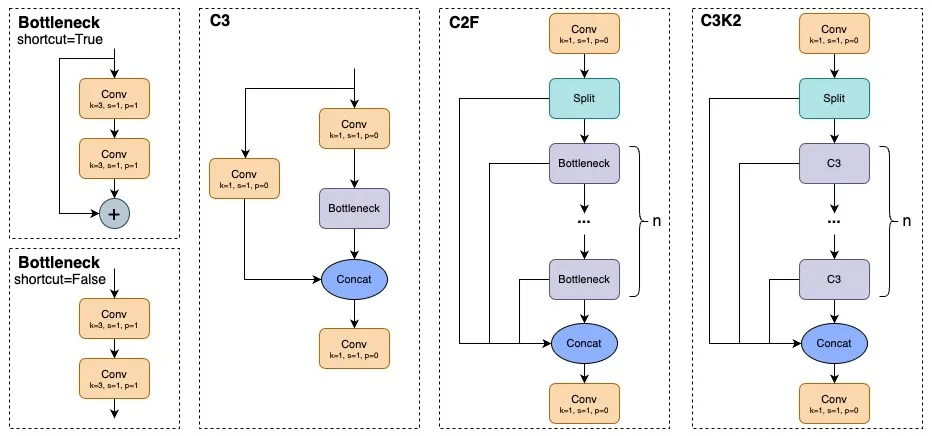
\includegraphics[scale=0.55]{gambar/C3k2.jpg}
  \caption{Modul Bottleneck, C3, C2F, dan C3K2}
  \label{fig:c3k2}
\end{figure}

Fitur input diubah pada lapisan \emph{feedforward} ke dalam ruang berdimensi lebih tinggi, sehingga hubungan non-linear yang kompleks dapat tertangkap dengan lebih stabil.

\section{MediaPipe}
\label{sec:MediaPipe}

\emph{MediaPipe} adalah framework \emph{open-source} yang dikembangkan oleh Google untuk membangun pipeline pemrosesan media yang efisien, termasuk dalam pengolahan gambar dan video. Framework ini menyediakan berbagai modul yang dapat dimanfaatkan untuk aplikasi seperti deteksi wajah, pelacakan tangan, dan estimasi pose.

Kerangka kerja \emph{MediaPipe} menggunakan konsep "graph," di mana setiap node dalam graph berfungsi sebagai "calculator" yang menjalankan tugas spesifik, seperti deteksi objek, pelacakan pose, atau segmentasi gambar. Konfigurasi node-node ini dapat disesuaikan melalui \emph{GraphConfig}, yang mendefinisikan topologi dan fungsionalitas dari keseluruhan sistem.

\begin{figure}[H]
  \centering
  \includegraphics[scale=0.5]{gambar/MediaPipe3D.png}
  \caption{MediaPipe 3D.}
  \label{fig:MediaPipe3D}
\end{figure}

Salah satu contoh penggunaan \emph{MediaPipe} yang paling dikenal adalah estimasi pose manusia menggunakan modul \emph{MediaPipe Pose}. Teknik ini mengombinasikan estimasi pose 2D dengan model humanoid yang lebih kompleks, serta menggunakan metode optimasi untuk menghitung sudut sendi dalam pose 3D. Pendekatan ini efektif dalam mengatasi masalah ambiguitas kedalaman pada estimasi pose 3D, dan mampu bekerja secara \emph{real-time}. Visualisasi pose 3D yang dihasilkan memperlihatkan setiap sendi tubuh sebagai titik dan garis penghubung antar sendi, memberikan gambaran yang jelas mengenai posisi dan orientasi tubuh di dalam ruang 3D.

\subsection{MediaPipe Pose}
\label{subsec:MediaPipe Pose}

\emph{MediaPipe Pose} adalah modul dalam \emph{MediaPipe} yang dirancang khusus untuk mendeteksi dan melacak pose manusia secara \emph{real-time}. Dengan menggunakan model \emph{machine learning} yang canggih, \emph{MediaPipe Pose} dapat mengidentifikasi hingga 33 titik referensi pada tubuh manusia, memungkinkan sistem untuk memahami dan merespons gerakan pengguna secara cepat dan akurat.

\begin{figure}[H]
  \centering
  \includegraphics[scale=0.5]{gambar/mp_pose.jpg}
  \caption{MediaPipe Pose.}
  \label{fig:mp_pose}
\end{figure}

\section{Classification Performance}
\label{sec:Classification Performance}

\emph{Classification performance} mengacu pada kemampuan model untuk mengklasifikasikan data input ke dalam kategori yang benar. Proses pengklasifikasian memerlukan evaluasi untuk menilai efektivitas model yang telah dikembangkan, biasanya dengan menggunakan set data pengetesan. Salah satu pendekatan evaluasi yang sering digunakan dalam konteks pengklasifikasian adalah \emph{confusion matrix}, yang memberikan visualisasi mengenai kinerja model dalam mengategorikan data secara akurat.

\begin{figure}[H]
  \centering
  \includegraphics[scale=0.5]{gambar/Matrix Konfusi.jpg}
  \caption{Matrix Konfusi.}
  \label{fig:confusion}
\end{figure}

\emph{Confusion matrix} ini digunakan untuk mengevaluasi kinerja model klasifikasi biner dan menampilkan empat jenis hasil dari prediksi model: \emph{True Positive} (TP), \emph{False Negative} (FN), \emph{False Positive} (FP), dan \emph{True Negative} (TN). TP terjadi ketika model memprediksi kelas positif dengan benar, sedangkan FN terjadi ketika model salah memprediksi kelas negatif padahal seharusnya positif (disebut juga sebagai \emph{Type II Error}). FP terjadi ketika model salah memprediksi kelas positif padahal seharusnya negatif (disebut juga sebagai \emph{Type I Error}), dan TN terjadi ketika model memprediksi kelas negatif dengan benar.

\section{Evaluation Metrics}
\label{sec:Evaluation Metrics}

Metrik evaluasi berfungsi sebagai dasar pemahaman dalam membandingkan efektivitas berbagai algoritma dan skenario yang berbeda. Melalui evaluasi yang teliti, perbandingan akurat antara berbagai teknik deteksi objek dapat dilakukan, serta tingkat keakuratan yang dicapai dapat dinilai dengan tepat. Hal ini menjadi sangat penting dalam pemilihan algoritma yang paling sesuai untuk tugas deteksi tertentu. Metrik seperti \emph{akurasi}, \emph{presisi}, dan \emph{recall} digunakan untuk mengevaluasi efektivitas model dalam mendeteksi dan mengidentifikasi objek dengan benar. Implementasi metrik-metrik ini diperlukan untuk menentukan model yang paling efisien.

Selain itu, analisis akurasi memberikan wawasan kuantitatif yang signifikan mengenai kinerja algoritma deteksi objek, serta detail lebih lanjut mengenai kemampuan algoritma dalam menghasilkan deteksi yang akurat. Kesalahan yang teridentifikasi melalui metrik evaluasi menjadi langkah penting dalam penelitian deteksi, seperti dalam kasus deteksi asap yang diteliti. Identifikasi ini memudahkan pemahaman mengenai potensi kesalahan dalam algoritma, yang kemudian dapat mengarah pada perbaikan dan peningkatan metode deteksi. Metrik evaluasi juga dimanfaatkan untuk mendukung pengoptimalan hiperparameter algoritma.

Dalam penelitian ini, berbagai metrik evaluasi seperti \emph{presisi}, \emph{recall}, dan \emph{Mean Average Precision} (mAP) telah diterapkan. Dengan menggabungkan metode evaluasi ini, penelitian ini dirancang untuk menyajikan analisis komprehensif mengenai kinerja algoritma deteksi objek yang ditinjau. Penjelasan mengenai konsep dasar metrik evaluasi akan dijabarkan sebagai berikut:

\subsection{Precision}
\label{subsec:precision}

\emph{Precision} merupakan salah satu metrik utama yang digunakan untuk mengukur seberapa akurat prediksi dari model terhadap objek yang terdeteksi. Metrik ini menunjukkan proporsi prediksi positif yang benar (\emph{True Positive}) dibandingkan dengan keseluruhan prediksi positif, baik yang benar (\emph{True Positive}) maupun salah (\emph{False Positive}), yang dinyatakan dengan persamaan berikut: 
\begin{equation} 
  \mathrm{Precision} = \frac{TP}{TP + FP} 
\end{equation}

Di mana \(TP\) (\emph{True Positive}): Prediksi benar, yaitu deteksi objek yang sesuai dengan \emph{ground truth} dan \(FP\) (\emph{False Positive}): Prediksi salah, yaitu deteksi objek yang tidak sesuai dengan \emph{ground truth}.

\emph{Precision} sangat berguna dalam situasi di mana kesalahan prediksi positif (\emph{false positive}) harus diminimalkan. Contohnya, dalam aplikasi kursi roda otonom, deteksi yang salah terhadap manusia dapat menyebabkan tindakan yang berbahaya, sehingga \emph{precision} harus dipertahankan pada nilai yang tinggi.

\emph{Precision} biasanya dikombinasikan dengan metrik lain, seperti \emph{recall}, untuk memberikan gambaran yang lebih lengkap tentang kinerja model.

\subsection{Recall}
\label{subsec:recall}

\emph{Recall} atau sensitivitas mengukur kemampuan model dalam mendeteksi semua objek yang ada pada gambar atau video. \emph{Recall} menekankan pada seberapa banyak objek yang benar-benar ada dalam data (\emph{ground truth}) yang berhasil terdeteksi oleh model dengan persamaan berikut:

\begin{equation} 
  \mathrm{Recall} = \frac{TP}{TP + FN} 
\end{equation}

Di mana \(TP\) (\emph{True Positive}): Prediksi benar, yaitu objek yang terdeteksi dengan benar dan \(FP\) (\emph{False Negative}): Prediksi salah, yaitu objek yang ada tetapi tidak terdeteksi.

Metrik ini penting ketika kesalahan berupa kegagalan dalam mendeteksi objek (\emph{false negative}) harus diminimalkan. Dalam konteks pengembangan kursi roda otonom, \emph{recall} sangat penting karena objek seperti manusia harus selalu terdeteksi agar kursi roda dapat mengikuti secara akurat.

\textbf{\emph{Trade-off Precision dan Recall:}} Dalam banyak kasus, \emph{precision} dan \emph{recall} memiliki hubungan yang berlawanan. Jika model terlalu konservatif dalam membuat prediksi, \emph{precision} akan tinggi, tetapi \emph{recall} rendah. Sebaliknya, jika model terlalu longgar dalam mendeteksi objek, \emph{recall} tinggi tetapi \emph{precision} menurun. Oleh karena itu, diperlukan keseimbangan antara \emph{precision} dan \emph{recall}, yang biasanya diekspresikan melalui metrik lain seperti \emph{F1-score}.

\subsection{Mean Average Precision (mAP)}
\label{subsec:mAP}

\emph{Mean Average Precision} (mAP) merupakan metrik komprehensif yang digunakan untuk mengukur performa model deteksi objek secara keseluruhan. \emph{mAP} adalah rata-rata dari \emph{average precision} (AP) di berbagai kelas yang ada dalam dataset.

\begin{equation} 
  \mathrm{AP} = \int_0^1 P(r) , dr 
\end{equation}

Di mana \(P(r)\) : \emph{Precision} sebagai fungsi dari \emph{recall} dan \(dr\) : Diferensial dari \emph{recall}.

AP dihitung dengan mencari area di bawah kurva \emph{precision-recall} (\emph{PR curve}) untuk setiap kelas. Setelah AP untuk semua kelas dihitung, rata-rata dari nilai-nilai tersebut akan memberikan nilai \emph{mAP}.

\begin{equation} 
  \mathrm{mAP} = \frac{1}{N} \sum_{i=1}^{N} \mathrm{AP}_i 
\end{equation}

Di mana \(N\) : Jumlah kelas dalam dataset dan \(AP_i\) : \emph{Average precision} untuk kelas ke-i.

\emph{mAP} memberikan gambaran yang lebih luas mengenai performa detektor objek, karena metrik ini mempertimbangkan baik \emph{precision} maupun \emph{recall} secara bersamaan. Nilai \emph{mAP} ini akan menjadi acuan untuk mengevaluasi performa sistem, seperti mendeteksi berbagai objek seperti manusia, rintangan, dan lingkungan sekitar.

\subsection{Intersection over Union (IoU)}
\label{subsec:IoU}

\emph{Intersection over Union} (\emph{IoU}) adalah metrik yang digunakan untuk mengevaluasi keakuratan deteksi posisi objek yang dilakukan oleh model dalam pemrosesan gambar. Area persinggungan antara kotak deteksi yang dihasilkan oleh model dan kotak referensi, yang dikenal sebagai \emph{Ground Truth}, dihitung untuk menilai kinerja model. Rasio ini diperoleh dengan membandingkan luas area irisan dari kedua kotak tersebut terhadap total luas area gabungan yang mereka cakup. Jika kedua kotak tersebut diperlakukan sebagai satu kesatuan, maka \emph{IoU} memberikan skor yang menunjukkan seberapa akurat model dalam memprediksi lokasi objek yang sebenarnya. Nilai \emph{IoU} akan semakin tinggi seiring dengan bertambahnya proporsi area persinggungan relatif terhadap keseluruhan area gabungan.

\begin{figure}[H]
  \centering
  \includegraphics[scale=0.27]{gambar/IoU bbox.jpg}
  \caption{Intersection over Union.}
  \label{fig:IoU bbox}
\end{figure}

Kinerja model deteksi objek dilakukan evaluasi kinerja model deteksi objek dengan cara membandingkan area tumpang tindih antara \emph{bounding box} prediksi dan \emph{bounding box} \emph{ground truth}. Nilai \emph{IoU} berkisar antara 0 hingga 1, di mana nilai yang lebih mendekati 1 menunjukkan tingkat akurasi yang lebih tinggi dalam deteksi dan penentuan lokasi objek.

Dalam proses evaluasi, \emph{bounding box} yang dihasilkan oleh model dibandingkan dengan \emph{bounding box ground truth}, yang ditentukan secara manual sebagai lokasi sebenarnya dari objek dalam citra. Perhitungan \emph{IoU} dilakukan dengan membagi luas area tumpang tindih antara kedua \emph{bounding box} tersebut dengan luas total area gabungan dari keduanya. Persamaan berikut digunakan untuk menghitung nilai \emph{IoU}: 

\begin{equation}
  IoU = \frac{\left |A\bigcap B  \right |}{\left | A\bigcup B \right |}.
\end{equation}

\emph{IoU} dipilih sebagai alat ukur karena kemampuannya untuk memberikan penilaian yang jelas tentang seberapa akurat model dalam mengidentifikasi dan membatasi objek di berbagai kondisi, termasuk variasi ukuran, orientasi, dan konteks objek dalam citra. Nilai \emph{IoU} yang lebih tinggi diindikasikan sebagai tanda bahwa model dapat diandalkan dalam mendeteksi dan mengidentifikasi objek dengan tingkat presisi yang tinggi.

\section{Tinjauan Pustaka BoT-SORT}

BoT-SORT merupakan salah satu metode multi-object tracking (MOT) yang dikembangkan dengan pendekatan tracking-by-detection. Pada prinsipnya, metode ini memanfaatkan beberapa teknik dari berbagai algoritma sebelumnya, terutama ByteTrack, untuk menyajikan pelacakan yang lebih canggih. Perbaikan pada metode ini bertujuan untuk meningkatkan kinerja pelacakan dalam lingkungan dinamis maupun statis dengan memperbaiki beberapa komponen utama, yang akan dijabarkan sebagai berikut \parencite{aharon2022botsortrobustassociationsmultipedestrian}:

\subsection{Kalman Filter}

Kalman Filter (KF) berfungsi untuk memprediksi lokasi objek di frame berikutnya berdasarkan pergerakan sebelumnya. BoT-SORT menggunakan KF dengan vektor status yang mencakup koordinat pusat objek ($x_c$, $y_c$), lebar ($w$), tinggi ($h$), dan laju perubahan (kecepatan) dari variabel-variabel tersebut ($\dot{x_c}$, $\dot{y_c}$, $\dot{w}$, $\dot{h}$) \parencite{bewley2016simple, wojke2017simple}. Vektor status ini didefinisikan sebagai:

\begin{equation}
  \begin{split}
    \vb*{x}_k = [x_{c}{\scriptstyle(k)}, y_{c}{\scriptstyle(k)}, w{\scriptstyle(k)}, h{\scriptstyle(k)}, \\        
    \dot{x_{c}}{\scriptstyle(k)}, \dot{y_{c}}{\scriptstyle(k)}, \dot{w}{\scriptstyle(k)}, \dot{h}{\scriptstyle(k)}]^\top
  \end{split}
\end{equation}

\begin{equation}
  \vb*{z}_k = [z_{x_c}{\scriptstyle(k)}, z_{y_c}{\scriptstyle(k)}, z_{w}{\scriptstyle(k)}, z_{h}{\scriptstyle(k)}]^\top
\end{equation}

Matriks noise proses ($\mathbf{Q}_k$) dan noise pengukuran ($\mathbf{R}_k$) disesuaikan agar lebih sensitif terhadap perubahan dalam frame, yang membantu meningkatkan akurasi pelacakan. Matriks $\mathbf{Q}_k$ dan $\mathbf{R}_k$ ditentukan sebagai berikut:

\begin{equation}
  \begin{split}
    \vb*{Q}_k = diag\big{(} (\sigma_{p} \hat{w}_{k-1|k-1})^2, (\sigma_{p} \hat{h}_{k-1|k-1})^2, \\
    (\sigma_{p} \hat{w}_{k-1|k-1})^2, (\sigma_{p} \hat{h}_{k-1|k-1})^2, \\
    (\sigma_{v} \hat{w}_{k-1|k-1})^2, (\sigma_{v} \hat{h}_{k-1|k-1})^2, \\ 
    (\sigma_{v} \hat{w}_{k-1|k-1})^2 ,(\sigma_{v} \hat{h}_{k-1|k-1})^2\big{)}
  \end{split}
\end{equation}

\begin{equation}
  \begin{split}
      \vb*{R}_k = diag\big{(}(\sigma_{m} \hat{w}_{k|k-1})^2, (\sigma_{m} \hat{h}_{k|k-1})^2, \\
      (\sigma_{m} \hat{w}_{k|k-1})^2, (\sigma_{m} \hat{h}_{k|k-1})^2\big{)} 
  \end{split}
\end{equation}

Dengan adanya perubahan ini, prediksi \emph{bounding box} lebih akurat dibandingkan dengan metode Kalman Filter tradisional, terbukti dengan peningkatan nilai HOTA (Higher Order Tracking Accuracy).

\begin{figure}[H]
  \centering
  \includegraphics[scale=0.3]{gambar/KF_width.png}
  \caption{Kalman Filter bbox.}
  \label{fig:KF width}
\end{figure}

Visualisasi bentuk \emph{bounding box} dibandingkan dengan \emph{Kalman filter} yang banyak digunakan~\parencite{wojke2017simple} (biru putus-putus) dan \emph{Kalman filter} yang diusulkan (hijau). Tampak bahwa lebar \emph{bounding box} yang dihasilkan oleh \emph{Kalman filter} yang diusulkan lebih sesuai dengan objek. \emph{Bounding box} biru putus-putus memotong bagian kaki objek (dalam merah), sedangkan \emph{bounding box} hijau mencapai lebar yang diinginkan.

\subsection{\emph{Camera Motion Compensation} (CMC)}

Pelacak berbasis tracking-by-detection seringkali mengalami masalah ID switch atau false negatives akibat gerakan kamera, terutama dalam situasi dinamis. BoT-SORT mengimplementasikan teknik kompensasi gerakan kamera (Camera Motion Compensation) dengan memanfaatkan affine transformation untuk menghitung transformasi antara dua frame. Dengan melakukan ekstraksi keypoints gambar ~\cite{shi1994good}, kemudian menggunakan sparse optical flow ~\cite{Bouguet1999PyramidalIO} untuk pelacakan fitur dengan penolakan outlier lokal berbasis translasi. Matriks affine $\vb*{A}_{k-1}^k\in \mathbb{R}^{2 \times 3}$ diselesaikan menggunakan metode RANSAC ~\cite{fischler1981random}. Penggunaan teknik pendaftaran spars memungkinkan pengabaian objek dinamis dalam adegan berdasarkan deteksi, sehingga memiliki potensi untuk memperkirakan gerakan latar belakang dengan lebih akurat.

\begin{equation}
  \begin{aligned}
      & \vb*{A}_{k-1}^k = 
      \begin{bmatrix}
          \vb*{M}_{2x2} | \vb*{T}_{2x1}
      \end{bmatrix} = 
      \begin{bmatrix}
          a_{11}\;a_{12}\;a_{13} \\ a_{21}\;a_{22}\;a_{23} \\ 
      \end{bmatrix}
  \end{aligned}
\end{equation}
\begin{equation}
  \begin{aligned}
  {
      \vb*{\tilde{M}}}^k_{k-1} = 
      \begin{bmatrix}
      \vb*{M} & \vb*{0} & \vb*{0} & \vb*{0} \\
      \vb*{0} & \vb*{M} & \vb*{0} & \vb*{0} \\
      \vb*{0} & \vb*{0} & \vb*{M} & \vb*{0} \\
      \vb*{0} & \vb*{0} & \vb*{0} & \vb*{M}
      \end{bmatrix}, \; 
      \tilde{\vb*{T}}_{k-1}^k = 
      \begin{bmatrix}a_{13}\\a_{23}\\ 0\\ 0\\ \vdots \\ 0\end{bmatrix}
  \end{aligned}
\end{equation}
\begin{equation}
  \begin{aligned}
      \hat{\vb*{x}}^\prime_{k|k-1} = \tilde{\vb*{M}}_{k-1}^k \hat{\vb*{x}}_{k|k-1} + \tilde{\vb*{T}}_{k-1}^k \\
  \end{aligned}
\end{equation}
\begin{equation}
    {{\vb*{P}}}^{\prime}_{k|k-1} = 
    \tilde{\vb*{M}}_{k-1}^k {\vb*{P}}_{k|k-1} {\tilde{\vb*{M}}_{k-1}}^{k^\top}
    \label{eq:cmc_cov}        
\end{equation}

Dimana $\vb*{M}\in \mathbb{R}^{2 \times 2}$ merupakan matriks yang berisi skala dan rotasi dari matriks afine $\vb*{A}$, dan $T$ mengandung komponen translasi. Trik matematis digunakan dengan mendefinisikan $\tilde{\vb*{M}}^k_{k-1}\in \mathbb{R}^{8 \times 8}$ dan $\tilde{\vb*{T}}_{k-1}^k\in \mathbb{R}^{8}$. Selanjutnya, $\hat{\vb*{x}}_{k|k-1}$ dan $\hat{\vb*{x}}^\prime_{k|k-1}$ didefinisikan sebagai vektor status prediksi dari Kalman Filter (KF) pada waktu $k$, sebelum dan setelah kompensasi gerakan kamera, sedangkan $\vb*{P}_{k|k-1}$ dan $\vb*{P'}_{k|k-1}$ didefinisikan sebagai matriks kovarians KF sebelum dan setelah koreksi. Setelah itu, $\hat{\vb*{x}}^\prime_{k|k-1}$ dan ${{\hat{\vb*{P}}}^{\prime}}_{k|k-1}$ digunakan dalam langkah update Kalman Filter sebagai berikut.

\begin{equation}
  \begin{aligned}
  & \vb*{K_k} =  {{\vb*{P}}}^{\prime}_{k|k-1} \vb*{H}_k^\top (\vb*{H}_k  {{\vb*{P}}}^{\prime}_{k|k-1} \vb*{H}_k^\top + \vb*{R}_k)^{-1} \\
  & \hat{\vb*{x}}_{k|k} = \hat{\vb*{x}}^\prime_{k|k-1} + \vb*{K}_k (\vb*{z}_k - \vb*{H}_k \hat{\vb*{x}}^\prime_{k|k-1}) \\
  & \vb*{P}_{k|k} = (\vb*{I}- \vb*{K}_k \vb*{H}_k)  {{\vb*{P}}}^{\prime}_{k|k-1}
  \end{aligned}
  \label{eq:cmc_update_kf}
\end{equation} 
`'
Dalam skenario kecepatan tinggi, koreksi penuh terhadap vektor status, termasuk komponen kecepatan, sangat penting. Jika kamera berubah dengan lambat dibandingkan dengan kecepatan frame, koreksi pada persamaan \ref{eq:cmc_cov} dapat diabaikan. Setelah mengompensasi gerakan kamera yang rigid dan dengan asumsi posisi objek hanya sedikit berubah dari satu frame ke frame berikutnya, pada aplikasi dengan frame rate tinggi, ketika deteksi hilang, prediksi lintasan dapat dilakukan menggunakan langkah prediksi KF, yang memungkinkan tampilan lintasan yang lebih kontinu dan MOTA yang lebih tinggi.

Visualisasi prediksi \emph{bounding box} (BB) dari tracklet digunakan untuk asosiasi dengan BB deteksi baru berdasarkan kriteria IoU maksimum. (a.1) dan (b.1) memperlihatkan prediksi dari Kalman Filter (KF). (a.2) dan (b.2) memperlihatkan prediksi dari KF setelah kompensasi gerakan kamera. Pada gambar (b.1), diperlihatkan skenario di mana pengabaian gerakan kamera dapat menyebabkan IDSWs atau FN. Sebaliknya, pada gambar (b.2), prediksi telah sesuai dengan lokasi yang diinginkan dan asosiasi berhasil dilakukan. Gambar \ref{fig:cmc} dihasilkan dari sekuens MOT17 \cite{milan2016mot16}, yang mencakup pergerakan kamera akibat manuver kendaraan yang berbelok ke arah kanan.

\begin{figure}[H]
  \centering
  \includegraphics[scale=0.35]{gambar/cmc_pred.png}
  \label{fig:cmc}
  \caption{Kompensasi Gerakan Kamera}
\end{figure}

\subsection{Fusi IoU - Re-ID}

Fitur Re-ID diintegrasikan untuk memanfaatkan kemajuan dalam representasi visual objek. Fitur Re-ID diekstraksi menggunakan FastReID dengan backbone ResNeSt50 \parencite{he2020fastreid, zhang2020resnest}, dan mekanisme exponential moving average (EMA) digunakan untuk memperbarui status appearance tracklet \parencite{wang2020towards}. Pembaruan status appearance dilakukan dengan rumus:

\begin{equation}
e_i^k = \alpha e_i^{k-1} + (1 - \alpha) f_i^k
\end{equation}

Di mana $e_i^k$ adalah status appearance untuk tracklet ke-$i$ pada frame $k$, $f_i^k$ adalah embedding appearance deteksi saat ini, dan $\alpha=0.9$ adalah momentum term.

Penggabungan antara informasi gerakan (IoU) dan appearance (cosine similarity) dilakukan dengan cara berikut. Pertama, kandidat dengan kesamaan cosinus rendah atau yang terlalu jauh berdasarkan skor IoU ditolak. Selanjutnya, nilai minimum pada setiap elemen matriks digunakan sebagai nilai akhir dari \emph{cost matrix} $C$. Pipeline fusi IoU-ReID ini dapat diformulasikan sebagai berikut:

\begin{equation}
    \begin{aligned}
    \hat{d}_{i, j}^{cos} = 
        \begin{cases}
                0.5 \cdot d_{i, j}^{cos}, \text{($d_{i, j}^{cos} < \theta_{emb})$ $\land$ $(d_{i, j}^{iou} < \theta_{iou})$}\\
            1, \text{otherwise}
        \end{cases}
    \end{aligned}
    \quad\quad C_{i, j} = \min\{d_{i, j}^{iou}, \hat{d}_{i, j}^{cos}\}    
    \label{eq:min_dist}        
\end{equation}

\begin{equation}
  \begin{aligned}
  \hat{b} = 
      \begin{cases}
          0, \quad\quad \Delta data \neq 0 \\
          1, \quad \neg ( \hat{t} \in [0, t] \lor b ) \\
          b, \quad\quad \text{otherwise}\\
      \end{cases}
  \end{aligned}       
\end{equation}

Di mana $C_{i, j}$ merupakan elemen $(i, j)$ dari \emph{cost matrix} $C$. $d_{i, j}^{iou}$ adalah jarak IoU antara prediksi \emph{bounding box} tracklet ke-$i$ dan \emph{bounding box} deteksi ke-$j$, yang merepresentasikan \emph{cost} gerakan. $d_{i, j}^{cos}$ adalah jarak cosinus antara deskriptor penampilan rata-rata tracklet ke-$i$ dan deskriptor deteksi baru ke-$j$. $\hat{d}_{i, j}^{cos}$ adalah \emph{cost} penampilan baru yang digunakan. $\theta_{iou}$ adalah \emph{threshold} kedekatan, yang ditetapkan sebesar 0.5, untuk menolak pasangan tracklet dan deteksi yang tidak mungkin. $\theta_{emb}$ adalah \emph{threshold} penampilan, yang digunakan untuk memisahkan asosiasi positif dari keadaan penampilan tracklet dan vektor embedding deteksi dari asosiasi negatif.
Permasalahan penugasan linear dari deteksi dengan \emph{confidence} tinggi, yaitu langkah asosiasi pertama, diselesaikan menggunakan algoritma Hungarian~\cite{kuhn1955hungarian} dan berdasarkan \emph{cost matrix} $C$, yang dibentuk menggunakan Persamaan~\ref{eq:min_dist}.

\section{\emph{RoboFlow}}
\label{sec:RoboFlow}

\emph{RoboFlow} adalah platform yang mendukung pengolahan data secara efisien dan efektif. Melalui berbagai fitur yang disediakan, mulai dari anotasi data hingga evaluasi model, \emph{RoboFlow} memastikan bahwa setiap tahap dalam alur kerja pembelajaran mesin dapat dilakukan dengan lebih terstruktur dan mudah diintegrasikan dengan kerangka kerja yang ada. Peningkatan kinerja model dapat dikembangkan tanpa terbebani oleh kompleksitas teknis dalam penyiapan data.

\begin{figure}[H]
  \centering
  \includegraphics[scale=0.3]{gambar/roboflow.jpg}
  \caption{Interface RoboFlow}
  \label{fig:roboflow}
\end{figure}

\emph{RoboFlow} memfasilitasi proses penandaan gambar melalui alat bantu intuitif, sehingga percepatan dalam pembuatan label untuk \emph{dataset} dapat tercapai. Gambar dalam \emph{dataset} secara otomatis dimodifikasi melalui augmentasi data untuk menciptakan variasi guna meningkatkan \emph{robustness} model yang dilatih. Dukungan untuk konversi antara berbagai format \emph{dataset} populer juga disediakan, memudahkan persiapan data untuk berbagai algoritma pembelajaran mesin. Selain itu, fungsi untuk membagi \emph{dataset} menjadi set pelatihan, validasi, dan pengujian untuk validasi model.

\emph{RoboFlow} juga menawarkan integrasi dengan banyak kerangka kerja pembelajaran mesin populer seperti \emph{TensorFlow}, \emph{PyTorch}, dan \emph{YOLO}, yang mencakup:

\begin{itemize}
    \item \emph{Ekspor Data}: \emph{Dataset} dapat dengan mudah diekspor dalam format yang siap digunakan oleh kerangka kerja pembelajaran mesin.
    \item \emph{Pelatihan Model}: Platform ini memungkinkan pelatihan model secara langsung menggunakan \emph{dataset} yang telah disiapkan dan dioptimalkan.
    \item \emph{Evaluasi Model}: Kinerja model diukur menggunakan metrik yang membantu dalam memahami dan menyesuaikan efektivitas model sesuai kebutuhan.
\end{itemize}

\section{OBS Studio}
\label{sec:OBS Studio}

\emph{OBS Studio} adalah perangkat lunak \emph{open-source} yang dirancang untuk streaming dan perekaman video. Dalam proyek ini, \emph{OBS Studio} digunakan untuk mendokumentasikan dan menganalisis performa kursi roda otonom selama fase pengujian. Perangkat lunak ini memungkinkan pemilihan berbagai sumber video input, termasuk \emph{webcam}, yang digunakan untuk merekam seluruh proses pengujian secara visual. Dengan \emph{OBS Studio}, proses pengujian dari awal hingga akhir dapat direkam secara lengkap, memungkinkan pengumpulan data visual yang kaya dan mendetail.

\begin{figure}[H]
  \centering
  \includegraphics[scale=0.22]{gambar/OBSStudio.png}
  \caption{Interface OBS Studio}
  \label{fig:Gambar OBS}
\end{figure}

\section{ESP32 Devkit V1}
\label{sec:ESP32 Devkit V1}

\emph{ESP32 Devkit V1} adalah sebuah mikrokontroler yang dilengkapi dengan kemampuan komunikasi nirkabel, termasuk \emph{Wi-Fi} dan \emph{Bluetooth}. Dalam proyek ini, \emph{ESP32 Devkit V1} digunakan sebagai modul komunikasi utama untuk kursi roda otonom. Perangkat ini memungkinkan kursi roda untuk berinteraksi dengan perangkat eksternal seperti \emph{smartphone} atau komputer melalui jaringan nirkabel.

Salah satu keunggulan utama dari \emph{Devkit} ini adalah banyaknya pin yang dimiliki, yang memungkinkan mikrokontroler untuk diprogram dengan berbagai tugas. Pin-pin ini memberikan fleksibilitas yang tinggi dalam menghubungkan berbagai sensor dan aktuator yang diperlukan. Dengan memanfaatkan berbagai pin tersebut, sistem dapat menjalankan beberapa tugas secara simultan, seperti mengumpulkan data dari sensor, mengontrol motor, dan mengelola komunikasi nirkabel.

\begin{figure}[H]
  \centering
  \includegraphics[scale=0.2]{gambar/ESP32-DEVKIT-V1-board.png}
  \caption{Gambar ESP32 Devkit V1}
  \label{fig:Gambar ESP32Devkit V1}
\end{figure}

\emph{Devkit} ini kompatibel dengan \emph{Arduino IDE} dengan bahasa pemrograman \emph{C++}, yang merupakan platform yang umum digunakan. \emph{Arduino IDE} menyediakan berbagai \emph{library} dan dukungan yang memudahkan proses pemrograman \emph{ESP32} untuk mengontrol berbagai perangkat keras yang terhubung. Dengan pemrograman dalam \emph{C++}, kode yang efisien dan terstruktur dapat dihasilkan untuk menjalankan berbagai tugas kompleks, seperti pemrosesan data sensor dan pengendalian motor.

\section{Motor Driver H-Bridge}
\label{sec:Motor}

\emph{Motor Driver H-Bridge} adalah komponen elektronik yang krusial dalam pengendalian motor \emph{DC} pada kursi roda. Komponen ini memungkinkan pengaturan arah dan kecepatan motor, yang esensial untuk navigasi kursi roda dalam berbagai kondisi. Dengan memanfaatkan \emph{H-Bridge}, motor pada kursi roda dapat digerakkan maju, mundur, atau berbelok sesuai dengan kebutuhan.

\begin{figure}[H]
  \centering
  \includegraphics[scale=0.3]{gambar/Motor Driver H - bridge Bts.jpg}
  \caption{Gambar Motor Driver H-Bridge}
  \label{fig:Gambar Motor Driver H-Bridge}
\end{figure}

Penggunaan \emph{H-Bridge} dalam sistem otonom memungkinkan penyesuaian gerakan kursi roda secara \emph{real-time} berdasarkan informasi yang diterima dari sensor. Hal ini memungkinkan kursi roda untuk mengikuti gerakan pengguna dengan presisi tinggi. Kemampuan untuk menavigasi secara mandiri menjadi sangat penting dalam memastikan bahwa kursi roda dapat beroperasi dengan aman dan efisien di berbagai lingkungan.

\section{Kursi Roda Elektrik KY-123}
\label{sec:KY-123}

Kursi roda elektrik \emph{KY-123} digunakan sebagai platform utama dalam pengembangan kursi roda otonom dalam penelitian ini. Kursi roda ini dilengkapi dengan motor dan kontroler yang telah terintegrasi, yang memungkinkan modifikasi lebih lanjut untuk mendukung sistem otonom yang dirancang.

Dengan penambahan sensor, kamera, dan perangkat keras lainnya, kursi roda \emph{KY-123} diharapkan dapat menjalankan fungsi otonom, termasuk kemampuan untuk mengikuti pergerakan pengguna secara mandiri. Pengintegrasian antara perangkat keras dan perangkat lunak pada \emph{KY-123} menjadi elemen kunci dalam mencapai sistem yang handal dan efektif. Modifikasi ini bertujuan untuk meningkatkan mobilitas dan kemudahan penggunaan bagi individu dengan keterbatasan fisik, serta memastikan performa yang optimal dalam berbagai skenario penggunaan.

\begin{figure}[H]
  \centering
  \includegraphics[scale=0.05]{gambar/kursi roda.png}
  \caption{Gambar Kursi Roda Elektrik KY-123}
  \label{fig:Gambar Kursi Roda Elektrik KY-123}
\end{figure}
\cleardoublepage

% Bab 3 desain dan implementasi
\chapter{DESAIN DAN IMPLEMENTASI}
\label{chap:desainimplementasi}

% Ubah bagian-bagian berikut dengan isi dari desain dan implementasi

\section{Deskripsi Sistem}
\label{sec:deskripsisistem}

Pada tahap ini, kursi roda otonom dikembangkan untuk dapat mengikuti manusia menggunakan algoritma deteksi berbasis YOLOv8. Sistem ini dirancang dengan tujuan utama meningkatkan mobilitas pengguna yang membutuhkan bantuan dalam bergerak. Sistem terdiri dari komponen perangkat keras dan perangkat lunak, yang terintegrasi untuk mencapai tujuan ini.

\subsection{Komponen Sistem}
\label{subsec:komponensistem}

Sistem ini terdiri dari:

\begin{enumerate}[nolistsep]
    \item \textbf{VS Code}: Digunakan sebagai lingkungan pengembangan untuk menjalankan kode terkait YOLOv8 dan analisis lainnya.
    \item \textbf{Arduino IDE}: Mengembangkan dan mengunggah kode ke ESP32 yang mengendalikan motor dan sensor.
    \item \textbf{Laptop}: Berfungsi sebagai pusat pemrosesan data yang lebih kompleks dan pengembangan perangkat lunak.
    \item \textbf{Kamera (OV5640 5MP)}: Menangkap gambar lingkungan secara real-time dan mendeteksi target (manusia) menggunakan YOLOv8.
    \item \textbf{ESP32 Devkit V1}: Berfungsi sebagai pengontrol utama yang mengelola data dari kamera dan mengendalikan pergerakan kursi roda.
    \item \textbf{2 Kontroller Motor}: Mengendalikan motor DC yang menggerakkan kursi roda.
    \item \textbf{2 DC-DC Voltage Regulator}: Mengatur tegangan untuk komponen elektronik agar tetap stabil.
    \item \textbf{2 Motor DC}: Menggerakkan kursi roda, dikontrol melalui driver motor yang menerima sinyal dari mikroprosesor.
    \item \textbf{Baterai 24V}: Sebagai sumber daya utama untuk keseluruhan sistem, termasuk mikroprosesor, motor, dan perangkat lainnya.
\end{enumerate}

\subsection{Arsitektur Sistem}
\label{subsec:arsitektursistem}

Arsitektur sistem dirancang agar kamera menangkap gambar secara terus-menerus, kemudian mengirimkan data ke mikroprosesor ESP32 untuk diproses. YOLOv8 digunakan untuk mendeteksi manusia dan memberikan informasi koordinat posisi target. Informasi ini kemudian digunakan oleh mikroprosesor untuk mengontrol motor dan mengarahkan kursi roda agar dapat mengikuti pergerakan target secara dinamis.

\section{Perangkat Keras}
\label{sec:perangkathardware}

Desain perangkat keras melibatkan integrasi antara beberapa komponen yang disebutkan sebelumnya. Kamera dipasang di bagian depan kursi roda untuk mendapatkan sudut pandang optimal terhadap target. Mikroprosesor ESP32 ditempatkan di bagian bawah kursi roda bersama dengan driver motor dan baterai untuk menjaga keseimbangan.

\begin{itemize}[nolistsep]
    \item \textbf{Unit Kontrol}: Unit Kontrol seperti komputer atau laptop digunakan sebagai pusat pemrosesan utama untuk menjalankan YOLOv8 dan mediapipe, menganalisis hasil deteksi dan menghasilkan keputusan berupa kode instruksi.
    \item \textbf{Kamera OV5640}: Kamera ini terhubung ke ESP32 untuk menangkap frame dengan menggunakan sensor 5MP.
    \item \textbf{ESP32}: Microcontroller ini menerima data dari kamera dan kemudian menjalankan algoritma untuk diproses pada komputer, lalu mengirim sinyal kontrol ke driver motor.
    \item \textbf{Driver Motor L298N}: Driver ini digunakan untuk mengontrol kecepatan dan arah putaran motor DC yang menggerakkan kursi roda.
\end{itemize}

\subsection{Kamera}
\label{subsec:kamera}
Kamera yang digunakan dalam sistem ini adalah OV5640, sebuah sensor kamera CMOS (Complementary Metal-Oxide-Semiconductor) dengan resolusi 5 megapiksel (MP). Sensor ini memiliki kemampuan menangkap gambar hingga resolusi maksimum 2592x1944 piksel, yang memberikan hasil citra dengan detail yang sangat baik. Sensor ini mendukung pengambilan gambar dan video secara real-time, dengan frame rate mencapai 30 frame per detik (fps) pada resolusi 1080p, sehingga ideal untuk aplikasi yang memerlukan pengolahan citra secara langsung.

Selain resolusinya yang tinggi, OV5640 juga dilengkapi dengan berbagai fitur canggih untuk pengolahan gambar otomatis. Berdasarkan datasheet, fitur seperti auto white balance, auto exposure, dan auto focus memungkinkan kamera ini beradaptasi secara otomatis terhadap perubahan kondisi pencahayaan dan jarak, sehingga tetap menghasilkan gambar berkualitas tinggi dalam berbagai situasi. OV5640 juga mendukung fitur face detection dan image scaling, yang sangat berguna dalam mendeteksi objek atau target manusia secara cepat dan akurat.

\subsection{Laptop}
\label{subsec:laptop}
Pada sistem ini, unit kontrol utama yang digunakan adalah laptop pribadi yang berperan sebagai pengolah data utama selama pengujian. Laptop ini memiliki spesifikasi yang dirancang untuk menangani beban komputasi tinggi, sangat cocok untuk pengolahan data secara real-time, sebagaimana ditunjukkan pada tabel.

\begin{table}[H]
  \centering
  \caption{Spesifikasi Laptop MSI GF63 untuk Unit Kontrol}
  \begin{tabular}{|l|l|}
  \hline
  \textbf{Komponen}       & \textbf{Spesifikasi}                     \\ \hline
  Model Laptop            & MSI GF63                                 \\ \hline
  Prosesor                & Intel Core i7-10750H, 6 core, 12 threads \\ \hline
  GPU                     & NVIDIA RTX 3050                          \\ \hline
  RAM                     & 16GB DDR4, 3200 MHz                      \\ \hline
  Penyimpanan             & SSD M.2                                  \\ \hline
  Konektivitas WiFi       & WiFi 802.11ac (MU-MIMO)                  \\ \hline
  Pengolahan Data         & Inferensi model, ESP dan Python (venv)   \\ \hline
  \end{tabular}
\end{table}

Salah satu aspek penting dari unit kontrol dalam proyek ini adalah dukungan WiFi yang cepat dan stabil dalam komunikasi antar perangkat. Sistem bergantung pada data video yang dikirim oleh kamera OV5640 melalui ESP32 ke laptop untuk diolah, dan proses ini harus berlangsung tanpa hambatan. Konektivitas WiFi yang disediakan oleh laptop ini memungkinkan pengiriman data dalam waktu nyata dengan minim latensi, yang sangat penting untuk deteksi target secara cepat.

Kemampuan untuk menjaga kestabilan koneksi WiFi pada jarak yang lebih jauh dari router juga penting dalam pengujian di area yang luas. Laptop ini mampu menangani beberapa perangkat yang terhubung secara simultan, memungkinkan komunikasi yang efisien antara ESP32 tanpa penurunan performa. Teknologi ini sangat penting untuk memastikan bahwa laptop dapat terus memproses data video yang dikirimkan oleh kamera dan memberikan instruksi dengan respons yang cepat.

Data citra yang didapatkan menggunakan kamera OV5640, selanjutnya akan diproses melalui serangkaian pengolahan data citra menggunakan model deteksi yang telah dilatih sebelumnya. Model ini dilatih menggunakan arsitektur YOLOv8. Model yang digunakan diberi nama Best.pt, yang merupakan file hasil pelatihan yang telah di \emph{training} untuk mendeteksi kelas Manusia.

Agar sistem dapat diimplementasikan dengan baik, beberapa library atau pustaka perlu diinstal terlebih dahulu. Library tersebut mencakup OpenCV untuk pengolahan citra, Ultralytics untuk Yolo.

\begin{lstlisting}
  pip install OpenCV
  pip install Ultralytics
  ...dll
\end{lstlisting}

\subsection{ESP32}
\label{subsec:ESP32}
ESP32 akan menerima data arah dari hasil klasifikasi deteksi manusia dalam bentuk karakter huruf seperti A, B, C, D, atau E. Berdasarkan penelitian sebelumnya, proses penerimaan data string oleh ESP32 dari perangkat yang terhubung sangat penting untuk kelancaran sistem.

Setelah data diterima dan disimpan, string tersebut diekstrak menjadi informasi tentang arah dan kecepatan. Tahap ekstraksi ini krusial untuk mengubah string menjadi format yang dapat digunakan oleh program dalam mengendalikan motor kursi roda. Data yang telah diekstrak kemudian ditampilkan untuk memastikan bahwa arah dan kecepatan yang diterima sesuai dengan yang diharapkan. Dengan informasi arah dan kecepatan yang sudah siap, ESP32 dapat mengirimkan instruksi ke motor kursi roda agar bergerak sesuai dengan data yang diterima. Proses ini akan terus berulang selama perangkat tetap terhubung dan data terus mengalir.

Untuk memberikan pemahaman yang lebih jelas mengenai instruksi yang diterima dari hasil klasifikasi deteksi manusia, berikut disajikan kode instruksi yang digunakan dalam program ini:
\begin{table}[H]
\centering
\caption{Kode Instruksi dari Hasil Klasifikasi}
\begin{tabular}{|c|c|}
\hline
\textbf{Klasifikasi Pose} & \textbf{Kode Instruksi} \\
\hline
Kiri & A \\
\hline
Maju & B \\
\hline
Stop & C \\
\hline
Mundur & D \\
\hline
Kanan & E \\
\hline
\end{tabular}
\end{table}

Kode instruksi tersebut digunakan untuk mengarahkan motor kursi roda sesuai dengan deteksi yang dilakukan oleh model klasifikasi YOLOv8. Misalnya, jika arah yang terdeteksi adalah "Kiri", maka kode instruksi 'A' akan dikirim untuk menggerakkan kursi roda ke kiri. Demikian pula, jika terdeteksi arah "Maju", instruksi 'B' akan dikirim untuk menggerakkan kursi roda maju. Kode 'C' digunakan untuk menghentikan kursi roda saat terdeteksi "Stop", 'D' untuk bergerak mundur ketika terdeteksi "Mundur", dan 'E' untuk bergerak ke kanan saat terdeteksi "Kanan".

Program ini memastikan bahwa ESP32 berfungsi secara efektif sebagai server yang menerima data dari NUC dan menggunakannya untuk mengendalikan motor kursi roda. Dengan langkah-langkah yang telah dijelaskan, program ini dirancang untuk berjalan secara kontinu tanpa henti, menunggu dan memproses data yang dikirim oleh perangkat yang terhubung.

\subsection{Driver Motor L298N}
\label{subsec:drivermotor}
Driver motor yang digunakan dalam sistem ini adalah L298N, yang berperan penting dalam pengendalian motor DC pada kursi roda. Driver ini berfungsi sebagai perantara antara mikrokontroler dan motor, dengan menerima sinyal kontrol dari ESP32 dan meneruskannya ke motor. Penggunaan driver L298N memungkinkan sinyal digital diubah menjadi sinyal yang dapat diterima oleh motor, sehingga motor dapat beroperasi sesuai dengan instruksi yang diberikan.

Driver L298N mampu mengendalikan dua motor DC secara simultan dengan fitur pengaturan kecepatan dan arah putaran motor. Driver ini bekerja dengan prinsip rangkaian H-Bridge, yang memungkinkan perubahan arah arus untuk mengatur rotasi motor maju atau mundur. Selain itu, L298N dilengkapi dengan fitur pengaturan kecepatan melalui teknik Pulse Width Modulation (PWM), yang memberikan kendali yang lebih akurat terhadap kecepatan motor. Dengan fitur ini, kursi roda dapat bergerak maju, mundur, berbelok, atau berhenti sesuai instruksi yang diterima.

\subsection{Skematik Alat}
\label{subsec:skematikalat}

Dari penelitian yang telah dilakukan, telah dirancang sebuah sistem kontrol untuk motor kursi roda dengan skematik alat yang ditampilkan pada Gambar \ref{fig:Skematik Kontrol motor Kursi roda.}. ESP32 akan terhubung dengan dua buah H-Bridge Motor Driver dan sebuah DC-DC Converter. Setiap H-Bridge Motor Driver terhubung langsung ke motor roda kiri dan motor roda kanan untuk menggerakkan roda kursi roda secara efektif. Dalam skematik ini, ESP32 berfungsi sebagai otak dari sistem, mengirimkan sinyal kontrol ke motor driver berdasarkan data yang diterima melalui koneksi WiFi. \parencite{ekatama2024perancangan}

Dalam penelitian ini, digunakan dua metode kontrol untuk menggerakkan kursi roda. Metode pertama adalah differential drive, ketika kursi roda berbelok ke kanan, roda kanan akan bergerak mundur dan berbelok ke kiri, sedangkan roda kiri bergerak maju dan berbelok ke kanan. Sebaliknya, ketika berbelok ke kiri, roda kiri akan bergerak mundur dan berbelok ke kanan, sedangkan roda kanan bergerak maju dan berbelok ke kiri. Metode kedua adalah pergerakan biasa, ketika kursi roda berbelok ke kanan, roda kanan akan diam sedangkan roda kiri bergerak maju dan berbelok ke kanan, dan sebaliknya untuk berbelok ke kiri. Saat bergerak maju atau mundur, kedua roda bergerak secara bersamaan ke arah yang diinginkan. Untuk penelitian kali ini, metode kedua digunakan untuk menggerakkan roda pada kursi roda.

Dengan demikian, program ini memastikan bahwa ESP32 dapat berfungsi secara efektif sebagai pengontrol motor kursi roda. Setiap langkah dalam flowchart dirancang untuk memastikan bahwa sistem dapat berjalan secara efisien dan responsif terhadap perintah yang diterima melalui jaringan WiFi. Sistem ini dirancang untuk beroperasi secara real-time, memberikan respon cepat terhadap perubahan perintah, dan mengendalikan kursi roda secara akurat berdasarkan data yang diterima.

Skematik yang ditampilkan memberikan gambaran yang jelas mengenai alur kerja dan koneksi perangkat keras yang digunakan dalam sistem kontrol ini. Dengan penjelasan yang mendetail, setiap aspek dari sistem ini dapat dipahami dengan baik, memastikan implementasi yang tepat dan operasi yang efisien dari kursi roda yang dikendalikan secara otonom. \parencite{ekatama2024perancangan}

\begin{figure}[H]
  \centering

  % Ubah dengan nama file gambar dan ukuran yang akan digunakan
  \includegraphics[scale=0.3]{gambar/Schematics.png}

  % Ubah dengan keterangan gambar yang diinginkan
  \caption{Skematik kontrol motor kursi roda}
  \label{fig:Skematik Kontrol motor Kursi roda.}
\end{figure}

\section{Perangkat Lunak}
\label{sec:perangkatlunak}

Perangkat lunak yang digunakan dalam sistem ini terdiri dari beberapa modul, yang meliputi:

\begin{itemize}[nolistsep]
    \item \textbf{Algoritma Deteksi YOLOv8}: YOLOv8 digunakan untuk mendeteksi manusia dalam gambar yang ditangkap oleh kamera. Model ini dilatih untuk mengenali bentuk dan posisi manusia sehingga kursi roda dapat mengikuti target dengan tepat.
    \item \textbf{Estimasi Pose MediaPipe}: MediaPipe digunakan untuk mendeteksi landmark tubuh manusia setelah objek terkunci. Framework ini dipilih karena kemampuannya dalam mendeteksi keypoints pada tubuh manusia dengan akurasi tinggi, bahkan dalam kondisi pencahayaan yang beragam.
    \item \textbf{Komunikasi Data}: Sistem menggunakan protokol MQTT untuk mengirimkan data antara ESP32 yang terhubung ke kamera dan unit kontrol utama.
    \item \textbf{Kontrol Motor}: Modul kontrol motor diimplementasikan pada ESP32 untuk mengatur arah dan kecepatan motor berdasarkan posisi target yang terdeteksi.
\end{itemize}

\subsection{Dataset Citra}
\label{subsec:datasetcitra}

Dataset citra yang digunakan dalam penelitian ini terdiri dari kumpulan gambar yang diambil menggunakan kamera OV5640. Objek yang dideteksi pada gambar ini adalah manusia, yang difungsikan sebagai target untuk diikuti oleh kursi roda. Dataset mencakup berbagai pose dan posisi manusia, serta kondisi pencahayaan yang berbeda, agar model YOLOv8 dapat dilatih secara optimal dalam mengenali target dalam berbagai situasi. Gambar-gambar ini diperoleh dari setiap frame video yang diambil menggunakan kamera yang terhubung dengan komputer. Proses pendeteksian dilakukan secara real-time untuk memastikan sistem mampu mengidentifikasi target secara berkelanjutan.

\subsection{Labeling}
\label{subsec:labeling}

Dataset citra yang telah diperoleh kemudian melalui proses labeling dan augmentasi menggunakan alat seperti Roboflow, yang menyediakan berbagai fitur untuk mempermudah proses ini. Proses labeling ini melibatkan impor dataset, pemberian label pada setiap gambar, dan augmentasi data. Labeling dilakukan untuk memastikan bahwa setiap objek dalam gambar dikenali dengan benar, terutama manusia yang menjadi target. Penamaan class harus konsisten dengan objek yang akan dideteksi untuk memastikan model YOLOv8 dapat dilatih dengan baik.

Selain itu, Roboflow juga menyediakan fitur preprocessing dataset yang membantu menstandarkan format gambar, misalnya mengubah ukuran semua gambar menjadi seragam. Langkah ini penting untuk menjaga konsistensi dataset sebelum melatih model. Beberapa fitur yang tersedia antara lain Auto-Orient, Resize, Grayscale, Auto Adjust Contrast, Isolate Objects, Static Crop, Tile, Modify Classes, dan Filter Null. Preprocessing ini memastikan bahwa data yang digunakan memiliki kualitas yang seragam untuk meningkatkan performa model.

Fitur augmentasi data juga disediakan untuk menambah variasi pada dataset. Augmentasi bertujuan untuk meningkatkan keragaman dalam dataset, yang pada akhirnya membantu meningkatkan performa model dalam mendeteksi manusia. Proses augmentasi ini sangat penting dalam tugas akhir ini karena membutuhkan variasi yang luas dalam data citra manusia, yang memungkinkan sistem lebih robust dalam berbagai kondisi.

\subsection{Klasifikasi YOLOv8}
\label{subsec:klasifikasiyolov8}

Dalam proses klasifikasi, setiap citra yang telah melalui proses labeling dikenali dengan menggunakan YOLOv8 yang telah dilatih untuk mendeteksi manusia pada citra. Model ini mampu mendeteksi keberadaan manusia secara akurat dan real-time, memungkinkan sistem untuk mengidentifikasi target dengan efisien. Setiap citra diproses oleh model YOLOv8, yang kemudian memberikan output berupa bounding box dan confidence score yang menunjukkan keberadaan manusia serta keyakinan model terhadap deteksi tersebut. Proses ini dilakukan secara real-time, memungkinkan sistem untuk memberikan umpan balik langsung ke kontrol kursi roda berdasarkan deteksi manusia dalam gambar.

Model YOLOv8 yang digunakan memiliki output kelas utama yaitu manusia. Model ini menghasilkan bounding box, yang menunjukkan area lokasi objek, dan confidence score untuk memberikan keyakinan deteksi. Algoritma YOLOv8 menggunakan Convolutional Neural Network (CNN) sebagai basisnya, yang berfungsi untuk mengekstraksi fitur dari gambar input, lalu memprediksi bounding box dan kelas objek langsung dari gambar tersebut. Proses ini diilustrasikan pada Gambar, yang menunjukkan blok diagram arsitektur model YOLOv8.

YOLOv8 terdiri dari beberapa lapisan, antara lain Conv2D (Convolutional 2D), Blok C2f, Blok SPPF (Spatial Pyramid Pooling Fast), lapisan Upsampling, dan lapisan Concatenate. Setiap lapisan ini memiliki peran tertentu dalam memproses gambar, mengekstraksi fitur, dan membuat prediksi yang tepat. Lapisan Conv2D digunakan untuk mengekstraksi fitur dari gambar input, sementara Blok C2f dan SPPF membantu dalam pemrosesan informasi dari berbagai skala untuk menangkap detail yang lebih baik. Lapisan Upsampling digunakan untuk meningkatkan resolusi fitur, sementara lapisan Concatenate menggabungkan berbagai informasi dari jalur yang berbeda untuk membuat representasi yang lebih kuat.

Gambar menunjukkan setiap jenis lapisan dalam YOLOv8 dengan warna yang berbeda, seperti lapisan Conv2D yang ditampilkan dalam warna biru, Blok C2f dengan warna kuning, lapisan SPPF dengan warna hijau muda, lapisan Upsampling dengan warna merah muda, dan lapisan Concatenate dengan warna ungu. Visualisasi ini membantu memahami bagaimana model YOLOv8 memproses gambar dan bagaimana setiap lapisan berkontribusi dalam menghasilkan bounding box dan prediksi kelas yang akurat. Selain itu, input dan output dari setiap lapisan dapat dilihat pada Gambar, yang menggambarkan detail dari tiap proses pemrosesan dalam model YOLOv8.

Lapisan deteksi pada YOLOv8 menghasilkan output yang mencakup bounding box dan confidence score untuk manusia yang terdeteksi, yang kemudian digunakan sebagai acuan dalam sistem untuk mengikuti target. Model ini dioptimalkan untuk dapat mengenali manusia dengan berbagai posisi dan kondisi pencahayaan, sehingga kursi roda dapat beradaptasi dengan pergerakan target dalam berbagai situasi secara efektif.

\subsection{Estimasi Pose MediaPipe}
\label{subsec:estimasi_pose_mediapipe}

Pada penelitian ini, pose manusia dideteksi menggunakan Python dengan library OpenCV dan MediaPipe. Proses dimulai setelah objek manusia terdeteksi dalam frame, di mana MediaPipe kemudian digunakan untuk mengidentifikasi landmark pada tubuh. MediaPipe dipilih karena kemampuannya mendeteksi titik kunci (keypoints) pada tubuh manusia dengan akurasi tinggi dalam berbagai kondisi pencahayaan dan posisi. Setelah landmark berhasil dideteksi, titik-titik yang relevan akan digambarkan menggunakan garis untuk membentuk kerangka sesuai dengan pose tubuh.

Proses deteksi diawali dengan inisialisasi kamera yang menangkap frame secara real-time. Setelah frame diterima, dilakukan pra-pengolahan seperti konversi gambar ke skala abu-abu untuk mengurangi kompleksitas dan meningkatkan kecepatan deteksi. Gambar yang telah dipra-pengolah tersebut kemudian diproses oleh model MediaPipe untuk mendeteksi pose.

Dalam penelitian ini, beberapa landmark yang dipilih untuk analisis adalah titik-titik pada siku, lengan bawah, dan bahu kanan serta kiri. Pemilihan titik-titik ini didasarkan pada visibilitas dan konsistensi dalam proses deteksi. Tabel menampilkan nomor dan nama keypoint yang digunakan dalam estimasi pose:

\begin{table}[H]
  \centering
  \caption{Tabel Keypoint yang digunakan}
  \label{tab:keypoints}
  \begin{tabular}{|c|c|}
    \hline
    Nomor Keypoint & Nama Keypoint \\
    \hline
    11 & RIGHT SHOULDER \\
    12 & LEFT SHOULDER \\
    14 & RIGHT ELBOW \\
    16 & RIGHT WRIST \\
    \hline
  \end{tabular}
\end{table}

Setelah landmark diperoleh, jarak antar titik pada piksel dihitung. Pengukuran ini dilakukan dengan menggunakan jarak Euclidean antara dua titik kunci, yang merupakan metode efisien untuk menghitung jarak dalam ruang dua dimensi. Nilai jarak ini kemudian digunakan sebagai acuan untuk pergerakan kursi roda mengikuti target di depan.

\subsection{Pemrosesan Citra}
\label{subsec:pemrosesan_citra}

Pemrosesan citra dilakukan untuk meningkatkan kualitas gambar yang diambil dari kamera dan mempermudah deteksi objek. Langkah-langkah pemrosesan citra meliputi konversi warna, penghilangan noise, dan pemfilteran tepi untuk menyorot bagian-bagian penting dari gambar.

\subsubsection{3.3.5.1 Pembuatan Tracking ID untuk Mengunci Target}
\label{subsubsec:tracking_id}

Sistem ini memanfaatkan Ultralytics YOLO untuk mendeteksi target manusia dalam setiap frame, lalu memberikan ID unik pada setiap objek yang terdeteksi. ID tersebut berfungsi untuk mengidentifikasi dan melacak individu yang sama pada frame berikutnya, memungkinkan untuk terus mengikuti target meskipun terjadi pergerakan dalam frame. Deteksi yang akurat dan pemberian ID ini sangat penting agar kursi roda dapat merespons secara tepat terhadap perubahan posisi target.

\subsubsection{3.3.5.2 Keputusan untuk Bergerak Maju}
\label{subsubsec:keputusan_bergerak_maju}

Setelah target terdeteksi dan tracking ID dibuat, sistem akan menghitung jarak antara kursi roda dengan target. Jika jarak target berada dalam kisaran yang aman dan berada di tengah frame, sistem akan mengirimkan perintah untuk bergerak maju. Hal ini dilakukan dengan menggunakan algoritma yang menghitung jarak dari bounding box target dan memastikan bahwa target berada pada posisi yang tepat untuk diikuti.

\subsubsection{3.3.5.3 Keputusan untuk Berbelok ke Kiri}
\label{subsubsec:keputusan_belok_kiri}

Jika target bergerak ke arah kiri dan keluar dari batas tengah frame, kursi roda akan mengirimkan perintah untuk berbelok ke kiri. Sistem mendeteksi posisi target di bagian kiri frame dan memberikan instruksi ke motor untuk mengarahkan kursi roda ke kiri agar tetap dapat mengikuti pergerakan target secara optimal.

\subsubsection{3.3.5.4 Keputusan untuk Berbelok ke Kanan}
\label{subsubsec:keputusan_belok_kanan}

Sebaliknya, jika target bergerak ke arah kanan dan keluar dari batas tengah frame, sistem akan mengirimkan perintah untuk berbelok ke kanan. Posisi target yang berada di sisi kanan frame akan memicu motor untuk berbelok ke kanan, memastikan kursi roda dapat menyesuaikan posisinya dengan target yang bergerak.

\subsubsection{3.3.5.5 Keputusan Jika Target Menghilang dari Frame}
\label{subsubsec:keputusan_target_menghilang}

Apabila target menghilang dari frame, sistem akan mencari target berdasarkan posisi terakhir yang terdeteksi. Jika ada target baru yang terdeteksi di frame, sistem akan membuat tracking ID baru dan melanjutkan pelacakan terhadap target tersebut. Sistem akan menunggu hingga target muncul kembali dalam frame atau mendeteksi target baru untuk melanjutkan pelacakan. Pendekatan ini memastikan bahwa kursi roda bergerak sesuai arah terakhir ketika target tidak terlihat.

\subsection{Komunikasi Data}
\label{subsec:komunikasi_data}

Pada sistem ini, komunikasi data dilakukan menggunakan kombinasi WiFi dan ESP-NOW. WiFi digunakan untuk membangun Access Point pada ESP32 yang terhubung dengan kamera, memungkinkan streaming video real-time ke unit kontrol melalui jaringan lokal. Stream ini dapat diakses melalui server HTTP di port 81, di mana data video dari kamera diproses oleh unit kontrol untuk deteksi target.

Selain itu, ESP-NOW digunakan untuk pengiriman data secara langsung antara dua perangkat ESP32. Data yang diterima dari port 80 oleh ESP32 yang terhubung dengan kamera dikirimkan ke ESP32 lainnya (yang mengendalikan motor) melalui ESP-NOW. Protokol ini memungkinkan pertukaran data dengan latensi rendah tanpa memerlukan koneksi internet atau router eksternal. Dengan kombinasi ini, sistem dapat mempertahankan komunikasi yang cepat dan stabil, memastikan kursi roda dapat merespons pergerakan target secara real-time.

\subsection{Kontrol Motor}
\label{subsec:kontrol_motor}

Kontrol motor pada sistem kursi roda ini diimplementasikan menggunakan ESP32 yang bertindak sebagai pengendali utama untuk arah dan kecepatan motor. Setelah target manusia terdeteksi oleh kamera dan diproses oleh YOLOv8, informasi mengenai posisi target dikirim ke ESP32 untuk menentukan perintah pergerakan yang sesuai. Berdasarkan posisi target di dalam frame, ESP32 akan memberikan sinyal kepada driver motor untuk mengendalikan arah gerakan kursi roda, baik bergerak maju, berbelok ke kiri, berbelok ke kanan, atau berhenti.

Motor dikendalikan melalui sinyal PWM (Pulse Width Modulation) yang dihasilkan oleh ESP32, yang digunakan untuk mengatur kecepatan motor secara halus. Kombinasi sinyal arah dan PWM memungkinkan sistem untuk menggerakkan motor dengan responsif, baik untuk mengejar target, berbelok, atau berhenti secara tiba-tiba jika diperlukan. Selain itu, sistem juga menggunakan kontrol loop untuk terus memantau posisi target dan menyesuaikan pergerakan kursi roda secara real-time agar tetap dapat mengikuti target dengan akurat. Proses kontrol ini berlangsung terus-menerus untuk memastikan bahwa kursi roda selalu dapat beradaptasi dengan pergerakan target.

\subsection{Kode Program}
\label{subsec:kode_program}

Kode program yang digunakan dalam penelitian ini dimulai dengan inisialisasi variabel dan perangkat keras yang diperlukan, termasuk mengaktifkan kamera untuk menangkap gambar secara real-time. Setelah gambar diperoleh, algoritma YOLOv8 digunakan untuk mendeteksi keberadaan manusia dalam frame tersebut. Jika manusia terdeteksi, program melanjutkan dengan mengidentifikasi bounding box dan memberi label pada objek, yang kemudian digunakan untuk melacak objek tersebut di frame berikutnya. Setelah itu, framework MediaPipe diimplementasikan untuk mendeteksi landmark tubuh, seperti bahu, siku, dan pergelangan tangan, yang memungkinkan sistem memperoleh pose manusia secara lebih rinci.

\begin{figure}[H]
  \centering
  \resizebox{0.8\linewidth}{!}{
    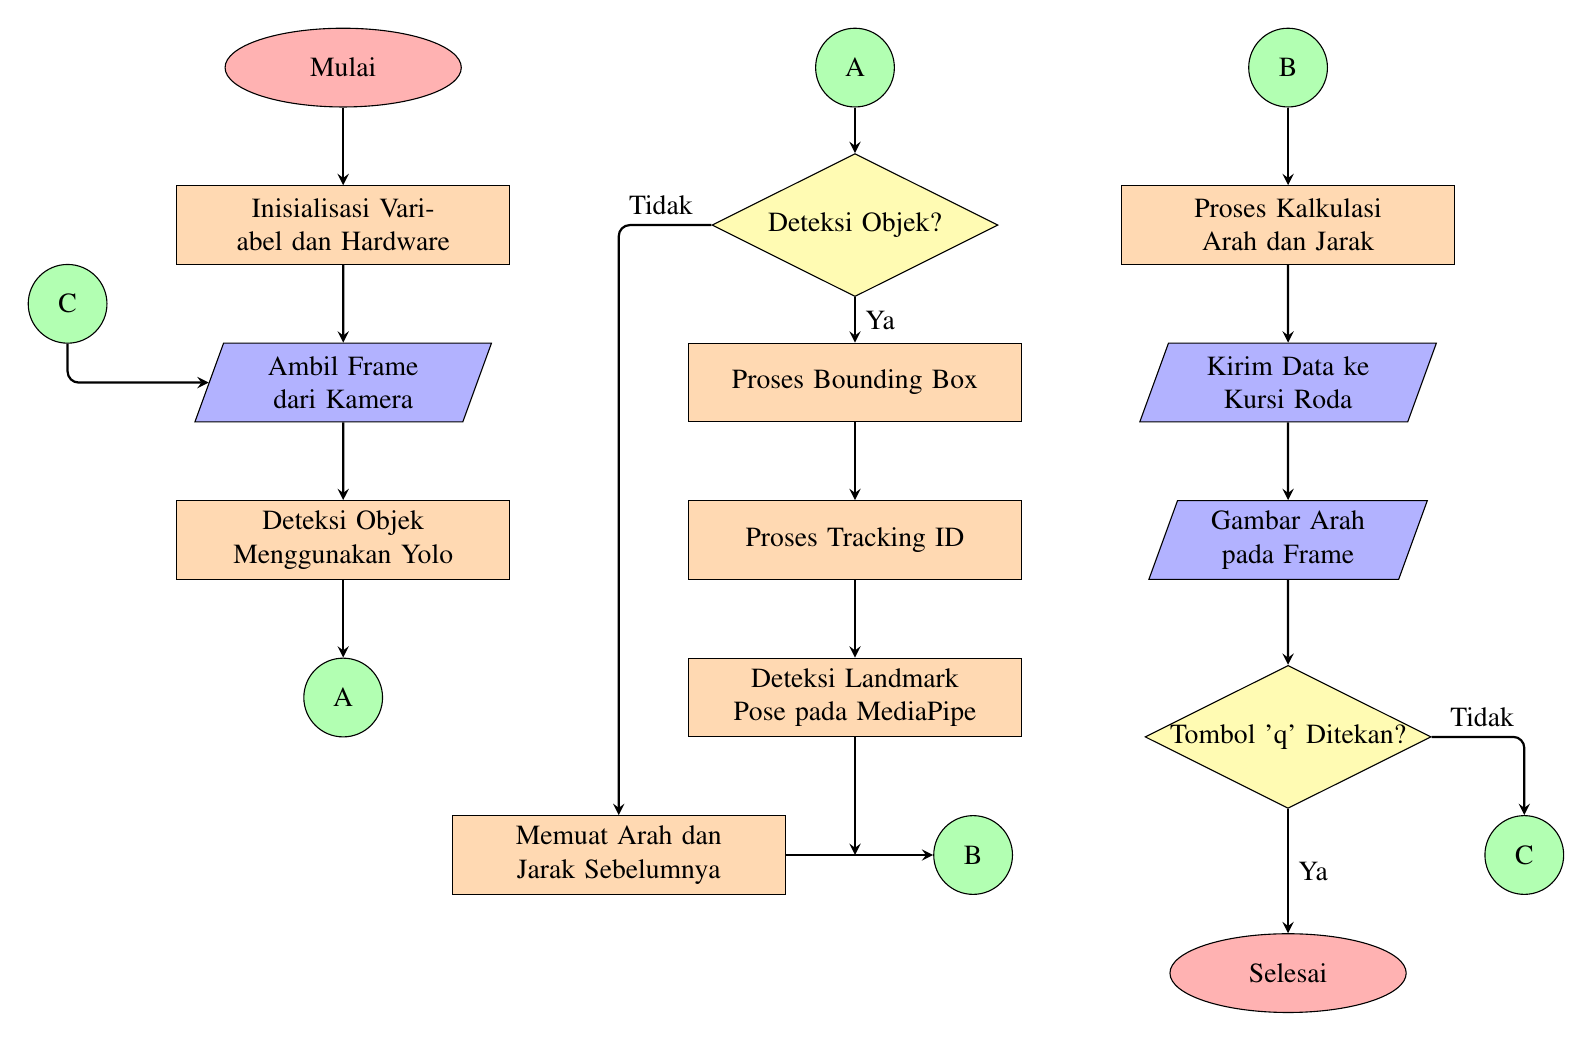
\begin{tikzpicture}[node distance=2cm]
      \node (start) [startstop] {Mulai};
      \node (initVars) [process, below of=start] {Inisialisasi Variabel dan Hardware};
      \node (captureFrame) [io, below of=initVars] {Ambil Frame dari Kamera};
      \node (yoloDetect) [process, below of=captureFrame] {Deteksi Objek Menggunakan Yolo};
      \node (A) [connector, below of=yoloDetect] {A};
      \node (C0) [connector, left of=initVars, xshift=-1.5cm, yshift=-1cm] {C};
  
      \node (A0) [connector, right of=start, xshift=4.5cm] {A};
      \node (checkBoxes) [decision, below of=A0] {Deteksi Objek?};
      \node (processBox) [process, below of=checkBoxes] {Proses Bounding Box};
      \node (trackingID) [process, below of=processBox] {Proses Tracking ID};
      \node (mediapipeProcessing) [process, below of=trackingID] {Deteksi Landmark Pose pada MediaPipe};
      \node (B) [connector, below of=mediapipeProcessing, xshift=1.5cm] {B};
  
      \node (B0) [connector, right of=A0, xshift=3.5cm] {B};
      \node (calcDirection) [process, below of=B0] {Proses Kalkulasi Arah dan Jarak};
      \node (controlWheelchair) [io, below of=calcDirection] {Kirim Data ke Kursi Roda};
      \node (display) [io, below of=controlWheelchair] {Gambar Arah pada Frame};
      \node (endLoop) [decision, below of=display, yshift=-.5cm] {Tombol 'q' Ditekan?};
      \node (C) [connector, right of=endLoop, xshift=1cm, yshift=-1.5cm] {C};
      \node (end) [startstop, below of=endLoop, yshift=-1cm] {Selesai};
  
      \node (searchPerson) [process, below of=mediapipeProcessing, xshift=-3cm] {Memuat Arah dan Jarak Sebelumnya};
      
      \draw [arrow] (start) -- (initVars);
      \draw [arrow] (initVars) -- (captureFrame);
      \draw [arrow] (captureFrame) -- (yoloDetect);
      \draw [arrow] (yoloDetect) -- (A);
      \draw [arrow] (C0) |- (captureFrame);
  
      \draw [arrow] (A0) -- (checkBoxes);
      \draw [arrow] (checkBoxes) -- node[anchor=west] {Ya} (processBox);
      \draw [arrow] (processBox) -- (trackingID);
      \draw [arrow] (trackingID) -- (mediapipeProcessing);
      \draw [arrow] (mediapipeProcessing) -- +(0,-2cm);
  
      \draw [arrow] (B0) -- (calcDirection);
      \draw [arrow] (calcDirection) -- (controlWheelchair);
      \draw [arrow] (controlWheelchair) -- (display);
      \draw [arrow] (display) -- (endLoop);
      \draw [arrow] (endLoop) -| node[anchor=south east] {Tidak} (C);
      \draw [arrow] (endLoop) -- node[anchor=west] {Ya} (end);
      
      \draw [arrow] (checkBoxes) -| node[anchor=south west] {Tidak} (searchPerson);
      \draw [arrow] (searchPerson) -- (B);
    \end{tikzpicture}
  }
  \caption{Flowchart program python}
\end{figure}

Program kemudian menghitung arah dan jarak target, yang digunakan untuk menentukan instruksi pergerakan kursi roda. Instruksi tersebut dikirimkan ke ESP32, yang mengendalikan motor kursi roda untuk mengikuti manusia secara otomatis. Selain itu, arah pergerakan digambarkan pada frame video yang ditampilkan sebagai bentuk visualisasi dari proses yang sedang berjalan. Program akan terus melakukan loop, menangkap gambar baru, memproses deteksi, dan mengirimkan perintah hingga pengguna menekan tombol 'q' untuk mengakhiri program.

\begin{figure}[H]
  \centering
  \resizebox{0.9\linewidth}{!}{
  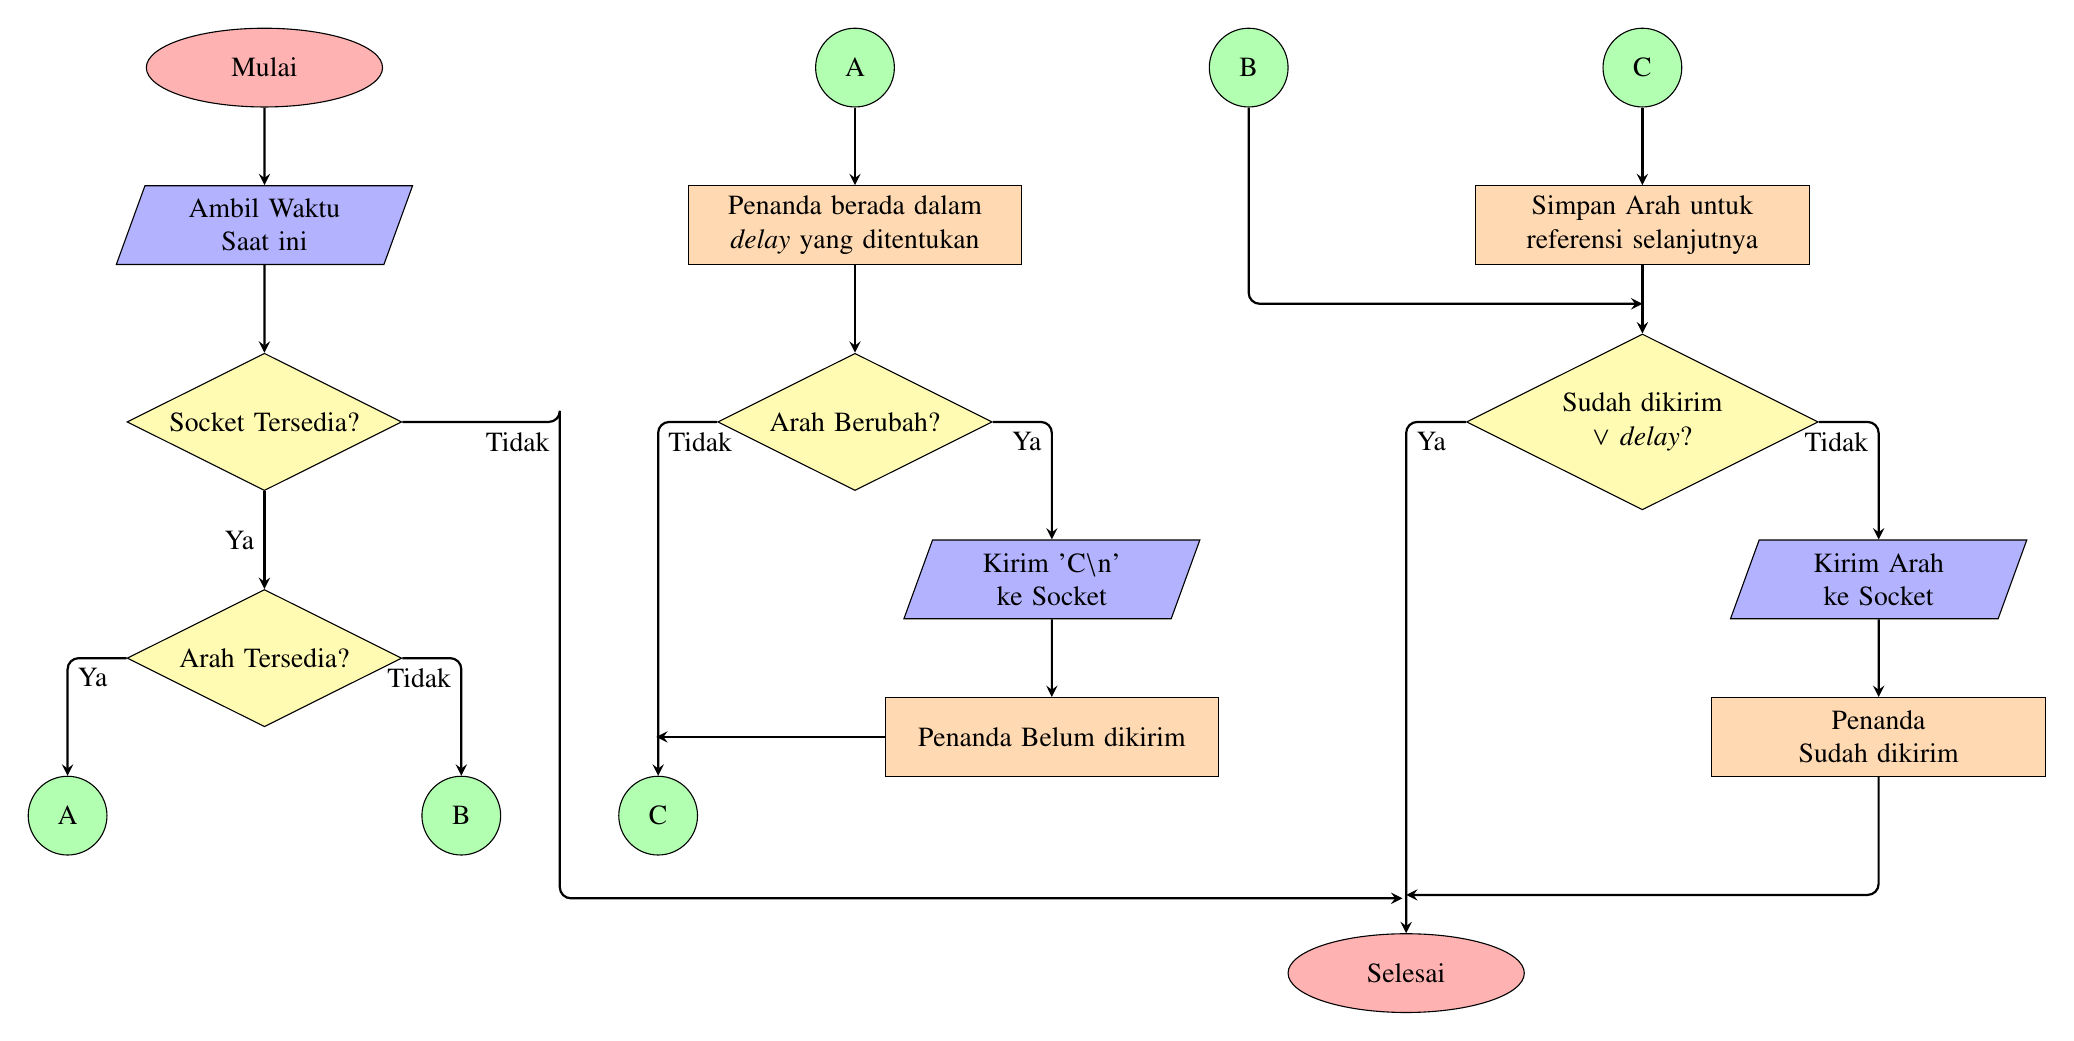
\begin{tikzpicture}[node distance=2cm]

    \node (start) [startstop] {Mulai};
    \node (getCurrentTime) [io, below of=start] {Ambil Waktu\\Saat ini};
    \node (checkSocket) [decision, below of=getCurrentTime, yshift=-.5cm] {Socket Tersedia?};
    \node (checkData) [decision, below of=checkSocket, yshift=-1cm] {Arah Tersedia?};
    \node (A) [connector, below of=checkData, xshift=-2.5cm] {A};
    \node (B) [connector, below of=checkData, xshift=2.5cm] {B};

    \node (A0) [connector, right of=start, xshift=5.5cm] {A};
    \node (setTime) [process, below of=A0] {Penanda berada dalam \emph{delay} yang ditentukan};
    \node (compareData) [decision, below of=setTime, yshift=-.5cm] {Arah Berubah?};
    \node (sendC) [io, below of=compareData, xshift=2.5cm] {Kirim 'C\textbackslash n' \\ke Socket};
    \node (setSentFalse) [process, below of=sendC] {Penanda Belum dikirim};
    \node (C) [connector, below of=setSentFalse, xshift=-5cm, yshift=1cm] {C};

    \node (B0) [connector, right of=A0, xshift=3cm] {B};

    \node (C0) [connector, right of=B0, xshift=3cm] {C};
    \node (setData) [process, below of=C0] {Simpan Arah untuk referensi selanjutnya};
    \node (checkInterval) [decision, below of=setData, yshift=-.5cm] {Sudah dikirim \(\lor\) \emph{delay}?};
    \node (sendData) [io, below of=checkInterval, xshift=3cm] {Kirim Arah \\ke Socket};
    \node (setSentTrue) [process, below of=sendData] {Penanda \\Sudah dikirim};
    \node (end) [startstop, below of=setSentTrue, xshift=-6cm, yshift=-1cm] {Selesai};
    
    \draw [arrow] (start) -- (getCurrentTime);
    \draw [arrow] (getCurrentTime) -- (checkSocket);
    \draw [arrow] (checkSocket) -- node[anchor=east] {Ya} (checkData);
    \draw [arrow] (checkData) -| node[anchor=north west] {Ya} (A);
    \draw [arrow] (checkData) -| node[anchor=north east] {Tidak} (B);

    \draw [arrow] (A0) -- (setTime);
    \draw [arrow] (setTime) -- (compareData);
    \draw [arrow] (compareData) -| node[anchor=north east] {Ya} (sendC);
    \draw [arrow] (sendC) -- (setSentFalse);
    \draw [arrow] (compareData) -| node[anchor=north west] {Tidak} (C);
    \draw [arrow] (setSentFalse.west) -- +(-2.9cm,0);

    \draw [arrow] (C0) -- (setData);
    \draw [arrow] (setData) -- (checkInterval);
    \draw [arrow] (checkInterval) -| node[anchor=north east] {Tidak} (sendData);
    \draw [arrow] (checkInterval) -| node[anchor=north west] {Ya} (end);
    \draw [arrow] (sendData) -- (setSentTrue);
    \draw [arrow] (setSentTrue.south) |- +(-6cm,-1.5cm);

    \draw [arrow] (B0) |- +(5cm,-3cm);
    \draw [arrow] (checkSocket.east) -| node[anchor=north east] {Tidak} +(2cm,0) |-  +(12.7cm,-6.05cm);
  
  \end{tikzpicture}
  }
  \caption{Flowchart regulasi arah}
\end{figure}

Regulasi arah kursi roda dilakukan melalui pengiriman data arah ke socket yang berhubungan dengan ESP32. Program mengecek apakah socket tersedia dan apakah data arah berubah, serta menetapkan penanda untuk menghindari pengiriman data yang berulang. Sebelum arah diubah, data 'C\textbackslash n' dikirim terlebih dahulu untuk memastikan kursi roda berhenti dan stabil sebelum menerima instruksi arah baru. Hal ini penting untuk mencegah gerakan yang tidak diinginkan atau perubahan arah yang terlalu mendadak. Setiap kali arah berubah setelah berhenti, data baru akan dikirim ke socket untuk mengontrol motor kursi roda.

Untuk ESP32 CAM, sistem dimulai dengan inisialisasi kamera yang terhubung ke ESP32. Langkah pertama adalah pengaturan kamera agar siap menangkap gambar lingkungan secara real-time. Kamera yang digunakan adalah OV5640 dengan resolusi 5MP, yang memungkinkan pengambilan gambar berkualitas tinggi untuk deteksi yang lebih akurat.

\begin{figure}[H]
  \centering
  \resizebox{0.7\linewidth}{!}{
  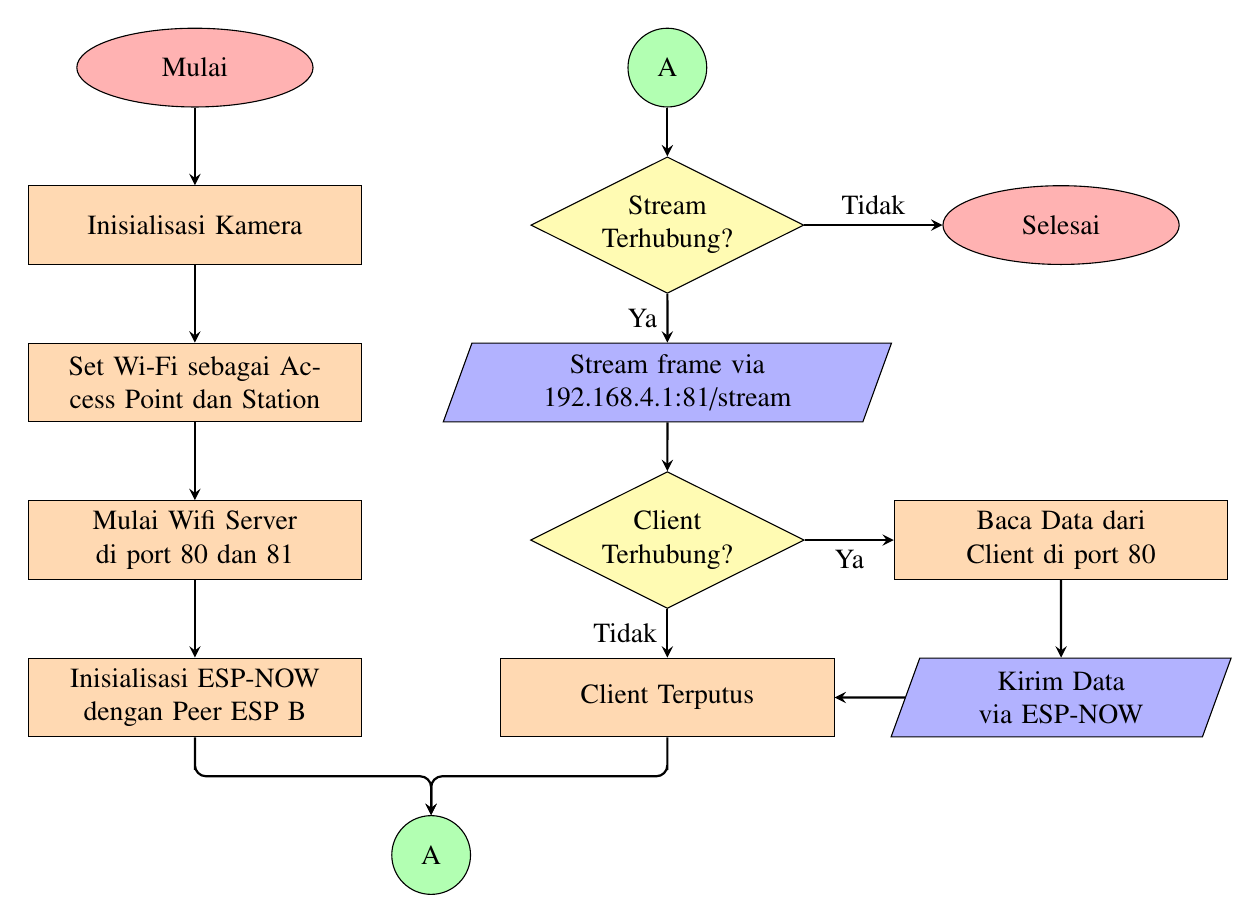
\begin{tikzpicture}[node distance=2cm]
    \node (start) [startstop] {Mulai};
    \node (camera) [process, below of=start] {Inisialisasi Kamera};
    \node (wifi) [process, below of=camera] {Set Wi-Fi sebagai Access Point dan Station};
    \node (server) [process, below of=wifi] {Mulai Wifi Server di port 80 dan 81};
    \node (espNow) [process, below of=server] {Inisialisasi ESP-NOW dengan Peer ESP B};
    \node (A) [connector, below of=espNow, xshift=3cm] {A};

    \node (A0) [connector, right of=start, xshift=4cm] {A};
    \node (stream) [decision, below of=A0, text width=2cm] {Stream Terhubung?};
    \node (peer) [io, below of=stream, text width=4.5cm] {Stream frame via 192.168.4.1:81/stream};
    \node (client) [decision, below of=peer, text width=2cm] {Client Terhubung?};
    \node (readData) [process, right of=client, xshift=3cm] {Baca Data dari Client di port 80};
    \node (sendESPNow) [io, below of=readData, text width=3cm] {Kirim Data via ESP-NOW};
    \node (clientStop) [process, below of=client] {Client Terputus};

    \node (stop) [startstop, right of=stream, xshift=3cm] {Selesai};

    % Arrows
    \draw [arrow] (start) -- (camera);
    \draw [arrow] (camera) -- (wifi);
    \draw [arrow] (wifi) -- (server);
    \draw [arrow] (server) -- (espNow);
    \draw [arrow] (espNow) |- ++(0,-1cm) -| (A);

    \draw [arrow] (A0) -- (stream);
    \draw [arrow] (stream) -- node[anchor=south] {Tidak} (stop);
    \draw [arrow] (stream) -- node[anchor=east] {Ya} (peer);
    \draw [arrow] (peer) -- (client);

    \draw [arrow] (client) -- node[anchor=north] {Ya} (readData);
    \draw [arrow] (client) -- node[anchor=east] {Tidak} (clientStop);
    \draw [arrow] (readData) -- (sendESPNow);
    \draw [arrow] (sendESPNow) -- (clientStop);
    \draw [arrow] (clientStop) |- ++(0,-1cm) -| (A);
  \end{tikzpicture}
  }
  \caption{Flowchart ESP A}
\end{figure}

Setelah inisialisasi kamera, sistem kemudian mengatur ESP32 untuk berfungsi sebagai WiFi Access Point. Pengaturan ini memungkinkan ESP32 menciptakan jaringan WiFi yang dapat digunakan untuk berkomunikasi dengan perangkat lain. Server WiFi diatur pada port 80 untuk menerima permintaan data dan port 81 untuk melakukan streaming data video secara real-time. Dengan streaming ini, gambar yang ditangkap oleh kamera dapat langsung diakses dan dianalisis oleh unit kontrol.

Setelah WiFi dan server diinisialisasi, ESP-NOW digunakan untuk komunikasi antara kedua ESP32. ESP-NOW adalah protokol komunikasi peer-to-peer yang memungkinkan transmisi data antar perangkat ESP32 tanpa memerlukan jaringan WiFi eksternal. Hal ini sangat penting karena memungkinkan komunikasi data yang cepat dan efisien antara ESP32 yang terhubung ke kamera (ESP32 A) dan ESP32 yang bertanggung jawab atas kontrol motor (ESP32 B). ESP-NOW memiliki latensi rendah, sehingga sangat cocok untuk aplikasi real-time seperti ini.

Dengan menggunakan protokol ESP-NOW, data yang ditangkap oleh kamera pada ESP32 A dapat langsung diteruskan ke ESP32 B tanpa keterlambatan. Protokol ini juga lebih hemat daya dibandingkan menggunakan jaringan WiFi umum, sehingga sangat cocok untuk aplikasi mobile seperti kursi roda otonom. Kombinasi dari server WiFi untuk streaming data dan ESP-NOW untuk transmisi instruksi memastikan bahwa sistem dapat mengirim dan menerima data dengan cepat, menjaga kursi roda tetap sinkron dengan pergerakan target manusia.

Selain itu, penggunaan server WiFi memungkinkan unit kontrol (seperti komputer atau laptop) mengakses data gambar secara langsung melalui jaringan lokal. Hal ini sangat berguna untuk menganalisis gambar secara lebih rinci dan mengambil keputusan kontrol yang lebih kompleks, seperti perubahan arah atau kecepatan kursi roda berdasarkan posisi target dalam frame. Dengan demikian, proses ini memberikan fleksibilitas yang tinggi dalam mengatur pergerakan kursi roda berdasarkan data yang diperoleh dari kamera.

Frame yang ditangkap oleh kamera dikirim melalui alamat IP tertentu yang juga digunakan dalam kode program Python untuk melakukan streaming data. Data arah yang diterima dari client kemudian diteruskan ke ESP32 B melalui ESP-NOW untuk mengontrol kursi roda. Sistem ini dirancang untuk memastikan komunikasi yang cepat dan handal antara ESP32 A dan ESP32 B, sehingga kursi roda dapat merespons pergerakan target dengan tepat.

\begin{figure}[H]
  \centering
  \resizebox{0.7\linewidth}{!}{
  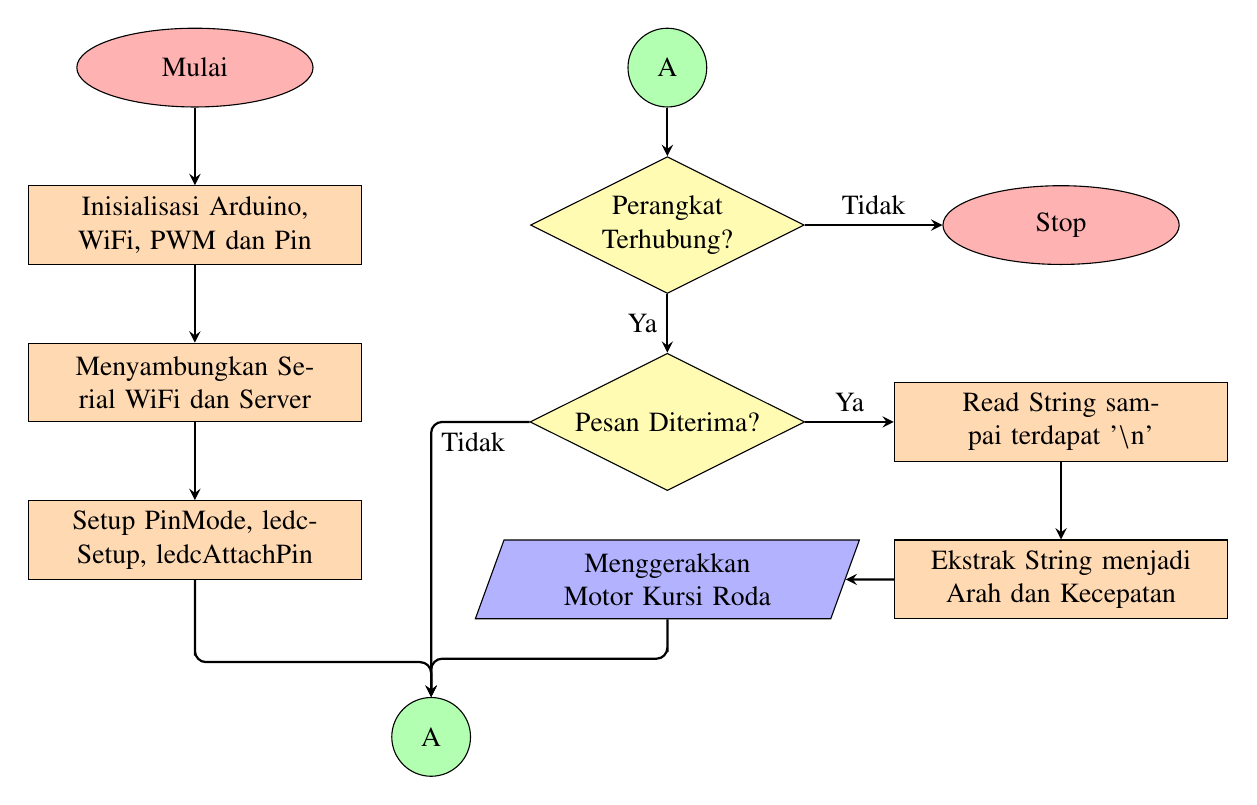
\begin{tikzpicture}[node distance=2cm]
    % Nodes
    \node (start) [startstop] {Mulai};
    \node (init) [process, below of=start] {Inisialisasi Arduino, WiFi, PWM dan Pin};
    \node (connect) [process, below of=init] {Menyambungkan Serial WiFi dan Server};
    \node (setup) [process, below of=connect] {Setup PinMode, ledc-Setup, ledcAttachPin};
    \node (A) [connector, below of=setup, xshift=3cm, yshift=-.5cm] {A};

    \node (A0) [connector, right of=start, xshift=4cm] {A};
    \node (connected?) [decision, below of=A0, text width=2cm] {Perangkat Terhubung?};
    \node (msg?) [decision, below of=connected?, yshift=-.5cm] {Pesan Diterima?};

    \node (stop) [startstop, right of=connected?, xshift=3cm] {Stop};
    \node (readstr) [process, right of=msg?, xshift=3cm] {Read String sampai terdapat '\textbackslash n'};
    \node (extract) [process, below of=readstr] {Ekstrak String menjadi Arah dan Kecepatan};
    \node (move) [io, below of=msg?, text width=3.5cm] {Menggerakkan Motor Kursi Roda};


    % Arrows
    \draw [arrow] (start) -- (init);
    \draw [arrow] (init) -- (connect);
    \draw [arrow] (connect) -- (setup);
    \draw [arrow] (setup) |- ++(0,-1.55cm) -| (A);

    \draw [arrow] (A0) -- (connected?);
    \draw [arrow] (connected?) -- node[anchor=east] {Ya} (msg?);
    \draw [arrow] (connected?) -- node[anchor=south] {Tidak} (stop);
    \draw [arrow] (msg?) -- node[anchor=south] {Ya} (readstr);
    \draw [arrow] (msg?.west) -| node[anchor=north west] {Tidak} (A);
    \draw [arrow] (readstr) -- (extract);
    \draw [arrow] (extract) -- (move);
    \draw [arrow] (move.south) |- ++(0,-.5) -| (A);
  \end{tikzpicture}
  }
  \caption{Flowchart ESP B}
\end{figure}

Pada sisi ESP32 Motor, perangkat dimulai dengan inisialisasi berbagai komponen, seperti PWM, WiFi, dan pin untuk mengendalikan motor. Setelah terhubung ke WiFi, ESP32 B menunggu pesan dari server yang berfungsi sebagai pusat kendali. Jika pesan diterima, string yang mengandung informasi arah dan kecepatan akan diekstrak, kemudian diolah untuk menentukan pergerakan motor kursi roda. Sistem menggunakan data ini untuk mengatur arah dan kecepatan motor, yang memastikan kursi roda dapat mengikuti target secara akurat dan responsif. Proses ini dilakukan secara berulang untuk setiap update data yang diterima, memungkinkan kursi roda menyesuaikan gerakan dengan perubahan posisi target secara real-time.

\cleardoublepage

% Bab 4 pengujian dan analisis
\chapter{PENGUJIAN DAN ANALISIS}
\label{chap:pengujiananalisis}

% Ubah bagian-bagian berikut dengan isi dari pengujian dan analisis

Pada bab ini, akan dijelaskan mengenai hasil pengujian dan pembahasan dari penelitian yang telah diuraikan pada metodologi. Selain itu, akan dipaparkan juga mengenai skenario pengujian yang dilakukan untuk mengevaluasi performa sistem secara keseluruhan. Pengujian ini dilakukan dengan tujuan untuk memastikan bahwa sistem yang dirancang mampu berfungsi dengan baik dalam berbagai kondisi dan situasi yang mungkin dihadapi dalam penggunaannya.

\section{Skenario Pengujian}
\label{sec:skenariopengujian}

Pengujian dilakukan untuk mengetahui performa model dalam melakukan deteksi dan mengikuti objek oleh kursi roda otonom. Skenario pengujian ini dirancang untuk mengukur berbagai aspek dari sistem, termasuk akurasi deteksi, kecepatan pemrosesan, respons sistem terhadap objek, dan tingkat keberhasilan mengidentifikasi tracking. Skenario pengujian yang akan dilakukan adalah sebagai berikut:

\begin{enumerate}
    \item Hasil Pengujian Performa Model
    \item Pengujian Berdasarkan FPS
    \item Pengujian Berdasarkan Hasil Response Time
    \item Pengujian Keberhasilan Tracking
    \item Pengujian Tingkat Pencahayaan
    \item Pengujian Kesesuaian Jarak Deteksi
    \item Performa Pergerakan Mengikuti Objek
    \item Performa Keberhasilan Mengikuti Objek
\end{enumerate}

\newpage
\section{Hasil Pengujian Performa Menggunakan Confusion Matrix}
\label{sec:hasilperformaconfisionMatrix}

Sebanyak 15163 citra manusia dan 590 data validasi digunakan sebagai data latih awal. Melalui proses augmentasi, jumlah data latih meningkat menjadi 4.359, sementara data validasi bertambah menjadi 1.023. Setelah jumlah dataset ditentukan, langkah selanjutnya adalah membuat API key pada Roboflow yang kemudian diintegrasikan untuk proses pelatihan model.

Proses pelatihan model dimulai setelah seluruh dataset dimuat. Selama pelatihan, beberapa parameter digunakan dan hasilnya dibandingkan menggunakan nilai confusion matrix serta metrik akurasi deteksi seperti mAP score, precision, dan box loss. Layer input pertama dijelaskan sebagai tahap awal pelatihan model.

Pelatihan dilakukan selama 100 epoch pertama dengan ukuran batch sebesar 16 piksel, dan data diubah ukurannya menjadi 800 x 800 piksel selama preprocessing. Tujuan dari pelatihan ini adalah untuk mengevaluasi seberapa besar peningkatan performa model terlatih sebelumnya dalam mendeteksi manusia berdasarkan jumlah epoch yang dilakukan. Pada akhir 100 epoch, nilai box loss yang dihasilkan adalah 0,82978, yang menunjukkan kemampuan model untuk memprediksi bounding box dengan baik di sekitar objek. Penurunan nilai box loss selama pelatihan menunjukkan bahwa model berhasil belajar mengidentifikasi koordinat bounding box secara akurat.

Selama validasi, nilai box loss tercatat sebesar 1,199, yang mengindikasikan kemampuan model dalam mengenali objek pada data uji. Penurunan box loss pada tahap validasi mencerminkan kemampuan model untuk mendeteksi objek secara general, tidak hanya pada data latih. Nilai mAP score divisualisasikan pada Gambar, dengan hasil skor mAP sebesar 81,85% untuk IoU minimum 0,5, yang menegaskan akurasi tinggi dalam mendeteksi objek.

Secara keseluruhan, hasil pelatihan model dirangkum pada Gambar. Nilai box loss pada pelatihan adalah 0,82978, nilai cls loss adalah 0,57615, dan dfl loss sebesar 1,1197. Metrik lainnya meliputi precision (0,84974), recall (0,72608), mAP50 (0,81855), dan mAP50-95 (0,53527). Selama validasi, nilai box loss tercatat sebesar 1,199, cls loss sebesar 0,86314, dan dfl loss sebesar 1,4956.

Visualisasi hasil model disajikan melalui confusion matrix yang menggambarkan kinerja deteksi secara rinci. Matrix ini menunjukkan 1.806 data sebagai True Positive (manusia terdeteksi dengan benar), 483 data sebagai False Positive (objek salah terdeteksi sebagai manusia), dan 475 data sebagai False Negative (manusia yang tidak terdeteksi).

Kurva F1-Confidence yang dihasilkan selama pelatihan menunjukkan hubungan antara confidence score dan F1-score. Model mencapai nilai F1-score tertinggi sebesar 0,78 pada confidence score 0,450, mengindikasikan keseimbangan optimal antara precision dan recall. Namun, kurva menunjukkan penurunan signifikan setelah confidence score mencapai sekitar 0,8, yang menandakan bahwa pada tingkat confidence yang sangat tinggi, model cenderung mengabaikan banyak true positives, sehingga menurunkan F1-score keseluruhan.

Inferensi terhadap data uji juga dilakukan menggunakan model yang telah dilatih. Hasilnya menunjukkan tingkat confidence yang tinggi pada deteksi objek manusia, sebagaimana divisualisasikan dalam gambar hasil pengujian

\section{Pengujian Berdasarkan FPS}
\label{sec:pengujianberdasarkanfps}

Pengujian ini dilakukan untuk menganalisis kecepatan pemrosesan sistem dalam satuan Frame per Second (FPS). FPS yang tinggi menunjukkan bahwa sistem dapat bekerja dengan baik secara real-time. Grafik hasil pengujian disertakan untuk memudahkan visualisasi performa.

\section{Pengujian Berdasarkan Response Time}
\label{sec:pengujianberdasarkanresponsetime}

Bagian ini mengukur waktu yang dibutuhkan sistem untuk merespons setiap perubahan lingkungan atau perintah yang diterima. Response Time sangat penting untuk mengukur responsivitas sistem dalam skenario dinamis.

\section{Pengujian Keberhasilan Tracking}
\label{sec:pengujiankeberhasiltracking}

Bagian ini mengevaluasi keberhasilan sistem dalam melakukan tracking terhadap objek target. Tingkat keberhasilan dianalisis untuk mengetahui keandalan sistem dalam berbagai skenario.

\section{Pengujian Tingkat Pencahayaan}
\label{sec:pengujiantingkatpencahayaan}

Pengujian dilakukan untuk mengukur kemampuan sistem dalam mendeteksi objek pada berbagai tingkat pencahayaan. Fokus pengujian ini adalah memastikan bahwa sistem dapat berfungsi dengan baik dalam kondisi pencahayaan yang berbeda.

\newpage
\section{Pengujian Kesesuaian Jarak Deteksi}
\label{sec:pengujiankesesuaianjarakdeteksi}

Pengujian dilakukan untuk mengukur kemampuan sistem dalam mendeteksi objek pada berbagai jarak dan menganalisis performa sistem pada jarak-jarak tersebut. Fokus pengujian ini adalah memastikan bahwa ketika objek berada pada jarak yang sangat dekat (\textless 1m), sistem mengirimkan kode instruksi untuk berhenti (diam) guna mencegah tabrakan.

\begin{table}[H]
    \centering
    \caption{Data Jarak (\textless 1m) untuk Diam}
    \label{tab:jarak_diam}
    \begin{tabular}{|c|c|c|c|c|c|c|c|c|}
    \hline
    Waktu & Reg (s) & YOLO (m) & MP (m) & x (px) & Deteksi & Terkirim & Keterangan \\ \hline
    12:55:12 & 0.8402 & 2.0631 & 0.9852 & 833 & b'C\textbackslash n' & b'C\textbackslash n' & Stop \\ \hline
    12:55:15 & 0.2585 & 1.1003 & 0.8942 & 242 & b'C\textbackslash n' & b'C\textbackslash n' & Stop \\ \hline
    12:55:24 & 2.1821 & 1.1773 & 0.9652 & 511 & b'C\textbackslash n' & b'C\textbackslash n' & Stop \\ \hline
    12:58:13 & 1.4998 & 1.4123 & 0.9574 & 531 & b'C\textbackslash n' & b'C\textbackslash n' & Stop \\ \hline
    12:58:14 & 0.2538 & 1.4538 & 0.9899 & 555 & b'C\textbackslash n' & b'C\textbackslash n' & Stop \\ \hline
    12:58:19 & 2.4033 & 1.1691 & 0.9213 & 852 & b'C\textbackslash n' & b'C\textbackslash n' & Stop \\ \hline
    12:58:19 & 0.4079 & 1.1839 & 0.9118 & 854 & b'C\textbackslash n' & b'C\textbackslash n' & Stop \\ \hline
    12:58:20 & 0.8708 & 1.0960 & 0.9548 & 528 & b'C\textbackslash n' & b'C\textbackslash n' & Stop \\ \hline
    12:58:21 & 0.4262 & 1.1003 & 0.9189 & 547 & b'C\textbackslash n' & b'C\textbackslash n' & Stop \\ \hline
    12:58:21 & 0.3497 & 1.1032 & 0.8985 & 554 & b'C\textbackslash n' & b'C\textbackslash n' & Stop \\ \hline
    12:58:21 & 0.3314 & 1.1032 & 0.8785 & 518 & b'C\textbackslash n' & b'C\textbackslash n' & Stop \\ \hline
    13:00:57 & 1.4848 & 1.1594 & 0.9943 & 208 & b'C\textbackslash n' & b'C\textbackslash n' & Stop \\ \hline
    13:01:15 & 1.5987 & 1.3643 & 0.9899 & 849 & b'C\textbackslash n' & b'C\textbackslash n' & Stop \\ \hline
    13:01:19 & 0.2719 & 1.0989 & 0.7700 & 856 & b'C\textbackslash n' & b'C\textbackslash n' & Stop \\ \hline
    13:01:19 & 0.2509 & 1.1452 & 0.5782 & 856 & b'C\textbackslash n' & b'C\textbackslash n' & Stop \\ \hline
    17:41:34 & 0.3036 & 1.4339 & 0.9447 & 647 & b'C\textbackslash n' & b'C\textbackslash n' & Stop \\ \hline
    17:41:35 & 0.3326 & 1.4291 & 0.8357 & 642 & b'C\textbackslash n' & b'C\textbackslash n' & Stop \\ \hline
    17:41:36 & 0.3588 & 1.4389 & 0.8222 & 672 & b'C\textbackslash n' & b'C\textbackslash n' & Stop \\ \hline
    17:41:45 & 0.3092 & 1.3913 & 0.7249 & 640 & b'C\textbackslash n' & b'C\textbackslash n' & Stop \\ \hline
    17:42:04 & 15.5192 & 1.4563 & 0.5955 & 213 & b'C\textbackslash n' & b'C\textbackslash n' & Stop \\ \hline
    \end{tabular}
    \end{table}

Tabel \ref{tab:jarak_diam} menunjukkan data jarak yang diukur ketika objek berada pada jarak kurang dari 1 meter. Data ini mencakup waktu deteksi, jarak deteksi dari YOLOv11 dan MediaPipe Pose, posisi objek dalam frame, hasil deteksi, instruksi yang dikirimkan, dan keterangan mengenai status objek. Data ini memberikan gambaran kinerja sistem dalam mengikuti objek yang berada pada jarak dekat, termasuk kecepatan respons, akurasi deteksi, dan ketepatan instruksi yang dikirimkan.

Pengujian jarak juga telah diverifikasi secara fisik dengan pengukuran dan perbandingan yang cermat sebelum menyajikan data. Hal ini memastikan akurasi dan keandalan pengukuran jarak yang digunakan dalam evaluasi. Proses verifikasi melibatkan penggunaan alat ukur yang terkalibrasi dan uji coba berulang untuk meminimalkan kesalahan.

\newpage
\section{Performa Pergerakan Mengikuti Objek}
\label{sec:performaakurasiobjek}

Analisis dilakukan untuk mengukur seberapa akurat sistem dapat mengikuti objek target, termasuk mempertahankan jarak yang tepat dan tidak kehilangan objek dalam berbagai kondisi.

\subsection{Percobaan Dalam Frame}
\label{subsec:percobaandalamframe}

Bagian ini membahas kemampuan sistem dalam mengikuti objek yang berada di dalam frame kamera dengan fokus utama pada evaluasi kinerja regulator. Tujuannya adalah memastikan bahwa sistem dapat merespons hasil deteksi dengan akurat dan konsisten, sesuai dengan kondisi objek yang terdeteksi di dalam frame kamera. Analisis dilakukan menggunakan 100 data sampel untuk memberikan gambaran kinerja sistem secara menyeluruh.

\begin{longtable}{|c|c|c|c|c|c|c|c|}
    \caption{Data Status Frame (Dalam Frame)} \label{tab:status_dalam_frame} \\
    \hline
    Waktu & Reg (s) & YOLO (m) & MP (m) & x (px) & Deteksi & Terkirim & Keterangan \\ \hline
    \endhead
    \hline \multicolumn{8}{|r|}{Lanjutan ke halaman berikutnya} \\ \hline
    \endfoot
    \endlastfoot
    12:48:09 & 0.2960 & 2.4469 & 2.6214 & 765 & b'E\textbackslash n' & b'C\textbackslash n' & Turn Right \\ \hline
12:48:09 & 0.2991 & 5.6875 & 4.1146 & 484 & b'B\textbackslash n' & b'E\textbackslash n' & Forward \\ \hline
12:48:10 & 0.2516 & 2.2093 & 2.6063 & 595 & b'B\textbackslash n' & b'C\textbackslash n' & Forward \\ \hline
12:48:14 & 2.7739 & 1.4513 & 1.7409 & 128 & b'A\textbackslash n' & b'A\textbackslash n' & Turn Left \\ \hline
12:48:17 & 2.6621 & 1.7109 & 1.1479 & 447 & b'B\textbackslash n' & b'C\textbackslash n' & Forward \\ \hline
12:50:45 & 0.5046 & 2.5900 & 1.4523 & 391 & b'B\textbackslash n' & b'B\textbackslash n' & Forward \\ \hline
12:50:48 & 2.7333 & 1.1421 & 1.9733 & 164 & b'A\textbackslash n' & b'C\textbackslash n' & Turn Left \\ \hline
12:50:51 & 0.4610 & 1.4219 & 1.0142 & 830 & b'E\textbackslash n' & b'E\textbackslash n' & Turn Right \\ \hline
12:50:54 & 2.5388 & 1.4768 & 1.1208 & 501 & b'B\textbackslash n' & b'C\textbackslash n' & Forward \\ \hline
12:50:57 & 0.2675 & 2.0939 & 1.4524 & 825 & b'E\textbackslash n' & b'E\textbackslash n' & Turn Right \\ \hline
12:51:00 & 0.3556 & 1.7144 & 1.5984 & 492 & b'B\textbackslash n' & b'C\textbackslash n' & Forward \\ \hline
12:51:00 & 0.3290 & 1.4978 & 1.4964 & 466 & b'B\textbackslash n' & b'B\textbackslash n' & Forward \\ \hline
12:51:07 & 3.9922 & 1.7796 & 1.3830 & 896 & b'E\textbackslash n' & b'C\textbackslash n' & Turn Right \\ \hline
12:51:08 & 0.3129 & 1.6801 & 1.7017 & 525 & b'B\textbackslash n' & b'C\textbackslash n' & Forward \\ \hline
12:51:09 & 0.3226 & 1.6408 & 1.7256 & 463 & b'B\textbackslash n' & b'B\textbackslash n' & Forward \\ \hline
12:51:11 & 2.3641 & 1.5332 & 1.1242 & 850 & b'E\textbackslash n' & b'C\textbackslash n' & Turn Right \\ \hline
12:51:17 & 5.5467 & 2.2628 & 1.6525 & 563 & b'B\textbackslash n' & b'C\textbackslash n' & Forward \\ \hline
12:51:17 & 0.3035 & 1.9853 & 1.6709 & 408 & b'B\textbackslash n' & b'B\textbackslash n' & Forward \\ \hline
12:51:18 & 0.3176 & 1.6668 & 1.5184 & 189 & b'A\textbackslash n' & b'C\textbackslash n' & Turn Left \\ \hline
12:51:18 & 0.3818 & 1.5277 & 1.4295 & 202 & b'A\textbackslash n' & b'A\textbackslash n' & Turn Left \\ \hline
12:51:21 & 2.9916 & 2.0186 & 1.6728 & 440 & b'B\textbackslash n' & b'C\textbackslash n' & Forward \\ \hline
12:51:21 & 0.3446 & 2.4830 & 1.6701 & 601 & b'B\textbackslash n' & b'B\textbackslash n' & Forward \\ \hline
12:51:22 & 0.2721 & 2.6141 & 1.7926 & 769 & b'E\textbackslash n' & b'C\textbackslash n' & Turn Right \\ \hline
12:51:22 & 0.2947 & 2.7330 & 1.5570 & 867 & b'E\textbackslash n' & b'E\textbackslash n' & Turn Right \\ \hline
12:51:26 & 3.8579 & 2.5354 & 1.6134 & 553 & b'B\textbackslash n' & b'C\textbackslash n' & Forward \\ \hline
12:51:26 & 0.4472 & 1.9174 & 1.2873 & 212 & b'A\textbackslash n' & b'C\textbackslash n' & Turn Left \\ \hline
12:51:27 & 0.2536 & 1.6668 & 1.9112 & 142 & b'A\textbackslash n' & b'A\textbackslash n' & Turn Left \\ \hline
12:51:30 & 3.3993 & 2.4258 & 1.4468 & 551 & b'B\textbackslash n' & b'C\textbackslash n' & Forward \\ \hline
12:51:36 & 4.6957 & 1.7144 & 1.8941 & 478 & b'B\textbackslash n' & b'B\textbackslash n' & Forward \\ \hline
12:51:37 & 1.7377 & 1.5194 & 1.8537 & 182 & b'A\textbackslash n' & b'C\textbackslash n' & Turn Left \\ \hline
12:51:42 & 0.2820 & 1.4820 & 1.5157 & 424 & b'B\textbackslash n' & b'C\textbackslash n' & Forward \\ \hline
12:51:42 & 0.2867 & 1.5473 & 1.6206 & 481 & b'B\textbackslash n' & b'B\textbackslash n' & Forward \\ \hline
12:51:44 & 0.3591 & 2.1528 & 1.7878 & 245 & b'A\textbackslash n' & b'C\textbackslash n' & Turn Left \\ \hline
12:51:44 & 0.2619 & 1.6003 & 1.9633 & 426 & b'B\textbackslash n' & b'A\textbackslash n' & Forward \\ \hline
12:51:45 & 0.2692 & 1.5704 & 1.6022 & 449 & b'B\textbackslash n' & b'C\textbackslash n' & Forward \\ \hline
12:51:45 & 0.3616 & 1.8259 & 1.5129 & 249 & b'A\textbackslash n' & b'B\textbackslash n' & Turn Left \\ \hline
12:51:48 & 2.8133 & 1.7721 & 1.1400 & 766 & b'E\textbackslash n' & b'C\textbackslash n' & Turn Right \\ \hline
12:51:48 & 0.2701 & 1.9485 & 1.8638 & 792 & b'E\textbackslash n' & b'E\textbackslash n' & Turn Right \\ \hline
12:51:51 & 2.5508 & 2.2628 & 1.9379 & 569 & b'B\textbackslash n' & b'C\textbackslash n' & Forward \\ \hline
12:51:52 & 0.6972 & 1.9174 & 1.6452 & 394 & b'B\textbackslash n' & b'B\textbackslash n' & Forward \\ \hline
12:51:52 & 0.3755 & 1.5912 & 1.3909 & 185 & b'A\textbackslash n' & b'C\textbackslash n' & Turn Left \\ \hline
12:51:52 & 0.3613 & 1.4716 & 1.2101 & 174 & b'A\textbackslash n' & b'A\textbackslash n' & Turn Left \\ \hline
12:51:55 & 0.3125 & 1.9262 & 1.1721 & 564 & b'B\textbackslash n' & b'C\textbackslash n' & Forward \\ \hline
12:51:56 & 0.3797 & 1.9667 & 1.6343 & 835 & b'E\textbackslash n' & b'B\textbackslash n' & Turn Right \\ \hline
12:51:56 & 0.2506 & 1.9262 & 1.7147 & 880 & b'E\textbackslash n' & b'C\textbackslash n' & Turn Right \\ \hline
12:51:56 & 0.2716 & 1.9759 & 1.6276 & 871 & b'E\textbackslash n' & b'E\textbackslash n' & Turn Right \\ \hline
12:52:05 & 0.2830 & 1.9395 & 1.9075 & 502 & b'B\textbackslash n' & b'C\textbackslash n' & Forward \\ \hline
12:55:09 & 1.9217 & 1.5004 & 1.8914 & 861 & b'E\textbackslash n' & b'E\textbackslash n' & Turn Right \\ \hline
12:55:10 & 0.3128 & 1.4414 & 1.8698 & 858 & b'E\textbackslash n' & b'C\textbackslash n' & Turn Right \\ \hline
12:55:10 & 0.3967 & 1.7356 & 1.0821 & 856 & b'E\textbackslash n' & b'E\textbackslash n' & Turn Right \\ \hline
12:55:13 & 0.3498 & 2.0186 & 1.9290 & 520 & b'B\textbackslash n' & b'C\textbackslash n' & Forward \\ \hline
12:55:14 & 0.3321 & 1.8664 & 1.4010 & 511 & b'B\textbackslash n' & b'B\textbackslash n' & Forward \\ \hline
12:55:15 & 1.6785 & 1.1238 & 1.0672 & 170 & b'A\textbackslash n' & b'C\textbackslash n' & Turn Left \\ \hline
12:55:18 & 0.2536 & 1.2489 & 1.0783 & 483 & b'B\textbackslash n' & b'C\textbackslash n' & Forward \\ \hline
12:55:18 & 0.3224 & 1.2129 & 1.4666 & 168 & b'A\textbackslash n' & b'C\textbackslash n' & Turn Left \\ \hline
12:55:19 & 0.3399 & 1.1515 & 1.3422 & 165 & b'A\textbackslash n' & b'A\textbackslash n' & Turn Left \\ \hline
12:55:22 & 0.3309 & 1.5194 & 1.5842 & 504 & b'B\textbackslash n' & b'C\textbackslash n' & Forward \\ \hline
12:55:22 & 0.3887 & 1.4690 & 1.6042 & 528 & b'B\textbackslash n' & b'B\textbackslash n' & Forward \\ \hline
12:55:25 & 0.4715 & 1.1164 & 1.4924 & 170 & b'A\textbackslash n' & b'C\textbackslash n' & Turn Left \\ \hline
12:55:29 & 1.1263 & 1.4029 & 1.2103 & 509 & b'B\textbackslash n' & b'C\textbackslash n' & Forward \\ \hline
12:55:30 & 0.3296 & 1.4219 & 1.2387 & 508 & b'B\textbackslash n' & b'B\textbackslash n' & Forward \\ \hline
12:58:02 & 1.9436 & 1.2696 & 1.0367 & 149 & b'A\textbackslash n' & b'C\textbackslash n' & Turn Left \\ \hline
12:58:03 & 0.3955 & 1.0975 & 1.0832 & 145 & b'A\textbackslash n' & b'A\textbackslash n' & Turn Left \\ \hline
12:58:03 & 0.3395 & 1.6971 & 1.2674 & 619 & b'B\textbackslash n' & b'C\textbackslash n' & Forward \\ \hline
12:58:03 & 0.2777 & 1.6473 & 1.6845 & 616 & b'B\textbackslash n' & b'B\textbackslash n' & Forward \\ \hline
12:58:04 & 0.3573 & 1.4291 & 1.9911 & 795 & b'E\textbackslash n' & b'C\textbackslash n' & Turn Right \\ \hline
12:58:05 & 0.3560 & 1.6768 & 1.8145 & 795 & b'E\textbackslash n' & b'E\textbackslash n' & Turn Right \\ \hline
12:58:05 & 0.3549 & 1.3890 & 1.6223 & 130 & b'A\textbackslash n' & b'C\textbackslash n' & Turn Left \\ \hline
12:58:05 & 0.4054 & 1.3446 & 1.3906 & 174 & b'A\textbackslash n' & b'A\textbackslash n' & Turn Left \\ \hline
12:58:09 & 1.6364 & 1.4665 & 1.1057 & 425 & b'B\textbackslash n' & b'C\textbackslash n' & Forward \\ \hline
12:58:10 & 1.2931 & 1.4123 & 1.6479 & 320 & b'A\textbackslash n' & b'C\textbackslash n' & Turn Left \\ \hline
12:58:11 & 0.3293 & 1.2094 & 1.7544 & 445 & b'B\textbackslash n' & b'C\textbackslash n' & Forward \\ \hline
12:58:11 & 0.5372 & 1.2008 & 1.7284 & 503 & b'B\textbackslash n' & b'B\textbackslash n' & Forward \\ \hline
12:58:25 & 4.1776 & 1.1047 & 1.2300 & 197 & b'A\textbackslash n' & b'C\textbackslash n' & Turn Left \\ \hline
12:58:26 & 0.6310 & 1.1284 & 1.2368 & 195 & b'A\textbackslash n' & b'A\textbackslash n' & Turn Left \\ \hline
12:58:28 & 2.0228 & 1.3319 & 1.2516 & 442 & b'B\textbackslash n' & b'C\textbackslash n' & Forward \\ \hline
12:58:28 & 0.3156 & 1.3754 & 1.5678 & 432 & b'B\textbackslash n' & b'B\textbackslash n' & Forward \\ \hline
13:00:55 & 1.9408 & 1.0975 & 1.0855 & 185 & b'A\textbackslash n' & b'C\textbackslash n' & Turn Left \\ \hline
13:00:55 & 0.4380 & 1.0975 & 1.1142 & 177 & b'A\textbackslash n' & b'C\textbackslash n' & Turn Left \\ \hline
13:00:56 & 0.3263 & 1.0960 & 1.1078 & 167 & b'A\textbackslash n' & b'A\textbackslash n' & Turn Left \\ \hline
13:00:58 & 0.3332 & 1.3091 & 1.8538 & 444 & b'B\textbackslash n' & b'C\textbackslash n' & Forward \\ \hline
13:00:58 & 0.2737 & 1.6903 & 1.0003 & 215 & b'A\textbackslash n' & b'B\textbackslash n' & Turn Left \\ \hline
13:00:59 & 0.2535 & 1.6869 & 1.4439 & 228 & b'A\textbackslash n' & b'C\textbackslash n' & Turn Left \\ \hline
13:00:59 & 0.3323 & 1.7536 & 1.9650 & 225 & b'A\textbackslash n' & b'A\textbackslash n' & Turn Left \\ \hline
13:00:59 & 0.3355 & 1.4267 & 1.5125 & 456 & b'B\textbackslash n' & b'C\textbackslash n' & Forward \\ \hline
13:01:00 & 0.3113 & 1.2734 & 1.1814 & 173 & b'A\textbackslash n' & b'B\textbackslash n' & Turn Left \\ \hline
13:01:01 & 0.4180 & 1.6188 & 1.0805 & 170 & b'A\textbackslash n' & b'C\textbackslash n' & Turn Left \\ \hline
13:01:02 & 0.2600 & 1.5882 & 1.5507 & 222 & b'A\textbackslash n' & b'A\textbackslash n' & Turn Left \\ \hline
13:01:04 & 0.2826 & 1.3173 & 1.3641 & 483 & b'B\textbackslash n' & b'C\textbackslash n' & Forward \\ \hline
13:01:05 & 0.2677 & 1.3256 & 1.3744 & 534 & b'B\textbackslash n' & b'B\textbackslash n' & Forward \\ \hline
13:01:07 & 0.2501 & 1.1872 & 1.1742 & 513 & b'B\textbackslash n' & b'C\textbackslash n' & Forward \\ \hline
13:01:08 & 0.3496 & 1.3298 & 1.2935 & 499 & b'B\textbackslash n' & b'B\textbackslash n' & Forward \\ \hline
13:01:08 & 0.4923 & 1.6188 & 1.3519 & 211 & b'A\textbackslash n' & b'C\textbackslash n' & Turn Left \\ \hline
13:01:09 & 0.3287 & 1.7039 & 1.7476 & 202 & b'A\textbackslash n' & b'A\textbackslash n' & Turn Left \\ \hline
13:01:11 & 2.7773 & 1.5305 & 1.8361 & 517 & b'B\textbackslash n' & b'C\textbackslash n' & Forward \\ \hline
13:01:13 & 1.1224 & 1.8459 & 1.5848 & 850 & b'E\textbackslash n' & b'C\textbackslash n' & Turn Right \\ \hline
13:01:13 & 0.2936 & 1.5942 & 1.0293 & 832 & b'E\textbackslash n' & b'E\textbackslash n' & Turn Right \\ \hline
13:01:17 & 0.2969 & 1.1193 & 1.0841 & 540 & b'B\textbackslash n' & b'C\textbackslash n' & Forward \\ \hline
13:01:17 & 0.3835 & 1.1238 & 1.0723 & 862 & b'E\textbackslash n' & b'B\textbackslash n' & Turn Right \\ \hline
13:01:18 & 0.3058 & 1.1253 & 1.0494 & 845 & b'E\textbackslash n' & b'C\textbackslash n' & Turn Right \\ \hline
\end{longtable}

Tabel \ref{tab:status_dalam_frame} menunjukkan data status dalam frame selama pengujian. Data ini mencakup waktu deteksi, jarak deteksi dari YOLOv11 dan MediaPipe Pose, posisi objek dalam frame, hasil deteksi, instruksi yang dikirimkan, dan keterangan mengenai status objek. Data ini memberikan gambaran kinerja sistem dalam mengikuti objek yang berada di dalam frame kamera, termasuk kecepatan respons, akurasi deteksi, dan ketepatan instruksi yang dikirimkan.

Data yang terdapat pada tabel telah diolah dan ditampilkan dalam bentuk plot untuk mempermudah visualisasi hubungan antara waktu dan instruksi yang dikirimkan oleh sistem. Dengan memanfaatkan plot ini, pola serta tren dalam data dapat diamati secara lebih jelas, sehingga memberikan gambaran yang lebih komprehensif mengenai kinerja sistem selama pengujian.

\begin{figure}[H]
    \centering
    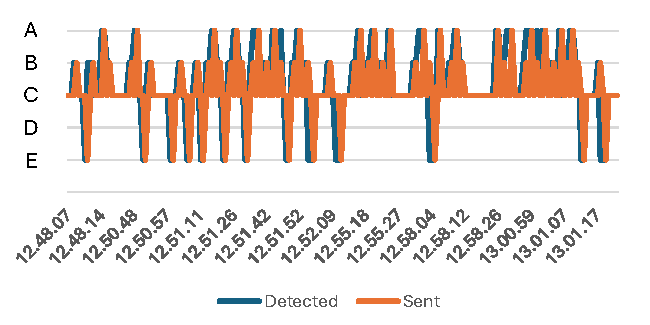
\includegraphics[width=1\textwidth]{gambar/tex/sents.pdf}
    \caption{Detection and Transmission Plots.}
    \label{fig:detection_transmission_plots}
\end{figure}

Visualisasi pada gambar \ref{fig:detection_transmission_plots} berperan penting dalam mendeteksi adanya anomali atau kesalahan yang mungkin terjadi selama proses pengujian. Data yang dipilih untuk divisualisasikan merupakan salah satu hasil terbaik dari serangkaian percobaan terpisah yang telah dilakukan. Hal ini menunjukkan bahwa data tersebut merepresentasikan kondisi sistem yang optimal dan relevan untuk dianalisis lebih lanjut.

\begin{table}[H]
    \centering
    \caption{Summary of Data Transmission and Detection}
    \label{tab:summary_data_transmission_detection}
    \begin{tabular}{|c|c|}
        \hline 
        \cellcolor[HTML]{000000} & \cellcolor[HTML]{C0C0C0} \textbf{Percentage}   \\ \hline
        \cellcolor[HTML]{C0C0C0} \textbf{Transmitted as \texttt{C}} & 55.4  \\ \hline
        \cellcolor[HTML]{C0C0C0} \textbf{Same Register}  & 38.3 \\ \hline
        \cellcolor[HTML]{C0C0C0} \textbf{Different Register}  & 6.3 \\ \hline
    \end{tabular}
\end{table}

Tabel \ref{tab:summary_data_transmission_detection} merangkum data transmisi dan deteksi. Persentase data yang dikirim sebagai \texttt{C} adalah 55.4\%, yang menunjukkan bahwa sistem sering mengirim instruksi untuk berhenti. Persentase data di mana deteksi dan data yang dikirim sama adalah 38.3\%, yang menunjukkan bahwa sistem berjalan sesuai dengan deteksi yang dilakukan. Persentase data di mana deteksi dan data yang dikirim berbeda adalah 6.3\%, yang menunjukkan adanya galat atau kesalahan dalam sistem.

\newpage
\subsection{Percobaan Bergerak Maju}
\label{subsec:percobaanbergerakmaju}

Bagian ini membahas kemampuan sistem dalam mengikuti objek yang bergerak maju dengan kecepatan konstan. Tantangan yang dihadapi adalah bagaimana sistem mempertahankan objek dalam frame sambil melakukan penyesuaian kecepatan yang diperlukan. Solusinya meliputi pemanfaatan fusi data dari YOLOv11 dan MediaPipe Pose, serta penerapan algoritma kontrol yang mampu melakukan koreksi arah tepat waktu, sehingga sistem dapat mengikuti objek yang bergerak maju dengan stabil dan akurat.

\begin{table}[H]
    \centering
    \caption{Data Performa Bergerak Maju}
    \label{tab:performa_bergerak_maju}
    \begin{tabular}{|c|c|c|c|c|c|c|c|}
    \hline
    Waktu & Reg (s) & YOLO (m) & MP (m) & x (px) & Deteksi & Terkirim & Keterangan \\ \hline
    12.48.09 & 0.2991 & 5.6875 & 46.1146 & 484 & b'B\textbackslash n' & b'E\textbackslash n' & Forward \\ \hline
    12.48.10 & 0.2516 & 2.2093 & 5.6063 & 595 & b'B\textbackslash n' & b'C\textbackslash n' & Forward \\ \hline
    12.48.17 & 2.6621 & 1.7109 & 3.1479 & 447 & b'B\textbackslash n' & b'C\textbackslash n' & Forward \\ \hline
    12.50.45 & 0.5046 & 2.5900 & 5.4523 & 391 & b'B\textbackslash n' & b'C\textbackslash n' & Forward \\ \hline
    12.50.46 & 0.3870 & 2.5980 & 4.9960 & 414 & b'B\textbackslash n' & b'B\textbackslash n' & Forward \\ \hline
    12.50.54 & 2.5388 & 1.4768 & 3.1208 & 501 & b'B\textbackslash n' & b'C\textbackslash n' & Forward \\ \hline
    12.51.00 & 0.3556 & 1.7144 & 1.5984 & 492 & b'B\textbackslash n' & b'C\textbackslash n' & Forward \\ \hline
    12.51.00 & 0.3290 & 1.4978 & 1.4964 & 466 & b'B\textbackslash n' & b'B\textbackslash n' & Forward \\ \hline
    12.51.08 & 0.3129 & 1.6801 & 1.7017 & 525 & b'B\textbackslash n' & b'C\textbackslash n' & Forward \\ \hline
    12.51.09 & 0.3226 & 1.6408 & 1.7256 & 463 & b'B\textbackslash n' & b'B\textbackslash n' & Forward \\ \hline
    12.51.17 & 5.5467 & 2.2628 & 2.6525 & 563 & b'B\textbackslash n' & b'C\textbackslash n' & Forward \\ \hline
    12.51.17 & 0.3035 & 1.9853 & 2.1709 & 408 & b'B\textbackslash n' & b'B\textbackslash n' & Forward \\ \hline
    12.51.21 & 2.9916 & 2.0186 & 3.1728 & 440 & b'B\textbackslash n' & b'C\textbackslash n' & Forward \\ \hline
    12.51.21 & 0.3446 & 2.4830 & 3.1701 & 601 & b'B\textbackslash n' & b'B\textbackslash n' & Forward \\ \hline
    12.51.26 & 3.8579 & 2.5354 & 2.0134 & 553 & b'B\textbackslash n' & b'C\textbackslash n' & Forward \\ \hline
    12.51.30 & 3.3993 & 2.4258 & 2.4468 & 551 & b'B\textbackslash n' & b'C\textbackslash n' & Forward \\ \hline
    12.51.36 & 4.6957 & 1.7144 & 1.8941 & 478 & b'B\textbackslash n' & b'C\textbackslash n' & Forward \\ \hline
    12.51.42 & 0.2820 & 1.4820 & 2.5157 & 424 & b'B\textbackslash n' & b'C\textbackslash n' & Forward \\ \hline
    12.51.42 & 0.2867 & 1.5473 & 1.6206 & 481 & b'B\textbackslash n' & b'B\textbackslash n' & Forward \\ \hline
    12.51.44 & 0.2619 & 1.6003 & 1.9633 & 426 & b'B\textbackslash n' & b'A\textbackslash n' & Forward \\ \hline
    12.51.45 & 0.2692 & 1.5704 & 1.6022 & 449 & b'B\textbackslash n' & b'C\textbackslash n' & Forward \\ \hline
    12.51.51 & 2.5508 & 2.2628 & 1.8379 & 569 & b'B\textbackslash n' & b'C\textbackslash n' & Forward \\ \hline
    12.51.52 & 0.6972 & 1.9174 & 2.2452 & 394 & b'B\textbackslash n' & b'B\textbackslash n' & Forward \\ \hline
    12.51.55 & 0.3125 & 1.9262 & 2.1721 & 564 & b'B\textbackslash n' & b'C\textbackslash n' & Forward \\ \hline
    12.52.05 & 0.2830 & 1.9395 & 2.9075 & 502 & b'B\textbackslash n' & b'C\textbackslash n' & Forward \\ \hline
    12.55.13 & 0.3498 & 2.0186 & 1.9290 & 520 & b'B\textbackslash n' & b'C\textbackslash n' & Forward \\ \hline
    12.55.14 & 0.3321 & 1.8664 & 2.8010 & 511 & b'B\textbackslash n' & b'B\textbackslash n' & Forward \\ \hline
    12.55.18 & 0.2536 & 1.2489 & 1.0783 & 483 & b'B\textbackslash n' & b'C\textbackslash n' & Forward \\ \hline
    12.55.18 & 0.3409 & 1.2734 & 1.0403 & 522 & b'B\textbackslash n' & b'B\textbackslash n' & Forward \\ \hline
    12.55.22 & 0.3309 & 1.5194 & 3.5842 & 504 & b'B\textbackslash n' & b'C\textbackslash n' & Forward \\ \hline
    \end{tabular}
\end{table}

Tabel \ref{tab:performa_bergerak_maju} menunjukkan data performa sistem saat bergerak maju. Data ini mencakup waktu deteksi, jarak deteksi dari YOLOv11 dan MediaPipe Pose, posisi objek dalam frame, hasil deteksi, instruksi yang dikirimkan, dan keterangan mengenai arah gerak. Data ini memberikan gambaran kinerja sistem dalam mengikuti objek yang bergerak maju, termasuk kecepatan respons, akurasi deteksi, dan ketepatan instruksi yang dikirimkan.

\begin{figure}[H]
    \centering
    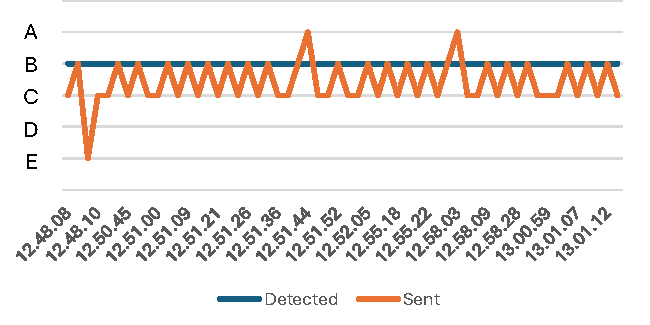
\includegraphics[width=1\textwidth]{gambar/tex/forward.pdf}
    \caption{Straight Movement Plots}
    \label{fig:straight_movement_plots}
\end{figure}

Visualisasi pada gambar \ref{fig:straight_movement_plots} berperan penting dalam mendeteksi adanya anomali atau kesalahan yang mungkin terjadi selama proses pengujian. Data yang dipilih untuk divisualisasikan merupakan salah satu hasil terbaik dari serangkaian percobaan terpisah yang telah dilakukan. Hal ini menunjukkan bahwa data tersebut merepresentasikan kondisi sistem yang optimal dan relevan untuk dianalisis lebih lanjut.

\begin{table}[H]
    \centering
    \caption{Summary of Data During Straight Movement}
    \label{tab:straight_movement_data_transmission_detection}
    \begin{tabular}{|c|c|}
        \hline 
        \cellcolor[HTML]{000000} & \cellcolor[HTML]{C0C0C0} \textbf{Percentage}   \\ \hline
        \cellcolor[HTML]{C0C0C0} \textbf{Transmitted as \texttt{C}} & 15.4  \\ \hline
        \cellcolor[HTML]{C0C0C0} \textbf{Same Register}  & 11.0  \\ \hline
        \cellcolor[HTML]{C0C0C0} \textbf{Different Register}   & 1.5  \\ \hline
    \end{tabular}
\end{table}

Tabel \ref{tab:straight_movement_data_transmission_detection} merangkum data transmisi dan deteksi selama gerakan maju. Persentase data yang dikirim sebagai \texttt{C} adalah 15.4\%, yang menunjukkan bahwa sistem sering mengirim instruksi untuk berhenti. Persentase data di mana deteksi dan data yang dikirim sama adalah 11.0\%, yang menunjukkan bahwa sistem berjalan sesuai dengan deteksi yang dilakukan. Persentase data di mana deteksi dan data yang dikirim berbeda adalah 1.5\%, yang menunjukkan adanya galat atau kesalahan dalam sistem.

\newpage
\subsection{Percobaan Belok Kiri}
\label{subsec:percobaanbelokkiri}

Bagian ini membahas kemampuan sistem dalam mengikuti objek saat berbelok ke kiri. Pada kondisi ini, tantangan yang muncul meliputi perubahan posisi relatif yang terjadi lebih cepat, potensi kehilangan objek dari frame, serta perlunya adaptasi kecepatan motor penggerak. Solusi yang diterapkan adalah penyesuaian parameter kontrol, algoritma pendeteksi pose yang lebih adaptif, serta strategi gerak yang mempertimbangkan arah belok objek sehingga sistem dapat mempertahankan jarak optimal dan ketepatan manuver ke kiri.

\begin{table}[H]
    \centering
    \caption{Data Performa Belok (Kiri)}
    \label{tab:performa_belok_kiri}
    \begin{tabular}{|c|c|c|c|c|c|c|c|c|}
    \hline
    Waktu & Reg (s) & YOLO (m) & MP (m) & x (px) & Deteksi & Terkirim & Keterangan \\ \hline
    12:48:14 & 2.7739 & 1.4513 & 1.1409 & 128 & b'A\textbackslash n' & b'C\textbackslash n' & Turn Left \\ \hline
    12:50:48 & 2.7333 & 1.1421 & 1.0733 & 164 & b'A\textbackslash n' & b'C\textbackslash n' & Turn Left \\ \hline
    12:51:18 & 0.3176 & 1.6668 & 1.1184 & 189 & b'A\textbackslash n' & b'C\textbackslash n' & Turn Left \\ \hline
    12:51:18 & 0.3818 & 1.5277 & 1.1295 & 202 & b'A\textbackslash n' & b'A\textbackslash n' & Turn Left \\ \hline
    12:51:26 & 0.4472 & 1.9174 & 1.4873 & 212 & b'A\textbackslash n' & b'C\textbackslash n' & Turn Left \\ \hline
    12:51:27 & 0.2536 & 1.6668 & 1.2112 & 142 & b'A\textbackslash n' & b'A\textbackslash n' & Turn Left \\ \hline
    12:51:37 & 1.7377 & 1.5194 & 1.4537 & 182 & b'A\textbackslash n' & b'B\textbackslash n' & Turn Left \\ \hline
    12:51:44 & 0.3591 & 2.1528 & 1.7878 & 245 & b'A\textbackslash n' & b'C\textbackslash n' & Turn Left \\ \hline
    12:51:45 & 0.3616 & 1.8259 & 1.5129 & 249 & b'A\textbackslash n' & b'B\textbackslash n' & Turn Left \\ \hline
    12:51:52 & 0.3755 & 1.5912 & 1.3909 & 185 & b'A\textbackslash n' & b'C\textbackslash n' & Turn Left \\ \hline
    12:51:52 & 0.3613 & 1.4716 & 1.2101 & 174 & b'A\textbackslash n' & b'A\textbackslash n' & Turn Left \\ \hline
    12:55:15 & 1.6785 & 1.1238 & 1.0672 & 170 & b'A\textbackslash n' & b'C\textbackslash n' & Turn Left \\ \hline
    12:55:18 & 0.3224 & 1.2129 & 1.4666 & 168 & b'A\textbackslash n' & b'C\textbackslash n' & Turn Left \\ \hline
    12:55:19 & 0.3399 & 1.1515 & 1.3422 & 165 & b'A\textbackslash n' & b'A\textbackslash n' & Turn Left \\ \hline
    12:55:25 & 0.4715 & 1.1164 & 1.4924 & 170 & b'A\textbackslash n' & b'C\textbackslash n' & Turn Left \\ \hline
    12:58:05 & 0.4054 & 1.3446 & 1.3906 & 174 & b'A\textbackslash n' & b'A\textbackslash n' & Turn Left \\ \hline
    12:58:10 & 1.2931 & 1.4123 & 1.6479 & 320 & b'A\textbackslash n' & b'C\textbackslash n' & Turn Left \\ \hline
    12:58:25 & 4.1776 & 1.1047 & 1.2300 & 197 & b'A\textbackslash n' & b'C\textbackslash n' & Turn Left \\ \hline
    12:58:26 & 0.6310 & 1.1284 & 1.2368 & 195 & b'A\textbackslash n' & b'A\textbackslash n' & Turn Left \\ \hline
    13:00:55 & 1.9408 & 1.0975 & 1.0855 & 185 & b'A\textbackslash n' & b'C\textbackslash n' & Turn Left \\ \hline
    13:00:55 & 0.4380 & 1.0975 & 1.1142 & 177 & b'A\textbackslash n' & b'C\textbackslash n' & Turn Left \\ \hline
    13:00:56 & 0.3263 & 1.0960 & 1.1078 & 167 & b'A\textbackslash n' & b'A\textbackslash n' & Turn Left \\ \hline
    13:00:58 & 0.2737 & 1.6903 & 1.0003 & 215 & b'A\textbackslash n' & b'B\textbackslash n' & Turn Left \\ \hline
    13:00:59 & 0.2535 & 1.6869 & 1.4439 & 228 & b'A\textbackslash n' & b'C\textbackslash n' & Turn Left \\ \hline
    13:00:59 & 0.3323 & 1.7536 & 1.3650 & 225 & b'A\textbackslash n' & b'A\textbackslash n' & Turn Left \\ \hline
    13:01:00 & 0.3113 & 1.2734 & 1.1814 & 173 & b'A\textbackslash n' & b'B\textbackslash n' & Turn Left \\ \hline
    13:01:01 & 0.4180 & 1.6188 & 1.0805 & 170 & b'A\textbackslash n' & b'C\textbackslash n' & Turn Left \\ \hline
    13:01:02 & 0.2600 & 1.5882 & 1.5507 & 222 & b'A\textbackslash n' & b'A\textbackslash n' & Turn Left \\ \hline
    13:01:08 & 0.4923 & 1.6188 & 1.3519 & 211 & b'A\textbackslash n' & b'C\textbackslash n' & Turn Left \\ \hline
    13:01:09 & 0.3287 & 1.7039 & 1.7476 & 202 & b'A\textbackslash n' & b'A\textbackslash n' & Turn Left \\ \hline
\end{tabular}
\end{table}

Table \ref{tab:performa_belok_kiri} menunjukkan data performa sistem saat berbelok ke kiri. Data ini mencakup waktu deteksi, jarak deteksi dari YOLOv11 dan MediaPipe Pose, posisi objek dalam frame, hasil deteksi, instruksi yang dikirimkan, dan keterangan mengenai arah belok. Data ini memberikan gambaran kinerja sistem dalam mengikuti objek yang berbelok ke kiri, termasuk kecepatan respons, akurasi deteksi, dan ketepatan instruksi yang dikirimkan.

\begin{figure}[H]
    \centering
    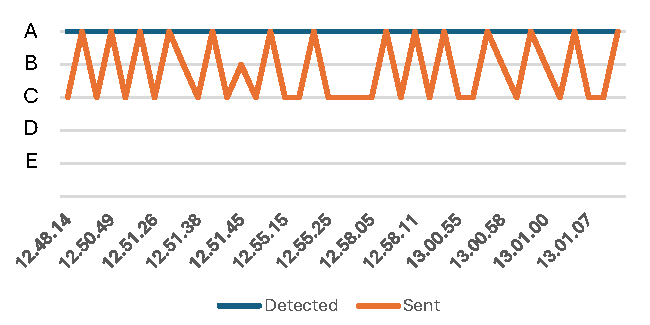
\includegraphics[width=1\textwidth]{gambar/tex/left.pdf}
    \caption{Left Turn Plots}
    \label{fig:left_turn_plots}
\end{figure}

Visualisasi pada gambar \ref{fig:left_turn_plots} berperan penting dalam mendeteksi adanya anomali atau kesalahan yang mungkin terjadi selama proses pengujian. Data yang dipilih untuk divisualisasikan merupakan salah satu hasil terbaik dari serangkaian percobaan terpisah yang telah dilakukan. Hal ini menunjukkan bahwa data tersebut merepresentasikan kondisi sistem yang optimal dan relevan untuk dianalisis lebih lanjut.

\begin{table}[H]
    \centering
    \caption{Summary of Data During Left Turn}
    \label{tab:left_turn_data_transmission_detection}
    \begin{tabular}{|c|c|}
        \hline 
        \cellcolor[HTML]{000000} & \cellcolor[HTML]{C0C0C0} \textbf{Percentage}  \\ \hline
        \cellcolor[HTML]{C0C0C0} \textbf{Transmitted as \texttt{C}} & 10.5 \\ \hline
        \cellcolor[HTML]{C0C0C0} \textbf{Same Register}  & 6.7 \\ \hline
        \cellcolor[HTML]{C0C0C0} \textbf{Different Register}   & 2.0 \\ \hline
    \end{tabular}
\end{table}

Tabel \ref{tab:left_turn_data_transmission_detection} merangkum data transmisi dan deteksi selama belok kiri. Persentase data yang dikirim sebagai \texttt{C} adalah 10.5\%, yang menunjukkan bahwa sistem sering mengirim instruksi untuk berhenti. Persentase data di mana deteksi dan data yang dikirim sama adalah 6.7\%, yang menunjukkan bahwa sistem berjalan sesuai dengan deteksi yang dilakukan. Persentase data di mana deteksi dan data yang dikirim berbeda adalah 2.0\%, yang menunjukkan adanya galat atau kesalahan dalam sistem.

\newpage
\subsection{Percobaan Belok Kanan}
\label{subsec:percobaanbelokkanan}

Bagian ini membahas kemampuan sistem dalam mengikuti objek saat berbelok ke kanan, yang pada dasarnya serupa dengan kondisi belok kanan. Tantangan yang dihadapi adalah bagaimana sistem mempertahankan objek dalam frame sambil melakukan penyesuaian sudut belok yang diperlukan. Solusinya meliputi pemanfaatan fusi data dari YOLOv11 dan MediaPipe Pose, serta penerapan algoritma kontrol yang mampu melakukan koreksi arah tepat waktu, sehingga sistem dapat mengikuti objek yang berbelok ke kanan dengan stabil dan akurat.

\begin{table}[H]
    \centering
    \caption{Data Performa Belok (Kanan)}
    \label{tab:performa_belok_kanan}
    \begin{tabular}{|c|c|c|c|c|c|c|c|c|}
    \hline
    Waktu & Reg (s) & YOLO (m) & MP (m) & x (px) & Deteksi & Terkirim & Keterangan \\ \hline
    12:48:09 & 0.2960 & 2.4469 & 1.6214 & 765 & b'E\textbackslash n' & b'C\textbackslash n' & Turn Right \\ \hline
    12:50:51 & 0.4610 & 1.4219 & 1.0142 & 830 & b'E\textbackslash n' & b'C\textbackslash n' & Turn Right \\ \hline
    12:50:56 & 0.6617 & 2.0234 & 1.6721 & 801 & b'E\textbackslash n' & b'C\textbackslash n' & Turn Right \\ \hline
    12:50:07 & 0.3573 & 1.4291 & 1.4911 & 795 & b'E\textbackslash n' & b'B\textbackslash n' & Turn Right \\ \hline
    12:50:07 & 0.3236 & 1.4588 & 1.7653 & 820 & b'E\textbackslash n' & b'C\textbackslash n' & Turn Right \\ \hline
    12:50:57 & 0.2675 & 2.0939 & 1.4524 & 825 & b'E\textbackslash n' & b'E\textbackslash n' & Turn Right \\ \hline
    12:51:07 & 3.9922 & 1.7796 & 1.3830 & 896 & b'E\textbackslash n' & b'C\textbackslash n' & Turn Right \\ \hline
    12:51:07 & 0.3518 & 2.0345 & 1.5442 & 883 & b'E\textbackslash n' & b'E\textbackslash n' & Turn Right \\ \hline
    12:51:11 & 2.3641 & 1.5332 & 1.5242 & 850 & b'E\textbackslash n' & b'C\textbackslash n' & Turn Right \\ \hline
    12:51:11 & 0.2897 & 2.0453 & 1.7421 & 792 & b'E\textbackslash n' & b'E\textbackslash n' & Turn Right \\ \hline
    12:51:22 & 0.2721 & 2.6141 & 1.7926 & 769 & b'E\textbackslash n' & b'C\textbackslash n' & Turn Right \\ \hline
    12:51:22 & 0.2947 & 2.7330 & 1.5570 & 867 & b'E\textbackslash n' & b'E\textbackslash n' & Turn Right \\ \hline
    12:51:31 & 0.2615 & 2.5602 & 1.3594 & 879 & b'E\textbackslash n' & b'C\textbackslash n' & Turn Right \\ \hline
    12:51:31 & 0.2711 & 2.2042 & 1.3829 & 827 & b'E\textbackslash n' & b'E\textbackslash n' & Turn Right \\ \hline
    12:51:41 & 2.8133 & 1.7721 & 1.4401 & 766 & b'E\textbackslash n' & b'C\textbackslash n' & Turn Right \\ \hline
    12:51:47 & 0.3573 & 1.4291 & 1.4911 & 795 & b'E\textbackslash n' & b'B\textbackslash n' & Turn Right \\ \hline
    12:51:48 & 0.3236 & 1.4588 & 1.7653 & 820 & b'E\textbackslash n' & b'C\textbackslash n' & Turn Right \\ \hline
    12:51:48 & 0.2701 & 1.9485 & 1.6638 & 792 & b'E\textbackslash n' & b'E\textbackslash n' & Turn Right \\ \hline
    12:51:56 & 0.2506 & 1.9262 & 1.7147 & 880 & b'E\textbackslash n' & b'C\textbackslash n' & Turn Right \\ \hline
    12:51:56 & 0.2716 & 1.9759 & 1.6276 & 871 & b'E\textbackslash n' & b'E\textbackslash n' & Turn Right \\ \hline
    12:55:09 & 1.9217 & 1.5004 & 1.8914 & 861 & b'E\textbackslash n' & b'C\textbackslash n' & Turn Right \\ \hline
    12:55:10 & 0.3128 & 2.1414 & 1.8698 & 858 & b'E\textbackslash n' & b'C\textbackslash n' & Turn Right \\ \hline
    12:55:10 & 0.3967 & 2.7356 & 2.0821 & 856 & b'E\textbackslash n' & b'E\textbackslash n' & Turn Right \\ \hline
    12:58:04 & 0.3573 & 1.4291 & 1.4911 & 795 & b'E\textbackslash n' & b'B\textbackslash n' & Turn Right \\ \hline
    12:58:04 & 0.3236 & 1.4588 & 1.7653 & 820 & b'E\textbackslash n' & b'C\textbackslash n' & Turn Right \\ \hline
    12:58:05 & 0.3560 & 1.6768 & 1.8145 & 795 & b'E\textbackslash n' & b'E\textbackslash n' & Turn Right \\ \hline
    13:01:13 & 1.1224 & 1.8459 & 1.5848 & 850 & b'E\textbackslash n' & b'C\textbackslash n' & Turn Right \\ \hline
    13:01:13 & 0.2936 & 1.5942 & 1.0293 & 832 & b'E\textbackslash n' & b'E\textbackslash n' & Turn Right \\ \hline
    13:01:17 & 0.3835 & 1.1238 & 1.0723 & 862 & b'E\textbackslash n' & b'B\textbackslash n' & Turn Right \\ \hline
    13:01:18 & 0.3058 & 1.1253 & 1.0494 & 845 & b'E\textbackslash n' & b'C\textbackslash n' & Turn Right \\ \hline
\end{tabular}
\end{table}

Tabel \ref{tab:performa_belok_kanan} menunjukkan data performa sistem saat berbelok ke kanan. Data ini mencakup waktu deteksi, jarak deteksi dari YOLOv11 dan MediaPipe Pose, posisi objek dalam frame, hasil deteksi, instruksi yang dikirimkan, dan keterangan mengenai arah belok. Data ini memberikan gambaran kinerja sistem dalam mengikuti objek yang berbelok ke kanan, termasuk kecepatan respons, akurasi deteksi, dan ketepatan instruksi yang dikirimkan.

\begin{figure}[H]
    \centering
    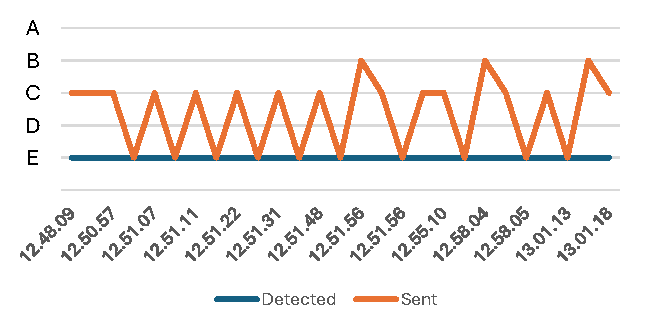
\includegraphics[width=1\textwidth]{gambar/tex/right.pdf}
    \caption{Right Turn Plots}
    \label{fig:right_turn_plots}
\end{figure}

Visualisasi pada gambar \ref{fig:right_turn_plots} berperan penting dalam mendeteksi adanya anomali atau kesalahan yang mungkin terjadi selama proses pengujian. Data yang dipilih untuk divisualisasikan merupakan salah satu hasil terbaik dari serangkaian percobaan terpisah yang telah dilakukan. Hal ini menunjukkan bahwa data tersebut merepresentasikan kondisi sistem yang optimal dan relevan untuk dianalisis lebih lanjut.

\begin{table}[H]
    \centering
    \caption{Summary of Data During Right Turn}
    \label{tab:right_turn_data_transmission_detection}
    \begin{tabular}{|c|c|}
        \hline 
        \cellcolor[HTML]{000000} & \cellcolor[HTML]{C0C0C0} \textbf{Percentage}   \\ \hline
        \cellcolor[HTML]{C0C0C0} \textbf{Transmitted as \texttt{C}} & 6.7  \\ \hline
        \cellcolor[HTML]{C0C0C0} \textbf{Same Register}  & 5.0  \\ \hline
        \cellcolor[HTML]{C0C0C0} \textbf{Different Register}   & 1.5  \\ \hline
    \end{tabular}
\end{table}

Tabel \ref{tab:right_turn_data_transmission_detection} merangkum data transmisi dan deteksi selama belok kanan. Persentase data yang dikirim sebagai \texttt{C} adalah 6.7\%, yang menunjukkan bahwa sistem sering mengirim instruksi untuk berhenti. Persentase data di mana deteksi dan data yang dikirim sama adalah 5.0\%, yang menunjukkan bahwa sistem berjalan sesuai dengan deteksi yang dilakukan. Persentase data di mana deteksi dan data yang dikirim berbeda adalah 1.5\%, yang menunjukkan adanya galat atau kesalahan dalam sistem.

\newpage
\subsection{Percobaan Luar Frame}
\label{subsec:percobaanluarframe}

Bagian ini membahas kemampuan sistem dalam menghadapi kondisi ketika objek keluar dari bidang pandang kamera (luar frame). Tantangan yang muncul adalah hilangnya data visual tentang posisi dan gerakan objek, sehingga sistem harus mampu memprediksi posisi berikutnya atau melakukan penyesuaian strategi pencarian. Solusi yang digunakan mencakup pengintegrasian algoritma prediksi lintasan serta inisialisasi ulang posisi, yang membantu sistem untuk kembali melacak objek setelah objek kembali ke dalam frame.

\begin{table}[H]
    \centering
    \caption{Data Status Frame (Luar Frame)}
    \label{tab:status_luar_frame}
    \begin{tabular}{|c|c|c|c|c|c|c|c|c|}
    \hline
    Waktu & Reg (s) & YOLO (m) & MP (m) & x (px) & Deteksi & Terkirim & Keterangan \\ \hline
    12:48:08 & 0.2758 & 0.0 & 0.0 & 0 & b'B\textbackslash n' & b'B\textbackslash n' & Forward \\ \hline
    12:48:08 & 0.3151 & 0.0 & 0.0 & 0 & b'B\textbackslash n' & b'B\textbackslash n' & Forward \\ \hline
    12:48:15 & 0.2931 & 0.0 & 0.0 & 0 & b'A\textbackslash n' & b'A\textbackslash n' & Turn Left \\ \hline
    12:48:18 & 0.3001 & 0.0 & 0.0 & 0 & b'B\textbackslash n' & b'B\textbackslash n' & Forward \\ \hline
    12:50:43 & 0.7366 & 0.0 & 0.0 & 0 & b'C\textbackslash n' & b'C\textbackslash n' & Stop \\ \hline
    12:50:43 & 0.3732 & 0.0 & 0.0 & 0 & b'C\textbackslash n' & b'C\textbackslash n' & Stop \\ \hline
    12:50:43 & 0.2571 & 0.0 & 0.0 & 0 & b'C\textbackslash n' & b'C\textbackslash n' & Stop \\ \hline
    12:50:44 & 0.2395 & 0.0 & 0.0 & 0 & b'E\textbackslash n' & b'E\textbackslash n' & Turn Right \\ \hline
    12:50:44 & 0.3522 & 0.0 & 0.0 & 0 & b'C\textbackslash n' & b'C\textbackslash n' & Stop \\ \hline
    12:50:44 & 0.3647 & 0.0 & 0.0 & 0 & b'C\textbackslash n' & b'C\textbackslash n' & Stop \\ \hline
    12:50:45 & 0.3504 & 0.0 & 0.0 & 0 & b'C\textbackslash n' & b'C\textbackslash n' & Stop \\ \hline
    12:50:49 & 0.3535 & 0.0 & 0.0 & 0 & b'A\textbackslash n' & b'A\textbackslash n' & Turn Left \\ \hline
    12:51:07 & 0.3518 & 0.0 & 0.0 & 0 & b'E\textbackslash n' & b'E\textbackslash n' & Turn Right \\ \hline
    12:51:11 & 0.2897 & 0.0 & 0.0 & 0 & b'E\textbackslash n' & b'E\textbackslash n' & Turn Right \\ \hline
    12:51:26 & 0.3185 & 0.0 & 0.0 & 0 & b'B\textbackslash n' & b'B\textbackslash n' & Forward \\ \hline
    12:51:30 & 0.2687 & 0.0 & 0.0 & 0 & b'B\textbackslash n' & b'B\textbackslash n' & Forward \\ \hline
    12:51:31 & 0.2615 & 0.0 & 0.0 & 0 & b'E\textbackslash n' & b'E\textbackslash n' & Turn Right \\ \hline
    12:51:31 & 0.2711 & 0.0 & 0.0 & 0 & b'E\textbackslash n' & b'E\textbackslash n' & Turn Right \\ \hline
    12:51:38 & 0.2502 & 0.0 & 0.0 & 0 & b'A\textbackslash n' & b'A\textbackslash n' & Turn Left \\ \hline
    12:51:38 & 0.2617 & 0.0 & 0.0 & 0 & b'A\textbackslash n' & b'A\textbackslash n' & Turn Left \\ \hline
    12:52:05 & 0.6562 & 0.0 & 0.0 & 0 & b'B\textbackslash n' & b'B\textbackslash n' & Forward \\ \hline
    12:58:09 & 0.3319 & 0.0 & 0.0 & 0 & b'B\textbackslash n' & b'B\textbackslash n' & Forward \\ \hline
    12:58:11 & 0.2506 & 0.0 & 0.0 & 0 & b'A\textbackslash n' & b'A\textbackslash n' & Turn Left \\ \hline
    13:00:57 & 0.3574 & 0.0 & 0.0 & 0 & b'C\textbackslash n' & b'C\textbackslash n' & Stop \\ \hline
    13:01:07 & 0.2856 & 0.0 & 0.0 & 0 & b'A\textbackslash n' & b'A\textbackslash n' & Turn Left \\ \hline
    13:01:12 & 0.2639 & 0.0 & 0.0 & 0 & b'B\textbackslash n' & b'B\textbackslash n' & Forward \\ \hline
    13:01:16 & 1.3214 & 0.0 & 0.0 & 0 & b'C\textbackslash n' & b'C\textbackslash n' & Stop \\ \hline
    13:01:16 & 0.3159 & 0.0 & 0.0 & 0 & b'C\textbackslash n' & b'C\textbackslash n' & Stop \\ \hline
    13:01:17 & 0.3360 & 0.0 & 0.0 & 0 & b'C\textbackslash n' & b'C\textbackslash n' & Stop \\ \hline
    13:01:19 & 0.2638 & 0.0 & 0.0 & 0 & b'C\textbackslash n' & b'C\textbackslash n' & Stop \\ \hline
    \end{tabular}
\end{table}
Tabel \ref{tab:status_luar_frame} menunjukkan data status sistem saat objek berada di luar frame. Data ini memperlihatkan saat nilai dari deteksi objek keduanya adalah 0 dan keterangan mengenai status objek. Data ini memberikan gambaran kinerja sistem dalam menghadapi kondisi ketika objek keluar dari bidang pandang kamera, termasuk kecepatan respons, akurasi deteksi, dan ketepatan instruksi yang dikirimkan.

Beberapa data telah difilter untuk menampilkan data yang menunjukkan sistem bekerja dengan sempurna ketika tidak ada objek yang terdeteksi dan mengirimkan kode instruksi sebelumnya tanpa penundaan yang lama ke mesin. Namun, ada masalah serius di mana sistem terus-menerus mengirimkan kode instruksi maju tanpa jaminan bahwa objek akan terdeteksi untuk mengubah kode instruksi ke mesin. Hal ini dapat menyebabkan potensi risiko keselamatan dan ketidakefisienan dalam operasi sistem.

\section{Performa Keberhasilan Mengikuti}
\label{sec:performamengikuti}

Bagian ini menguji apakah sistem dapat mengikuti objek pada lajur khusus, seperti jalur sempit atau berbelok yang membutuhkan manuver khusus.

\section{Pembahasan Hasil}
\label{sec:pembahasanhasil}

Bagian ini membahas hasil-hasil pengujian secara keseluruhan dan memberikan insight mengenai performa sistem.

\subsection{Performa Deteksi Objek}
\label{sec:performadeteksiobjek}

Bagian ini menjelaskan kekuatan dan kelemahan deteksi objek yang ditemukan selama pengujian.

\subsection{Kecepatan Pemrosesan (FPS)}
\label{sec:kecepatanpemrosesan}

Menganalisis kecepatan pemrosesan secara keseluruhan dan pengaruhnya terhadap performa sistem real-time.

\subsection{Response Time}
\label{sec:responsetime}

Membahas hasil pengujian response time dan faktor-faktor yang mempengaruhi waktu respons.

\subsection{Keberhasilan Tracking}
\label{sec:performatracking}

Membahas tingkat keberhasilan sistem dalam melacak objek dan kondisi yang mempengaruhi performa.

\subsection{Kesesuaian Tingkat Pencahayaan}
\label{sec:kesesuaianpencahayaan}

Membahas tingkat keberhasilan sistem dalam melacak objek pada kondisi pencahayaan yang berbeda.

\subsection{Kesesuaian Jarak Deteksi}
\label{sec:kesesuaianjarak}

Diskusi tentang performa sistem dalam mendeteksi objek pada berbagai jarak yang telah diuji.

\subsection{Performa Pergerakan Mengikuti Objek}
\label{sec:akurasiikutiobjek}

Evaluasi akurasi dalam mengikuti objek target, termasuk kondisi yang dapat menyebabkan kegagalan.

\subsection{Performa Keberhasilan Mengikuti}
\label{sec:keberhasilanmengikuti}

Menguraikan keberhasilan sistem dalam mengikuti objek saat menghadapi belokan dan lajur khusus.
\cleardoublepage

% Bab 5 penutup
\chapter{PENUTUP}
\label{chap:penutup}

% Ubah bagian-bagian berikut dengan isi dari penutup

\section{Kesimpulan}
\label{sec:kesimpulan}

Berdasarkan hasil pengujian yang telah dilakukan, dapat diambil kesimpulan sebagai berikut:

\begin{enumerate}[nolistsep]
  \item Model menunjukkan performa deteksi yang tinggi dengan skor mAP mencapai 81.85\% pada threshold 0.5.
  \item Sistem mampu memproses frame secara real-time dengan rata-rata FPS sekitar 40, menunjukkan kecepatan pemrosesan yang memadai untuk aplikasi lapangan.
  \item Pengujian regulator time menunjukkan bahwa 66.17\% respons berada dalam waktu yang relatif singkat, namun 34\% lainnya melebihi 0.5 detik.
  \item Sistem berhasil mengunci target (Locked Detection) sebanyak 4 kali dari 15 percobaan, menghasilkan tingkat keberhasilan sebesar 26.67\%.
  \item Sistem menunjukkan kinerja terbaik pada kondisi pencahayaan optimal, namun kinerja menurun pada kondisi pencahayaan rendah.
  \item Sistem mampu mendeteksi objek dengan jarak kurang dari 1 meter secara konsisten dan mengirimkan instruksi "Stop" untuk mencegah tabrakan.
  \item Sistem memiliki performa yang sangat baik dalam mendeteksi dan mengikuti objek di berbagai skenario, baik saat dalam frame, bergerak maju, maupun berbelok.
  \item Sistem mampu mengikuti objek dengan baik di seluruh kondisi jalur yang diuji, dengan tingkat keberhasilan mencapai 100\%.

\end{enumerate}

\section{Saran}
\label{chap:saran}

Untuk pengembangan lebih lanjut pada penelitian selanjutnya, adapun saran yang bisa diberikan antara lain:

\begin{enumerate}[nolistsep]
  \item Meningkatkan fungsi \texttt{track()} untuk menjaga konsistensi identitas ID objek yang terdeteksi, guna meningkatkan akurasi pelacakan.
  \item Menggunakan pencahayaan tambahan yang tidak menyebabkan overexposure dapat dipertimbangkan untuk meningkatkan kinerja deteksi pada kondisi pencahayaan rendah.
  \item Memberikan optimisasi lebih lanjut pada sistem untuk mengurangi waktu respons yang melebihi 0.5 detik, guna meningkatkan stabilitas dan konsistensi kinerja.
  \item Menuliskan algoritma yang lebih adaptif untuk menangani kondisi luar frame, sehingga dapat mencegah pengiriman instruksi yang tidak relevan atau tidak aman.
  \item Implementasi sistem pada skenario nyata dengan berbagai kondisi operasional untuk menguji dan memastikan keandalan serta keamanan sistem secara menyeluruh.
\end{enumerate}

\cleardoublepage

\chapter*{DAFTAR PUSTAKA}
\addcontentsline{toc}{chapter}{DAFTAR PUSTAKA}
\renewcommand\refname{}
\vspace{2ex}
\renewcommand{\bibname}{}
\begingroup
\def\chapter*#1{}
\printbibliography
\endgroup
\cleardoublepage

% Bab 6 lampiran
\begin{center}
    \Large
    \textbf{LAMPIRAN}
\end{center}

\phantomsection
\addcontentsline{toc}{chapter}{LAMPIRAN}

\vspace{2ex}

\textbf{Kode Program}

\phantomsection
\addcontentsline{toc}{section}{Kode Program}

\lstinputlisting[
  language=Python,
  caption={Program Deteksi Fusi pada Unit Kontrol.},
  label={lst:deteksifusi}
]{program/pameran.py}

\lstinputlisting[
  language=C++,
  caption={Program Stream Frame dan Forward Kode Instruksi.},
  label={lst:ESP32CAM}
]{program/ESP32-Camera-AP.ino}

\lstinputlisting[
  language=C++,
  caption={Program Pengolahan Kode Instruksi Pada Motor.},
  label={lst:ESP32Motor}
]{program/ESP-NOW-Motor.ino}


\cleardoublepage

% Biografi penulis
\begin{center}
  \Large
  \textbf{BIOGRAFI PENULIS}
\end{center}

\addcontentsline{toc}{chapter}{BIOGRAFI PENULIS}

\vspace{2ex}

\begin{wrapfigure}{L}{0.3\textwidth}
  \centering
  \vspace{-3ex}
  % Ubah file gambar berikut dengan file foto dari mahasiswa
  \includegraphics[width=0.3\textwidth]{gambar/IMG_4170.jpg}
  \vspace{-4ex}
\end{wrapfigure}

% Ubah kalimat berikut dengan biografi dari mahasiswa
\name{}, lahir pada 24 Mei 2000 di kota Padangsidimpuan. Penulis merupakan anak ketiga dari 3 bersaudara.
Setelah lulus dari MA Negeri 2 Padangsidimpuan, Penulis kemudian melanjutkan pendidikan ke jenjang strata satu di Departemen Teknik Komputer ITS, Fakultas Teknologi Elektro dan Informatika Cerdas, Institut Teknologi Sepuluh Nopember mulai tahun 2018.

Penulis merupakan orang yang aktif berorganisasi, dan memiliki berbagai softskill serta hardskill. Hal ini dibuktikan dengan rekam jejak organisasi dan kepanitiaan dari penulis seperti Staff Hima Teknik komputer ITS, Bangkit Academy Mobile Development.

\cleardoublepage

\end{document}
